% Template for PLoS
%DIF LATEXDIFF DIFFERENCE FILE
%DIF DEL original.tex   Wed Oct  7 15:01:39 2020
%DIF ADD review_1.tex   Wed Oct  7 15:35:26 2020
% Version 3.5 March 2018
%
% % % % % % % % % % % % % % % % % % % % % %
%
% -- IMPORTANT NOTE
%
% This template contains comments intended 
% to minimize problems and delays during our production 
% process. Please follow the template instructions
% whenever possible.
%
% % % % % % % % % % % % % % % % % % % % % % % 
%
% Once your paper is accepted for publication, 
% PLEASE REMOVE ALL TRACKED CHANGES in this file 
% and leave only the final text of your manuscript. 
% PLOS recommends the use of latexdiff to track changes during review, as this will help to maintain a clean tex file.
% Visit https://www.ctan.org/pkg/latexdiff?lang=en for info or contact us at latex@plos.org.
%
%
% There are no restrictions on package use within the LaTeX files except that 
% no packages listed in the template may be deleted.
%
% Please do not include colors or graphics in the text.
%
% The manuscript LaTeX source should be contained within a single file (do not use \input, \externaldocument, or similar commands).
%
% % % % % % % % % % % % % % % % % % % % % % %
%
% -- FIGURES AND TABLES
%
% Please include tables/figure captions directly after the paragraph where they are first cited in the text.
%
% DO NOT INCLUDE GRAPHICS IN YOUR MANUSCRIPT
% - Figures should be uploaded separately from your manuscript file. 
% - Figures generated using LaTeX should be extracted and removed from the PDF before submission. 
% - Figures containing multiple panels/subfigures must be combined into one image file before submission.
% For figure citations, please use "Fig" instead of "Figure".
% See http://journals.plos.org/plosone/s/figures for PLOS figure guidelines.
%
% Tables should be cell-based and may not contain:
% - spacing/line breaks within cells to alter layout or alignment
% - do not nest tabular environments (no tabular environments within tabular environments)
% - no graphics or colored text (cell background color/shading OK)
% See http://journals.plos.org/plosone/s/tables for table guidelines.
%
% For tables that exceed the width of the text column, use the adjustwidth environment as illustrated in the example table in text below.
%
% % % % % % % % % % % % % % % % % % % % % % % %
%
% -- eqnarrayS, MATH SYMBOLS, SUBSCRIPTS, AND SUPERSCRIPTS
%
% IMPORTANT
% Below are a few tips to help format your eqnarrays and other special characters according to our specifications. For more tips to help reduce the possibility of formatting errors during conversion, please see our LaTeX guidelines at http://journals.plos.org/plosone/s/latex
%
% For inline eqnarrays, please be sure to include all portions of an eqnarray in the math environment.  For example, x$^2$ is incorrect; this should be formatted as $x^2$ (or $\mathrm{x}^2$ if the romanized font is desired).
%
% Do not include text that is not math in the math environment. For example, CO2 should be written as CO\textsubscript{2} instead of CO$_2$.
%
% Please add line breaks to long display eqnarrays when possible in order to fit size of the column. 
%
% For inline eqnarrays, please do not include punctuation (commas, etc) within the math environment unless this is part of the eqnarray.
%
% When adding superscript or subscripts outside of brackets/braces, please group using {}.  For example, change "[U(D,E,\gamma)]^2" to "{[U(D,E,\gamma)]}^2". 
%
% Do not use \cal for caligraphic font.  Instead, use \mathcal{}
%
% % % % % % % % % % % % % % % % % % % % % % % % 
%
% Please contact latex@plos.org with any questions.
%
% % % % % % % % % % % % % % % % % % % % % % % %

\documentclass[10pt,letterpaper]{article}
\usepackage[top=0.85in,left=2.75in,footskip=0.75in]{geometry}

% amsmath and amssymb packages, useful for mathematical formulas and symbols
\usepackage{amsmath,amssymb}

% Use adjustwidth environment to exceed column width (see example table in text)
\usepackage{changepage}

% Use Unicode characters when possible
\usepackage[utf8x]{inputenc}

% textcomp package and marvosym package for additional characters
\usepackage{textcomp,marvosym}

% cite package, to clean up citations in the main text. Do not remove.
\usepackage{cite}

% Use nameref to cite supporting information files (see Supporting Information section for more info)
\usepackage{nameref,hyperref}

% line numbers
\usepackage[right]{lineno}

% ligatures disabled
\usepackage{microtype}
\DisableLigatures[f]{encoding = *, family = * }

% color can be used to apply background shading to table cells only
\usepackage[table]{xcolor}

% array package and thick rules for tables
\usepackage{array}

% author's packages
\usepackage[shortcuts]{extdash}
\usepackage{lmodern} % Chloe: better font rendering 

% create "+" rule type for thick vertical lines
\newcolumntype{+}{!{\vrule width 2pt}}

% create \thickcline for thick horizontal lines of variable length
\newlength\savedwidth
\newcommand\thickcline[1]{%
  \noalign{\global\savedwidth\arrayrulewidth\global\arrayrulewidth 2pt}%
  \cline{#1}%
  \noalign{\vskip\arrayrulewidth}%
  \noalign{\global\arrayrulewidth\savedwidth}%
}

% \thickhline command for thick horizontal lines that span the table
\newcommand\thickhline{\noalign{\global\savedwidth\arrayrulewidth\global\arrayrulewidth 2pt}%
\hline
\noalign{\global\arrayrulewidth\savedwidth}}


% Remove comment for double spacing
%\usepackage{setspace} 
%\doublespacing

% Text layout
\raggedright
\setlength{\parindent}{0.5cm}
\textwidth 5.25in 
\textheight 8.75in

% Bold the 'Figure #' in the caption and separate it from the title/caption with a period
% Captions will be left justified
\usepackage[aboveskip=1pt,labelfont=bf,labelsep=period,justification=raggedright,singlelinecheck=off]{caption}
\renewcommand{\figurename}{Fig}

% Use the PLoS provided BiBTeX style
\bibliographystyle{plos2015}

% Remove brackets from numbering in List of References
\makeatletter
\renewcommand{\@biblabel}[1]{\quad#1.}
\makeatother



% Header and Footer with logo
\usepackage{lastpage,fancyhdr,graphicx}
\usepackage{epstopdf}
%\pagestyle{myheadings}
\pagestyle{fancy}
\fancyhf{}
%\setlength{\headheight}{27.023pt}
%\lhead{\includegraphics[width=2.0in]{PLOS-submission.eps}}
\rfoot{\thepage/\pageref{LastPage}}
\renewcommand{\headrulewidth}{0pt}
\renewcommand{\footrule}{\hrule height 2pt \vspace{2mm}}
\fancyheadoffset[L]{2.25in}
\fancyfootoffset[L]{2.25in}
\lfoot{\today}

%% Include all macros below

\newcommand{\lorem}{{\bf LOREM}}
\newcommand{\ipsum}{{\bf IPSUM}}
\newcommand{\mean}[1]{$\overline{\mbox{#1}}$}
\newcommand{\median}[1]{$\hat{\mbox{#1}}$}

%% END MACROS SECTION


\usepackage[shortcuts]{extdash} 
 %DIF > 

 %DIF > 
%DIF PREAMBLE EXTENSION ADDED BY LATEXDIFF
%DIF UNDERLINE PREAMBLE %DIF PREAMBLE
\RequirePackage[normalem]{ulem} %DIF PREAMBLE
\RequirePackage{color}\definecolor{RED}{rgb}{1,0,0}\definecolor{BLUE}{rgb}{0,0,1} %DIF PREAMBLE
\providecommand{\DIFaddtex}[1]{{\protect\color{blue}\uwave{#1}}} %DIF PREAMBLE
\providecommand{\DIFdeltex}[1]{{\protect\color{red}\sout{#1}}}                      %DIF PREAMBLE
%DIF SAFE PREAMBLE %DIF PREAMBLE
\providecommand{\DIFaddbegin}{} %DIF PREAMBLE
\providecommand{\DIFaddend}{} %DIF PREAMBLE
\providecommand{\DIFdelbegin}{} %DIF PREAMBLE
\providecommand{\DIFdelend}{} %DIF PREAMBLE
\providecommand{\DIFmodbegin}{} %DIF PREAMBLE
\providecommand{\DIFmodend}{} %DIF PREAMBLE
%DIF FLOATSAFE PREAMBLE %DIF PREAMBLE
\providecommand{\DIFaddFL}[1]{\DIFadd{#1}} %DIF PREAMBLE
\providecommand{\DIFdelFL}[1]{\DIFdel{#1}} %DIF PREAMBLE
\providecommand{\DIFaddbeginFL}{} %DIF PREAMBLE
\providecommand{\DIFaddendFL}{} %DIF PREAMBLE
\providecommand{\DIFdelbeginFL}{} %DIF PREAMBLE
\providecommand{\DIFdelendFL}{} %DIF PREAMBLE
%DIF HYPERREF PREAMBLE %DIF PREAMBLE
\providecommand{\DIFadd}[1]{\texorpdfstring{\DIFaddtex{#1}}{#1}} %DIF PREAMBLE
\providecommand{\DIFdel}[1]{\texorpdfstring{\DIFdeltex{#1}}{}} %DIF PREAMBLE
\newcommand{\DIFscaledelfig}{0.5}
%DIF HIGHLIGHTGRAPHICS PREAMBLE %DIF PREAMBLE
\RequirePackage{settobox} %DIF PREAMBLE
\RequirePackage{letltxmacro} %DIF PREAMBLE
\newsavebox{\DIFdelgraphicsbox} %DIF PREAMBLE
\newlength{\DIFdelgraphicswidth} %DIF PREAMBLE
\newlength{\DIFdelgraphicsheight} %DIF PREAMBLE
% store original definition of \includegraphics %DIF PREAMBLE
\LetLtxMacro{\DIFOincludegraphics}{\includegraphics} %DIF PREAMBLE
\newcommand{\DIFaddincludegraphics}[2][]{{\color{blue}\fbox{\DIFOincludegraphics[#1]{#2}}}} %DIF PREAMBLE
\newcommand{\DIFdelincludegraphics}[2][]{% %DIF PREAMBLE
\sbox{\DIFdelgraphicsbox}{\DIFOincludegraphics[#1]{#2}}% %DIF PREAMBLE
\settoboxwidth{\DIFdelgraphicswidth}{\DIFdelgraphicsbox} %DIF PREAMBLE
\settoboxtotalheight{\DIFdelgraphicsheight}{\DIFdelgraphicsbox} %DIF PREAMBLE
\scalebox{\DIFscaledelfig}{% %DIF PREAMBLE
\parbox[b]{\DIFdelgraphicswidth}{\usebox{\DIFdelgraphicsbox}\\[-\baselineskip] \rule{\DIFdelgraphicswidth}{0em}}\llap{\resizebox{\DIFdelgraphicswidth}{\DIFdelgraphicsheight}{% %DIF PREAMBLE
\setlength{\unitlength}{\DIFdelgraphicswidth}% %DIF PREAMBLE
\begin{picture}(1,1)% %DIF PREAMBLE
\thicklines\linethickness{2pt} %DIF PREAMBLE
{\color[rgb]{1,0,0}\put(0,0){\framebox(1,1){}}}% %DIF PREAMBLE
{\color[rgb]{1,0,0}\put(0,0){\line( 1,1){1}}}% %DIF PREAMBLE
{\color[rgb]{1,0,0}\put(0,1){\line(1,-1){1}}}% %DIF PREAMBLE
\end{picture}% %DIF PREAMBLE
}\hspace*{3pt}}} %DIF PREAMBLE
} %DIF PREAMBLE
\LetLtxMacro{\DIFOaddbegin}{\DIFaddbegin} %DIF PREAMBLE
\LetLtxMacro{\DIFOaddend}{\DIFaddend} %DIF PREAMBLE
\LetLtxMacro{\DIFOdelbegin}{\DIFdelbegin} %DIF PREAMBLE
\LetLtxMacro{\DIFOdelend}{\DIFdelend} %DIF PREAMBLE
\DeclareRobustCommand{\DIFaddbegin}{\DIFOaddbegin \let\includegraphics\DIFaddincludegraphics} %DIF PREAMBLE
\DeclareRobustCommand{\DIFaddend}{\DIFOaddend \let\includegraphics\DIFOincludegraphics} %DIF PREAMBLE
\DeclareRobustCommand{\DIFdelbegin}{\DIFOdelbegin \let\includegraphics\DIFdelincludegraphics} %DIF PREAMBLE
\DeclareRobustCommand{\DIFdelend}{\DIFOaddend \let\includegraphics\DIFOincludegraphics} %DIF PREAMBLE
\LetLtxMacro{\DIFOaddbeginFL}{\DIFaddbeginFL} %DIF PREAMBLE
\LetLtxMacro{\DIFOaddendFL}{\DIFaddendFL} %DIF PREAMBLE
\LetLtxMacro{\DIFOdelbeginFL}{\DIFdelbeginFL} %DIF PREAMBLE
\LetLtxMacro{\DIFOdelendFL}{\DIFdelendFL} %DIF PREAMBLE
\DeclareRobustCommand{\DIFaddbeginFL}{\DIFOaddbeginFL \let\includegraphics\DIFaddincludegraphics} %DIF PREAMBLE
\DeclareRobustCommand{\DIFaddendFL}{\DIFOaddendFL \let\includegraphics\DIFOincludegraphics} %DIF PREAMBLE
\DeclareRobustCommand{\DIFdelbeginFL}{\DIFOdelbeginFL \let\includegraphics\DIFdelincludegraphics} %DIF PREAMBLE
\DeclareRobustCommand{\DIFdelendFL}{\DIFOaddendFL \let\includegraphics\DIFOincludegraphics} %DIF PREAMBLE
%DIF END PREAMBLE EXTENSION ADDED BY LATEXDIFF

\begin{document}
\vspace*{0.2in}

% Title must be 250 characters or less.
\begin{flushleft}
{\Large
\textbf\DIFdelbegin %DIFDELCMD < \newline{Comparing and combining network-guided biomarker discovery to discover genetic susceptibility mechanisms to breast cancer on the GENESIS study} %%%
\DIFdelend \DIFaddbegin \newline{Biological networks and GWAS: comparing and combining network methods to understand the genetics of familial breast cancer susceptibility in the GENESIS study} \DIFaddend % Please use "sentence case" for title and headings (capitalize only the first word in a title (or heading), the first word in a subtitle (or subheading), and any proper nouns).
}
\newline
% Insert author names, affiliations and corresponding author email (do not include titles, positions, or degrees).
\\
Héctor Climente-González\textsuperscript{1,2,3,4*}, 
Christine Lonjou\textsuperscript{1,2,3}, 
Fabienne Lesueur\textsuperscript{1,2,3},
Dominique Stoppa-Lyonnet\textsuperscript{5,6,7\textcurrency}, 
Nadine Andrieu\textsuperscript{1,2,3}, 
Chloé-Agathe Azencott\textsuperscript{3,1,2},
with the GENESIS study group\textsuperscript{\textpilcrow}
\\
\bigskip
\textbf{1} Institut Curie, PSL Research University, F-75005 Paris, France;\\
\textbf{2} INSERM, U900, F-75005 Paris, France;\\
\textbf{3} MINES ParisTech, PSL Research University, CBIO-Centre for Computational Biology, F-75006 Paris, France;\\
\textbf{4} RIKEN Center for Advanced Intelligence Project (AIP), Tokyo, Japan; \\
\textbf{5} Service de Génétique, Institut Curie, F-75005 Paris, France;\\
\textbf{6} INSERM, U830, F-75005 Paris, France;\\
\textbf{7} Université Paris Descartes.\\
\bigskip

% Insert additional author notes using the symbols described below. Insert symbol callouts after author names as necessary.
% 
% Remove or comment out the author notes below if they aren't used.
%
% Primary Equal Contribution Note
% \Yinyang These authors contributed equally to this work.

% Additional Equal Contribution Note
% Also use this double-dagger symbol for special authorship notes, such as senior authorship.
% \ddag These authors also contributed equally to this work.

% Current address notes
\textcurrency For the GENESIS study group % change symbol to "\textcurrency a" if more than one current address note
% \textcurrency b Insert second current address 
% \textcurrency c Insert third current address

% Deceased author note
% \dag Deceased

% Group/Consortium Author Note
\textpilcrow Membership list can be found in the Acknowledgments section.

% Use the asterisk to denote corresponding authorship and provide email address in note below.
* hector.climente(at)riken.jp

\end{flushleft}
% Please keep the abstract below 300 words
\section*{Abstract}
Systems biology provides a comprehensive approach to \DIFdelbegin \DIFdel{biomarker discovery and biological hypothesis building }\DIFdelend \DIFaddbegin \DIFadd{uncovering the genetics of complex diseases and building hypotheses}\DIFaddend . Indeed, it allows to jointly consider the statistical association between \DIFdelbegin \DIFdel{gene }\DIFdelend \DIFaddbegin \DIFadd{genetic }\DIFaddend variation and a phenotype, and the biological context of each gene, represented as a network. In this work, we study six network methods which identify subnetworks with high association scores to a phenotype. Specifically, we examine their utility to discover new \DIFdelbegin \DIFdel{biomarkers for }\DIFdelend breast cancer susceptibility \DIFaddbegin \DIFadd{genes }\DIFaddend by interrogating a genome-wide association study (GWAS) focused on French women with a family history of breast cancer and tested negative for pathogenic variants in \emph{BRCA1} and \emph{BRCA2}. We perform an in-depth benchmarking of the methods with regards to \DIFaddbegin \DIFadd{the }\DIFaddend size of the solution\DIFdelbegin \DIFdel{subnetwork, their utility as biomarkers}\DIFdelend , \DIFaddbegin \DIFadd{their predictive power, }\DIFaddend and the stability and the runtime of the methods. \DIFdelbegin \DIFdel{By trading statistical stringency for biological meaningfulness, }\DIFdelend \DIFaddbegin \DIFadd{Network methods include prior knowledge in the analysis: they might tolerate selecting a gene with a high P-value, as long as it connects other two, low P-value genes. Thanks to this, }\DIFaddend most network methods give more compelling results than standard SNP- and gene-level analyses, recovering causal subnetworks tightly related to cancer susceptibility. For instance, \DIFdelbegin \DIFdel{we show a general alteration of the neighborhood of }\DIFdelend \DIFaddbegin \DIFadd{at least two network methods selected 14 neighbors of }\DIFaddend \emph{COPS5}, a gene related to multiple hallmarks of cancer. Importantly, we find \DIFdelbegin \DIFdel{a significantly large overlap }\DIFdelend \DIFaddbegin \DIFadd{significant overlaps }\DIFaddend between the genes in \DIFaddbegin \DIFadd{five of }\DIFaddend the solution networks and the genes significantly associated in the largest GWAS on susceptibility to breast cancer. Yet, network methods are notably unstable\DIFdelbegin \DIFdel{, producing different results when the input data changes slightly}\DIFdelend \DIFaddbegin \DIFadd{: the average Pearson correlation across all the methods between the genes selected on different subsamples of the data is 0.45, versus 0.57 simply using Bonferroni correction}\DIFaddend . To account for that, we produce a stable consensus \DIFdelbegin \DIFdel{subnetwork}\DIFdelend \DIFaddbegin \DIFadd{solution}\DIFaddend , formed by the most consistently selected genes. The stable consensus is composed of 68 genes, enriched in known breast cancer susceptibility genes (\emph{BLM}, \emph{CASP8}, \emph{CASP10}, \emph{DNAJC1}, \emph{FGFR2}, \emph{MRPS30}, and \emph{SLC4A7}, Fisher's exact test P\=/value~=~$3 \times 10^{-4}$) and occupying more central positions in the network than \DIFdelbegin \DIFdel{average}\DIFdelend \DIFaddbegin \DIFadd{the average gene}\DIFaddend . The network seems organized around \emph{CUL3}, encoding \DIFdelbegin \DIFdel{an }\DIFdelend \DIFaddbegin \DIFadd{a }\DIFaddend ubiquitin ligase related protein that regulates the protein levels of several genes involved in cancer progression. In conclusion, this article shows the pertinence of network-based analyses to tackle known issues with GWAS, namely \DIFaddbegin \DIFadd{a }\DIFaddend lack of statistical power and \DIFdelbegin \DIFdel{of }\DIFdelend interpretable solutions. Project-agnostic implementations of each of the network methods are available at \url{https://github.com/hclimente/gwas-tools} to facilitate their application to other GWAS datasets.

% Please keep the Author Summary between 150 and 200 words
% Use first person. PLOS ONE authors please skip this step. 
% Author Summary not valid for PLOS ONE submissions.   
\section*{Author summary}
In genome-wide association studies (GWAS), thousands of genomes are scanned to identify variants associated with a complex trait. Over the last 15 years, GWAS have advanced our understanding of the genetics of complex diseases, and in particular of hereditary cancers. Yet, they have led to an apparent paradox: the more we perform such studies, the more it seems that the entire genome is involved in every disease. \DIFdelbegin \DIFdel{An elegant explanation has been proposed with the omnigenic model }\DIFdelend \DIFaddbegin \DIFadd{The omnigenic model offers an elegant explanation}\DIFaddend : only a limited number of core genes are directly involved in the disease; but gene functions are deeply interrelated \DIFdelbegin \DIFdel{, }\DIFdelend so that many other genes \DIFdelbegin \DIFdel{are able to }\DIFdelend \DIFaddbegin \DIFadd{can }\DIFaddend alter the function of the core genes. These interrelations are often modeled as networks, and multiple algorithms have been proposed to use these networks to identify the subset of core genes involved in a specific trait. In this study, we characterize six such network methods on GENESIS, a GWAS dataset for familial breast cancer in the French population. Combining these approaches allows us to identify potentially novel breast cancer susceptibility genes, and provides a mechanistic explanation for their role in the development of the disease. \DIFdelbegin \DIFdel{Our pipeline can easily be applied to other diseases.
}%DIFDELCMD < 

%DIFDELCMD < %%%
\DIFdelend \DIFaddbegin \DIFadd{We provide ready-to-use implementations of all the examined methods.
}\DIFaddend \linenumbers

% Use "Eq" instead of "eqnarray" for eqnarray citations.
% For figure citations, please use "Fig" instead of "Figure".
% Place figure captions after the first paragraph in which they are cited.
\section{Introduction}

In human health, genome-wide association studies (GWAS) aim at quantifying how single-nucleotide polymorphisms (SNPs) predispose to complex diseases, like diabetes or some forms of cancer \cite{bush_chapter_2012}. To that end, in a typical GWAS thousands of unrelated samples are genotyped: the cases, suffering the disease of interest, and the controls from the general population. Then, a per-SNP statistical association test is conducted (e.g. based on logistic regression). Those SNPs with a P\=/value lower than a conservative Bonferroni threshold are candidates to further studies in an independent cohort. Once the risk SNPs have been discovered, they can be used for risk assessment, and to deepen our understanding of the disease.

GWAS have successfully identified thousands of variants underlying many common diseases \cite{buniello_nhgri-ebi_2019}. However, this experimental setting also presents intrinsic challenges. Some of them stem from the high dimensionality of the problem, as every GWAS to date studies more variants than samples are genotyped. This limits the statistical power of the experiment, as only variants with larger effects can be detected \cite{visscher_10_2017}. This is particularly problematic since the prevailing view is that most genetic architectures involve many variants with small effects \cite{visscher_10_2017}. Additionally, to avoid false positives, a conservative multiple test correction is applied, typically the previously mentioned Bonferroni correction. However, Bonferroni correction is overly conservative when the statistical tests are correlated, as \DIFaddbegin \DIFadd{it }\DIFaddend is the case in GWAS \cite{wang_statistical_2018}. Another open issue is the interpretation of the results, as the functional consequences of most common variants are not well understood. On top of that, recent large-sampled studies suggest that numerous loci spread all along the genome contribute to a degree to any complex trait, in accordance with the infinitesimal model \cite{barton_infinitesimal_2017}. The recently proposed omnigenic model \cite{boyle_expanded_2017} offers an explanation: genes are very functionally inter-related and influence each other's behavior, which allows alterations in most genes to impact the subset of ``core'' genes directly involved in the disease's mechanism. Hence, a comprehensive statistical framework which includes the structure of biological data might address the aforementioned issues.

For this reason, many authors turn to network biology to handle the complex interplay of biomolecules that lead to disease \cite{furlong_human_2013}. As its name suggests, network biology models biology as a network, where the biomolecules under study, often genes, are nodes, and selected functional relationships are edges that link them. These relationships come from evidence that the genes jointly contribute to a biological function; for instance, their expression is correlated, or their products establish a protein-protein interaction. Under this view, complex diseases are not the consequence of a single altered gene, but of the interaction of multiple interdependent molecules \cite{barabasi_network_2011}. In fact, an examination of biological networks shows that disease genes have differential properties \cite{barabasi_network_2011,pinero_uncovering_2016}\DIFdelbegin \DIFdel{. This is particularly true for cancer driver genes, which tend to be key players in connecting different, densely-connected communities of genes}\DIFdelend \DIFaddbegin \DIFadd{: they tend to occupy central positions in the network, interconecting different modules TODO}\DIFaddend . Therefore, studying the neighborhood of disease-associated genes is effective at identifying new ones that are involved in the same biological functions \cite{huang_systematic_2018}. 

Network-based \DIFdelbegin \DIFdel{biomarker }\DIFdelend discovery methods exploit \DIFdelbegin \DIFdel{this relatedness }\DIFdelend \DIFaddbegin \DIFadd{the differential properties described above }\DIFaddend to identify disease genes on GWAS data \cite{azencott_network-guided_2016}. In essence, each \DIFdelbegin \DIFdel{SNP }\DIFdelend \DIFaddbegin \DIFadd{gene }\DIFaddend has a score of association with the disease, given by the experiment, and functionally biological relationships, given by a network built on prior knowledge. Then, the problem becomes finding a functionally-related set of highly-scoring genes. Different solutions have been proposed to this problem, often stemming from divergent mathematical frameworks and considerations of what the optimal solution looks like. Some methods strongly constrain the problem to certain kinds of subnetworks. Such is the extreme case of LEAN \cite{gwinner_network-based_2016}, which focuses on ``star'' subnetworks, i.e. instances were both a gene and its direct interactors are associated with the disease. Other algorithms, like dmGWAS \cite{jia_dmgwas:_2011} and heinz \cite{dittrich_identifying_2008}, \DIFdelbegin \DIFdel{focus on larger }\DIFdelend \DIFaddbegin \DIFadd{do not impose such strong constraints, and search for }\DIFaddend subnetworks interconnecting genes with high association scores. However, they differ in their tolerance to the inclusion of low-scoring nodes, and the topology of the solution. Lastly, other methods also consider the topology of the network, favoring groups of nodes that are not only high-scoring, but also densely interconnected; such is the case of HotNet2 \cite{leiserson_pan-cancer_2015}, SConES \cite{azencott_efficient_2013}, and SigMod \cite{liu_sigmod:_2017}.

In this work, we analyze the effectiveness of these six network methods \DIFdelbegin \DIFdel{for biomarker discovery }\DIFdelend on GWAS data. \DIFdelbegin \DIFdel{While all of them capture susceptibility mechanisms resembling that postulated by }\DIFdelend \DIFaddbegin \DIFadd{They do so by using different interpretations of }\DIFaddend the omnigenic model, \DIFdelbegin \DIFdel{they do so in different ways, and provide }\DIFdelend \DIFaddbegin \DIFadd{providing }\DIFaddend a representative view of the field. We worked on the GENESIS dataset \cite{sinilnikova_genesis:_2016}, a study on familial breast cancer conducted in the French population. After a classical GWAS approach, we use these network methods to recover additional breast cancer \DIFdelbegin \DIFdel{biomarkers}\DIFdelend \DIFaddbegin \DIFadd{susceptibility genes}\DIFaddend . Lastly, we carry out a comparison of the solutions obtained by the different methods, and aggregate them to obtain a consensus \DIFdelbegin \DIFdel{network }\DIFdelend \DIFaddbegin \DIFadd{solution }\DIFaddend of predisposition to familial breast cancer. 

% Results and Discussion can be combined.
\section{Results}

\subsection{Conventional SNP- and gene-based analyses confirm that \emph{FGFR2} locus is associated with familial breast cancer}
\label{results:conventional}

We conducted association analyses in the GENESIS dataset \DIFaddbegin \DIFadd{(Section~\ref{methods:data}) }\DIFaddend at both SNP and gene levels (Section~\DIFdelbegin \DIFdel{\ref{methods:node_score}}\DIFdelend \DIFaddbegin \DIFadd{\ref{methods:conventional}}\DIFaddend ). Two genomic regions \DIFdelbegin \DIFdel{have }\DIFdelend \DIFaddbegin \DIFadd{had }\DIFaddend a P\=/value lower than the Bonferroni threshold on chromosomes 10 and 16 (\nameref{sfig:snp_gene_manhattan}A). The former overlaps with gene \emph{FGFR2}; the latter with \emph{CASC16} \DIFdelbegin \DIFdel{, and it is located near }\DIFdelend the protein-coding gene \emph{TOX3}. Variants in both \emph{FGFR2} and \emph{TOX3} have been repeatedly associated with breast cancer susceptibility in other case-control studies \cite{Michailidou2017}, \emph{BRCA1} and \emph{BRCA2} carrier studies \cite{Mulligan2011}, and in hereditary breast and ovarian cancer families negative for mutations in \emph{BRCA1} and \emph{BRCA2} \cite{rinella_genetic_2013}. In \DIFdelbegin \DIFdel{our studied population, }\DIFdelend \DIFaddbegin \DIFadd{GENESIS }\DIFaddend only \emph{FGFR2} was significantly associated with breast cancer at the gene-level (\nameref{sfig:snp_gene_manhattan}B).

Closer examination reveals two \DIFaddbegin \DIFadd{other }\DIFaddend regions (3p24 and 8q24) having low, albeit not genome-wide significant, P\=/values. Both of them have been associated to breast cancer susceptibility in the past \cite{brisbin_meta-analysis_2011,search_newly_2009}. We applied an L1-penalized logistic regression \DIFdelbegin \DIFdel{on the whole dataset (}\DIFdelend \DIFaddbegin \DIFadd{using all the GENESIS genotypes as input, and the phenotype (cancer/healthy) as outcome (}\DIFaddend Section~\ref{methods:classifier}). \DIFdelbegin \DIFdel{It }\DIFdelend \DIFaddbegin \DIFadd{The algorithm }\DIFaddend selected 100 SNPs, both from all aforementioned regions and new ones (\nameref{sfig:snp_gene_manhattan}C). Yet, it is unclear why those SNPs were selected, as emphasized by the high P\=/value of some of them, which further complicates the biological interpretation. Moreover, and in opposition to what would be expected under the omnigenic model, the genes to which these SNPs map to (Section~\DIFdelbegin \DIFdel{\ref{methods:node_score}}\DIFdelend \DIFaddbegin \DIFadd{\ref{methods:snp2gene}}\DIFaddend ) are not interconnected in the \DIFdelbegin \DIFdel{PPIN (}\DIFdelend \DIFaddbegin \DIFadd{protein-protein interaction network (PPIN, }\DIFaddend Section~\ref{methods:networks}). \DIFdelbegin \DIFdel{In addition}\DIFdelend \DIFaddbegin \DIFadd{Moreover}\DIFaddend , the classification performance of the \DIFdelbegin \DIFdel{method is very low , and L1-penalized methods select only one of several correlated variables and are prone to instability, which further complicates interpretation. This motivates }\DIFdelend \DIFaddbegin \DIFadd{model is low (sensitivity = 55\%, specificity = 55\%, Section \ref{methods:benchmark}). Together, these issues motivate }\DIFaddend exploring network methods, which \DIFdelbegin \DIFdel{trade statistical significance for biological relevance }\DIFdelend \DIFaddbegin \DIFadd{consider not only statistical association, but also the location of each gene in a PPIN }\DIFaddend to find susceptibility \DIFdelbegin \DIFdel{subnetworks. In fact, such methods provided comparably (poor) classification performance to L1-penalized logistic regression (Fig~\ref{fig:benchmark}B), while providing more interpretable solutions.}\DIFdelend \DIFaddbegin \DIFadd{genes.}\DIFaddend 

\subsection{Network methods successfully identify genes associated with breast cancer}
\label{results:separate_networks}

We applied six network methods to the GENESIS dataset (Section~\ref{methods:methods}). As none of the networks examined by LEAN was significant (\DIFdelbegin \DIFdel{BH }\DIFdelend \DIFaddbegin \DIFadd{Benjamini-Hochberg }[\DIFadd{BH}] \DIFadd{correction }\DIFaddend adjusted P\=/value \DIFdelbegin \DIFdel{< }\DIFdelend \DIFaddbegin \DIFadd{$<$ }\DIFaddend 0.05), we obtained six solutions (Fig~\ref{fig:solution_overview}): one for each of the remaining four gene-based methods, one for SConES GI (which works at the SNP level), and the consensus. These solutions differ in many aspects, making it hard to draw joint conclusions. For starters, the overlap between the genes featured in each solution is quite small (Fig~\ref{fig:solution_overview}\DIFaddbegin \DIFadd{A). Despite that, the methods tend to agree on the genes with the strongest signal: genes selected by more methods tended to have lower P-value of association (Fig~\ref{fig:solution_overview}}\DIFaddend B). Another prominent difference is \DIFdelbegin \DIFdel{their }\DIFdelend \DIFaddbegin \DIFadd{the solution }\DIFaddend size: the largest solution, produced by HotNet2, contains 440 genes, while heinz's contained only 4 genes. While SConES GI \DIFdelbegin \DIFdel{failed to }\DIFdelend \DIFaddbegin \DIFadd{did not }\DIFaddend recover any protein coding gene, by dealing with SNP networks it retrieved four subnetworks in intergenic regions, and another one overlapping an RNA gene (\emph{RNU6-420P}). Their topologies also differ \DIFaddbegin \DIFadd{(Fig~\ref{fig:solution_overview}C)}\DIFaddend , as measured by the median centrality  \DIFdelbegin \DIFdel{(Table~\ref{tab:gene_solutions}) }\DIFdelend and the number of connected components (\DIFdelbegin \DIFdel{Fig~\ref{fig:solution_overview}D}\DIFdelend \DIFaddbegin \DIFadd{Table~\ref{tab:gene_solutions}}\DIFaddend ). Only two methods have more than one connected component: SConES, as described above, and HotNet2. HotNet2 produced 135 subnetworks, 115 of which have less than five genes. The second largest subnetwork (13 nodes) contains the two breast cancer susceptibility genes \emph{CASP8} and \emph{BLM}. Lastly, a pathway enrichment analysis (Section \ref{methods:pathway_enrichment}) also showed similarities and differences \DIFdelbegin \DIFdel{in the underlying mechanisms}\DIFdelend \DIFaddbegin \DIFadd{between the solutions of the different methods}\DIFaddend . It linked different parts of SigMod's solution network to four processes \DIFaddbegin \DIFadd{(}\nameref{stab:sigmod_pwy}\DIFadd{)}\DIFaddend : protein translation (including mitochondrial), mRNA splicing, protein misfolding, and keratinization (BH adjusted P\=/values~\DIFdelbegin \DIFdel{<}\DIFdelend \DIFaddbegin \DIFadd{$<$}\DIFaddend ~0.03). Interestingly, \DIFdelbegin \DIFdel{dmGWAS solution }\DIFdelend \DIFaddbegin \DIFadd{the dmGWAS solution (}\nameref{stab:dmgwas_pwy}\DIFadd{) }\DIFaddend is also related to protein misfolding (\emph{attenuation phase}, BH adjusted P\=/value~=~0.01). But, additionally, it includes submodules of proteins related to mitosis, DNA damage, and regulation of TP53 (BH adjusted P\=/values~\DIFdelbegin \DIFdel{<}\DIFdelend \DIFaddbegin \DIFadd{$<$}\DIFaddend ~0.05), which match previously known mechanisms of breast cancer susceptibility \cite{nielsen_hereditary_2016}. As with SigMod, the genes in HotNet2's solution \DIFaddbegin \DIFadd{(}\nameref{stab:hotnet2_pwy}\DIFadd{) }\DIFaddend are involved in mitochondrial translation (BH adjusted P\=/value~=~1.87 \texttimes{} 10\textsuperscript{-4}), but also in glycogen metabolism and transcription of nuclear receptors (BH adjusted P\=/value~\DIFdelbegin \DIFdel{<}\DIFdelend \DIFaddbegin \DIFadd{$<$}\DIFaddend ~0.04).

\begin{table}[!ht]
  \begin{adjustwidth}{-2.25in}{0in} % Comment out/remove adjustwidth environment if table fits in text column.
  \centering
  \caption{
  {\bf Summary statistics on the solutions of multiple network methods on the \DIFdelbeginFL \DIFdelFL{gene-gene interaction network}\DIFdelendFL \DIFaddbeginFL \DIFaddFL{PPIN}\DIFaddendFL . The first row contains the summary statistics on the whole \DIFdelbeginFL \DIFdelFL{network}\DIFdelendFL \DIFaddbeginFL \DIFaddFL{PPIN}\DIFaddendFL .}}
  \DIFdelbeginFL %DIFDELCMD < \begin{tabular}{lrrrrr}
%DIFDELCMD <   %%%
\DIFdelendFL \DIFaddbeginFL \begin{tabular}{lrrrrrr}
  \DIFaddendFL {\bf Network } & {\bf \# genes } & {\bf \# edges } & {\bf \DIFaddbeginFL \DIFaddFL{\# components }} & {\bf \DIFaddendFL \mean{Betweenness} } & {\bf \median{P}\textsubscript{gene} } & {\bf \DIFdelbeginFL \DIFdelFL{\(\rho\)\textsubscript{consensus} }\DIFdelendFL \DIFaddbeginFL \DIFaddFL{\# genes in consensus }\DIFaddendFL } \\
  \thickhline
  HINT HT           & 13\,619 & 142\,541  & \DIFaddbeginFL \DIFaddFL{15  }& \DIFaddendFL 16\,706   & 0.46  & \DIFdelbeginFL \DIFdelFL{0.066}\DIFdelendFL \DIFaddbeginFL \DIFaddFL{93/93 }\DIFaddendFL \\
  \hline
  dmGWAS            & 194     & 450       & \DIFaddbeginFL \DIFaddFL{1   }& \DIFaddendFL 49\,115   & 0.19  & \DIFdelbeginFL \DIFdelFL{0.41}\DIFdelendFL \DIFaddbeginFL \DIFaddFL{55/93 }\DIFaddendFL \\
  heinz             & 4       & 3         & \DIFaddbeginFL \DIFaddFL{1   }& \DIFaddendFL 113\,633  & 0.001 & \DIFdelbeginFL \DIFdelFL{0.21}\DIFdelendFL \DIFaddbeginFL \DIFaddFL{4/93  }\DIFaddendFL \\
  HotNet2           & 440     & 374       & \DIFaddbeginFL \DIFaddFL{130 }& \DIFaddendFL 7\,739    & 0.048 & \DIFdelbeginFL \DIFdelFL{0.31}\DIFdelendFL \DIFaddbeginFL \DIFaddFL{63/93 }\DIFaddendFL \\
  LEAN              & 0       & 0         & \DIFdelbeginFL \DIFdelFL{- }\DIFdelendFL \DIFaddbeginFL \DIFaddFL{0   }\DIFaddendFL & -         & -     \DIFaddbeginFL & \DIFaddFL{0/93  }\DIFaddendFL \\
  SConES GI         & 0 (1)   & 0         & \DIFdelbeginFL \DIFdelFL{- }\DIFdelendFL \DIFaddbeginFL \DIFaddFL{0   }\DIFaddendFL & -         & -     \DIFaddbeginFL & \DIFaddFL{0/93  }\DIFaddendFL \\
  SigMod            & 142     & 249       & \DIFaddbeginFL \DIFaddFL{11  }& \DIFaddendFL 92\,603   & 0.008 & \DIFdelbeginFL \DIFdelFL{0.73}\DIFdelendFL \DIFaddbeginFL \DIFaddFL{84/93 }\DIFaddendFL \\
  \hline
  Consensus         & 93      & 186       & \DIFaddbeginFL \DIFaddFL{21  }& \DIFaddendFL 50\,737   & 0.006 & \DIFdelbeginFL \DIFdelFL{1}\DIFdelendFL \DIFaddbeginFL \DIFaddFL{93/93 }\DIFaddendFL \\
  Stable consensus  & 68      & 49        & \DIFaddbeginFL \DIFaddFL{32  }& \DIFaddendFL 94\,854   & 0.005 & \DIFdelbeginFL \DIFdelFL{0.54 }\DIFdelendFL \DIFaddbeginFL \DIFaddFL{43/93 }\DIFaddendFL \\
  \end{tabular}
  \begin{flushleft} \textbf{\DIFdelbeginFL \emph{\DIFdelFL{\# genes}}%DIFAUXCMD
\DIFdelendFL \DIFaddbeginFL \DIFaddFL{\# genes}\DIFaddendFL }: number of genes selected out of those that are part of the PPIN; for SConES GI the total number of genes, including RNA genes, was added in parentheses. \DIFaddbeginFL {\bf \DIFaddFL{\# components }}\DIFaddFL{: number of connected components. }\DIFaddendFL \textbf{\mean{Betweenness}}: mean betweenness of the selected genes in the PPIN. \textbf{\median{P}\textsubscript{gene}}: median \DIFaddbeginFL \DIFaddFL{VEGAS2 }\DIFaddendFL P\=/value of the selected genes. \textbf{\DIFdelbeginFL \DIFdelFL{\(\rho\)\textsubscript{consensus}}%DIFDELCMD < \MBLOCKRIGHTBRACE%%%
\DIFdelFL{: Pearson correlation between the subnetwork and the }\DIFdelendFL \DIFaddbeginFL \DIFaddFL{\# genes in }\DIFaddendFL consensus\DIFdelbeginFL \DIFdelFL{network}\DIFdelendFL \DIFaddbeginFL }\DIFaddFL{: Number of genes in common between the method's solution, and the 93 genes in the consensus solution}\DIFaddendFL .
  \end{flushleft}
  \label{tab:gene_solutions}
  \end{adjustwidth}
\end{table}

\begin{figure}[!ht]
  \centering
  \DIFdelbeginFL %DIFDELCMD < 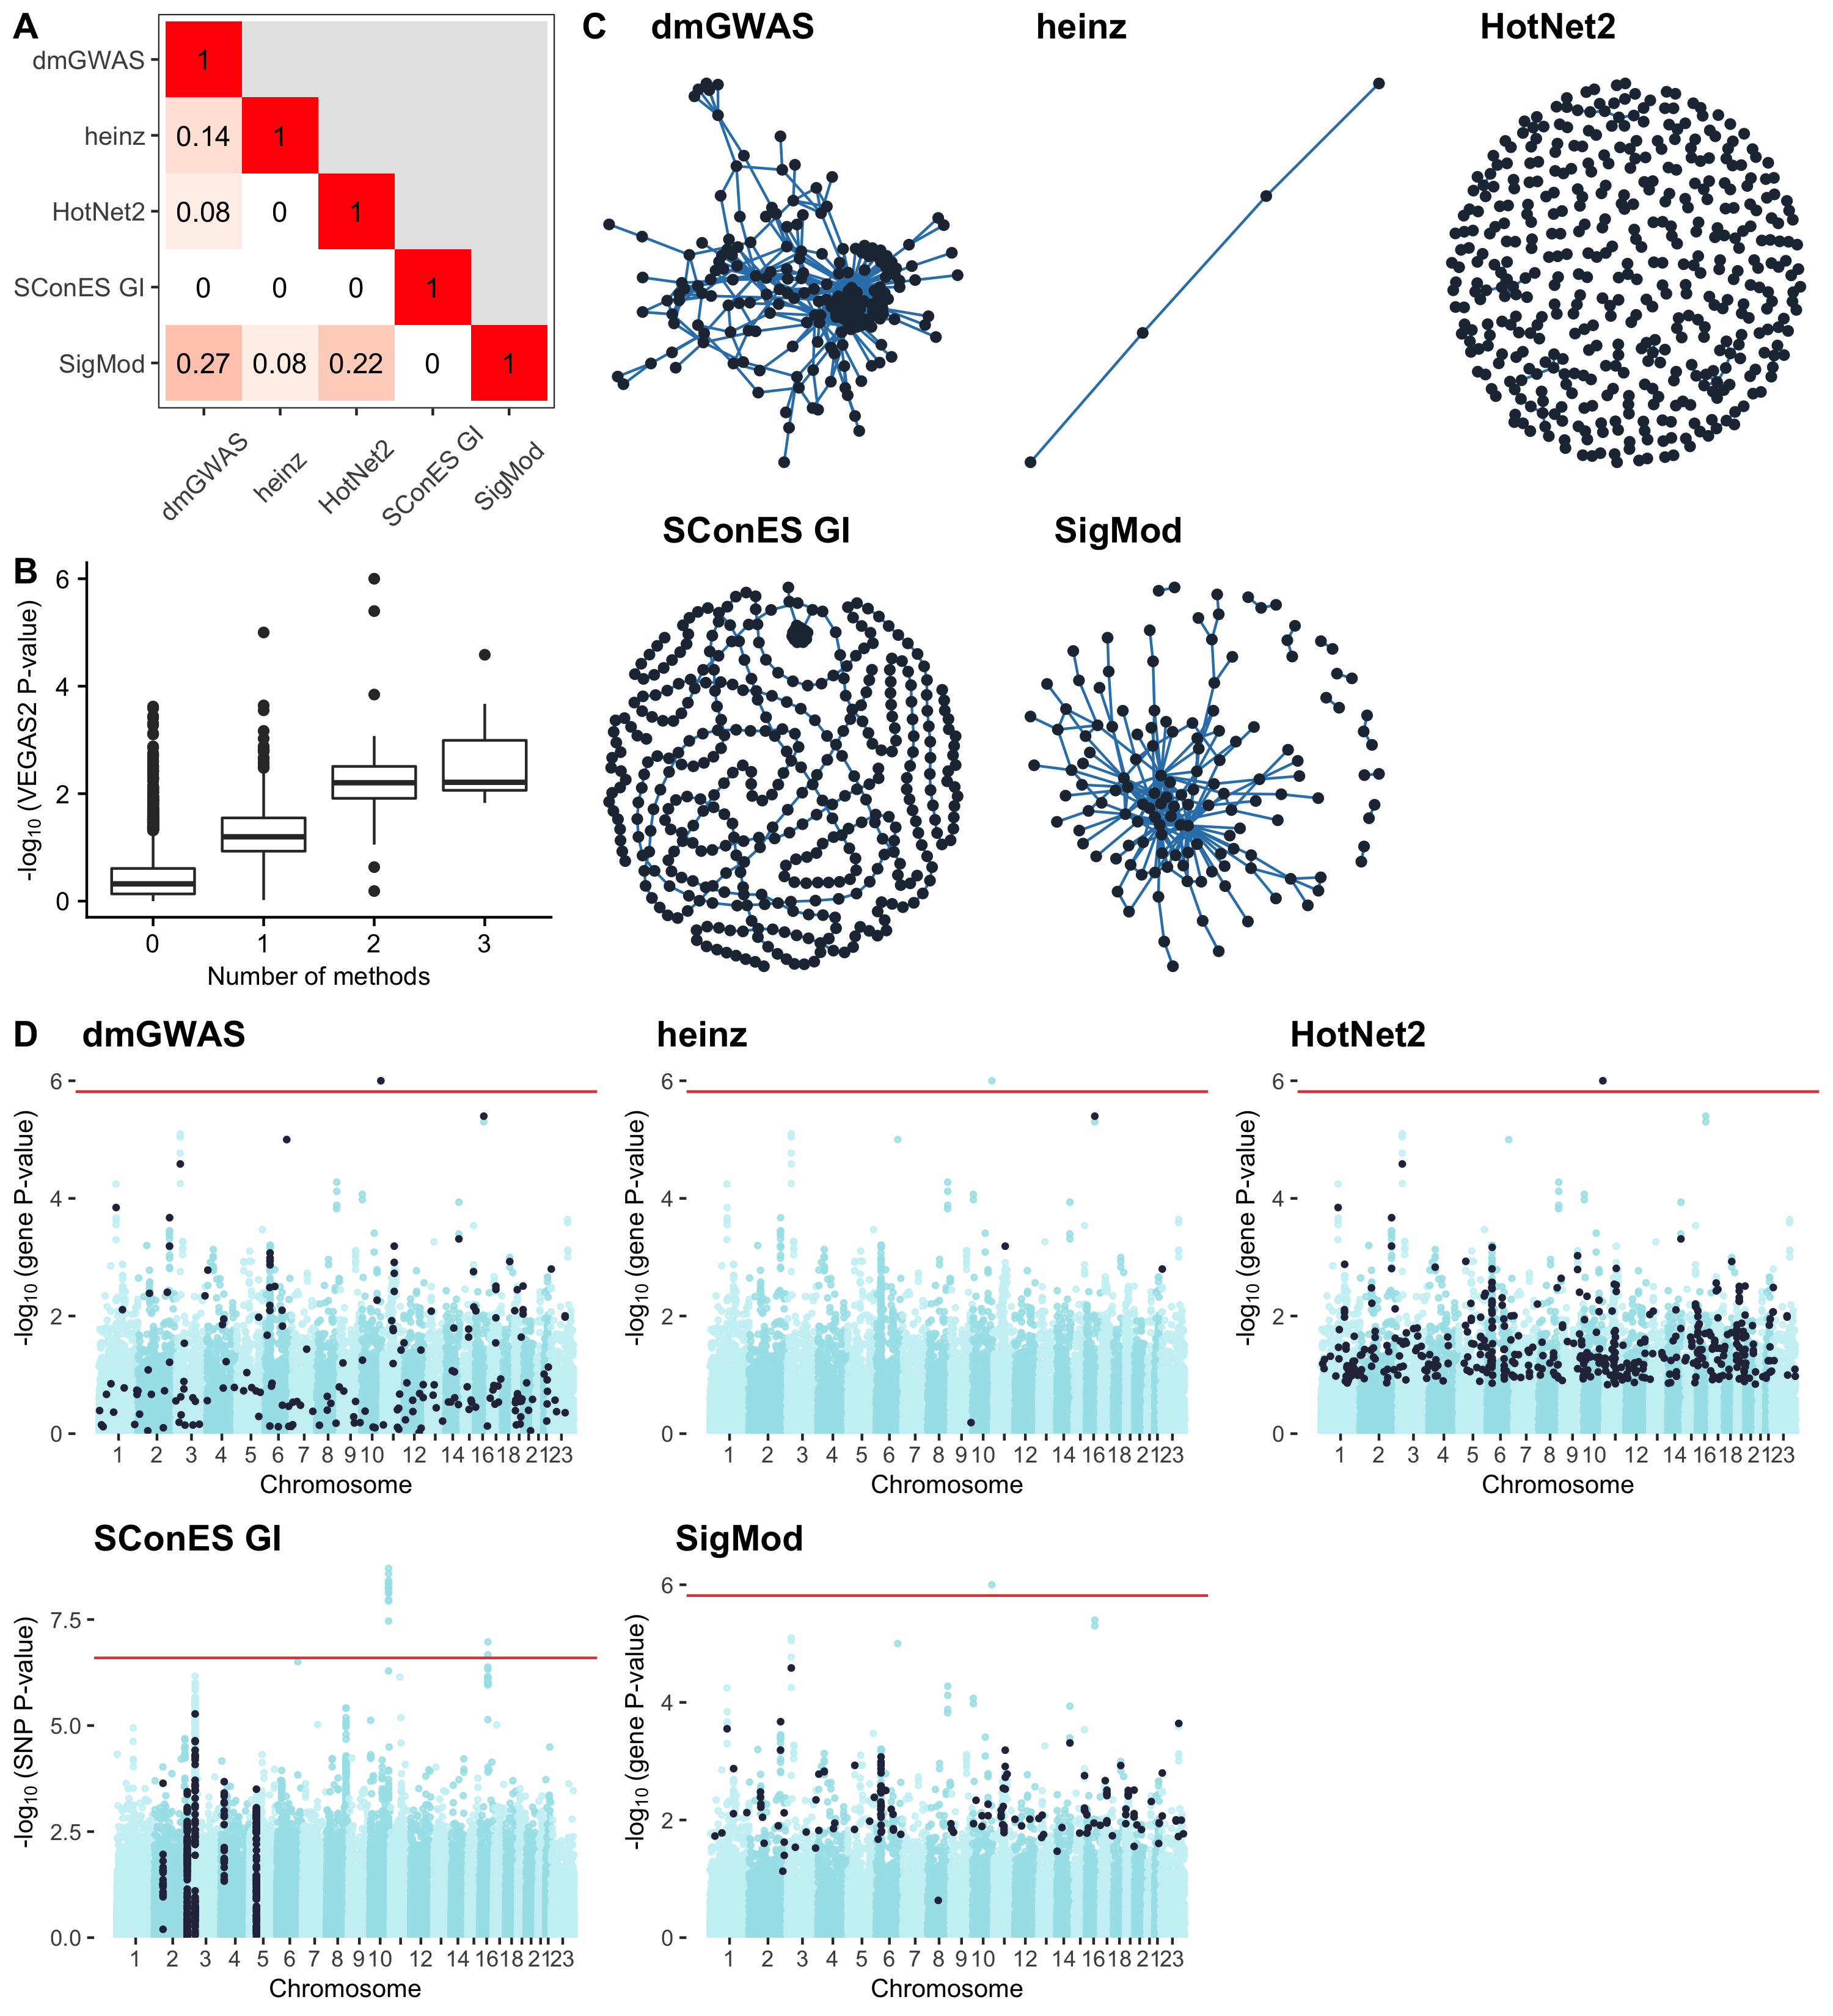
\includegraphics[height=\textwidth]{./figures/figure_1.png}
%DIFDELCMD <   %%%
\DIFdelendFL \DIFaddbeginFL 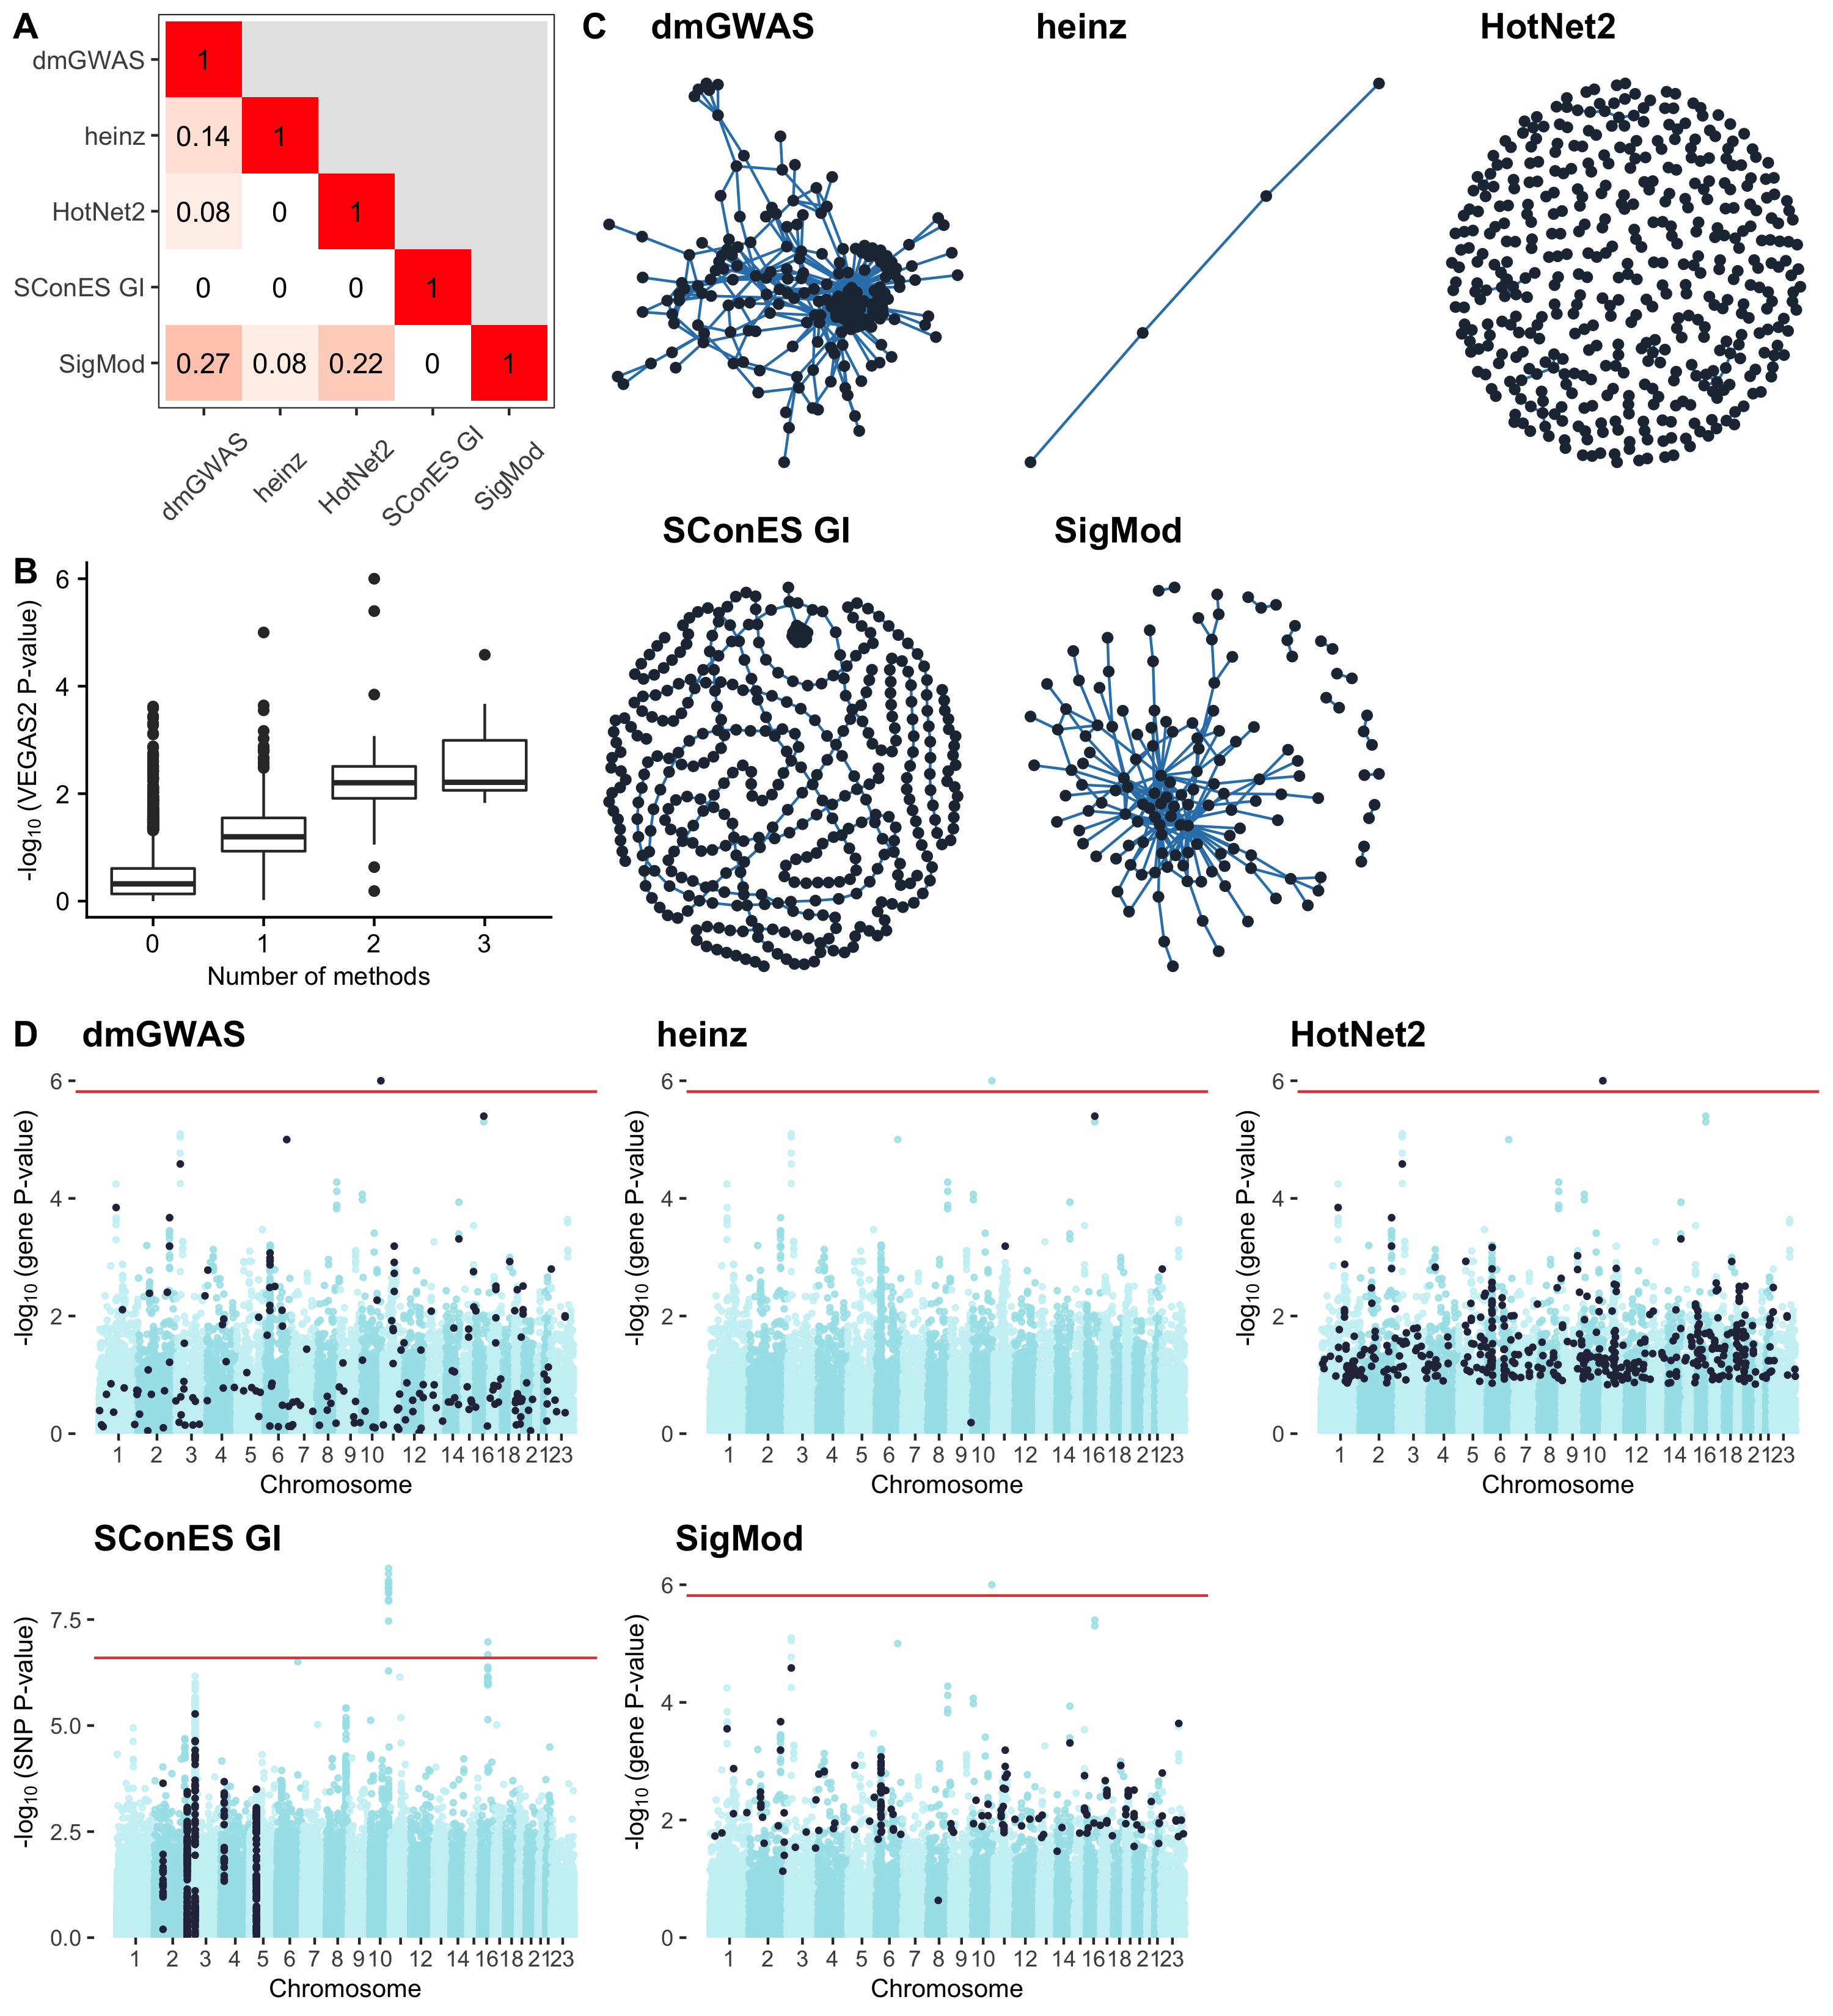
\includegraphics[width=\textwidth]{./figures/figure_1.png}
  \DIFaddendFL \caption{{\bf Overview of the solutions produced by the different network methods (Section~\ref{methods:methods}) on the GENESIS dataset. } As LEAN did not produce any significant \DIFdelbeginFL \DIFdelFL{gene }\DIFdelendFL \DIFaddbeginFL \DIFaddFL{network }\DIFaddendFL (BH adjusted P\=/value~\DIFdelbeginFL \DIFdelFL{<}\DIFdelendFL \DIFaddbeginFL \DIFaddFL{$<$}\DIFaddendFL ~0.05), it was excluded. Unless indicated otherwise, results refer to genes, except for SConES GI which are at the SNP-level. \textbf{(A)}\DIFaddbeginFL \DIFaddFL{~Overlap between the genes selected by each of the methods, measured by Pearson correlation between indicator vectors. }\textbf{\DIFaddFL{(B)}}\DIFaddFL{~VEGAS2 P-values of the genes in the PPIN not selected by any network method (12\,213), and of those selected by 1 (575), 2 (73), or 3 (20) methods. }\textbf{\DIFaddFL{(C)}}\DIFaddFL{~}\DIFaddendFL Manhattan plots of SNPs/genes; in black, the method's solution. The Bonferroni threshold is indicated by a red line (2.54~\texttimes{}~10\textsuperscript{-7} for SNPs, 1.53~\texttimes{}~10\textsuperscript{-6} for genes). \DIFdelbeginFL \textbf{\DIFdelFL{(B)}} %DIFAUXCMD
\DIFdelFL{Overlap between the genes selected by each of the methods, measured by Pearson correlation between indicator vectors. }\textbf{\DIFdelFL{(C)}} %DIFAUXCMD
\DIFdelFL{Precision and recall of the evaluated methods with respect to Bonferroni-significant SNPs/genes in BCAC. For reference, we added a gray line with a slope of 1. }\DIFdelendFL \textbf{(D)}\DIFaddbeginFL \DIFaddFL{~}\DIFaddendFL Solution networks produced by the different methods.}
  \label{fig:solution_overview}
\end{figure}

Despite their differences, there are additional common themes. All obtained \DIFdelbegin \DIFdel{solution subnetworks }\DIFdelend \DIFaddbegin \DIFadd{solutions }\DIFaddend have lower association P\=/values than the whole PPIN (median \DIFaddbegin \DIFadd{VEGAS2 }\DIFaddend P\=/value $\ll 0.46$, Table~\ref{tab:gene_solutions}), despite containing genes with higher P\=/values as well (Fig~\ref{fig:solution_overview}\DIFdelbegin \DIFdel{A}\DIFdelend \DIFaddbegin \DIFadd{D}\DIFaddend ). This exemplifies the trade-off between \DIFdelbegin \DIFdel{statistical significance }\DIFdelend \DIFaddbegin \DIFadd{controlling for type I error }\DIFaddend and biological relevance. However, there are nuances between solutions in this regard: heinz strongly favored genes with lower P\=/values, while dmGWAS was less conservative (median \DIFaddbegin \DIFadd{VEGAS2 }\DIFaddend P\=/values 0.0012 and 0.19, respectively); SConES tended to select whole LD-blocks; and HotNet2 and SigMod were less likely to select low scoring genes. Additionally, the \DIFdelbegin \DIFdel{solution subnetworks }\DIFdelend \DIFaddbegin \DIFadd{solutions }\DIFaddend presented other desirable properties. First, five of them were enriched in known breast cancer susceptibility genes (consensus, dmGWAS, heinz, HotNet2, and SigMod, Fisher's exact test one-sided P\=/value\DIFdelbegin \DIFdel{< }\DIFdelend \DIFaddbegin \DIFadd{$<$}\DIFaddend 0.03). Second, the genes in four \DIFdelbegin \DIFdel{solution subnetworks }\DIFdelend \DIFaddbegin \DIFadd{solutions }\DIFaddend displayed on average a higher betweenness centrality than the rest of the genes, a difference that is significant in four solutions (consensus, dmGWAS, HotNet2, and SigMod, Wilcoxon rank-sum test P\=/value\DIFdelbegin \DIFdel{< }\DIFdelend \DIFaddbegin \DIFadd{$<$}\DIFaddend 1.4 \texttimes{} 10\textsuperscript{-21}). This agrees with the notion that disease genes are more central than other non-essential genes \cite{pinero_uncovering_2016}, an observation that holds in breast cancer (one-tailed Wilcoxon rank-sum test P\=/value~=~2.64 \texttimes{} 10\textsuperscript{-5} when comparing the betweenness of known susceptibility genes versus the rest). Interestingly, SConES selected SNPs that are also more central than the average SNP (\DIFdelbegin \DIFdel{Supplementary table~}\DIFdelend \nameref{stab:snp_solutions}), suggesting that causal SNPs are also more central than \DIFdelbegin \DIFdel{non associated }\DIFdelend \DIFaddbegin \DIFadd{non-associated }\DIFaddend SNPs.

\subsection{A case study: the consensus \DIFdelbegin \DIFdel{network}\DIFdelend \DIFaddbegin \DIFadd{solution}\DIFaddend }
\label{results:consensus}

Despite \DIFdelbegin \DIFdel{the heterogeneity of the solutions, }\DIFdelend their shared properties\DIFaddbegin \DIFadd{, the differences between the solutions of the different methods }\DIFaddend suggest that each \DIFdelbegin \DIFdel{method }\DIFdelend \DIFaddbegin \DIFadd{of them }\DIFaddend captures different aspects of cancer susceptibility. Indeed, \DIFdelbegin \DIFdel{only 20 genes are common to more than twosolutions (}%DIFDELCMD < \nameref{sfig:consensus_stats}%%%
\DIFdel{A), but encouragingly, }\DIFdelend \DIFaddbegin \DIFadd{out of the 668 genes that are selected by at least one method, only 93 are selected by at least two, 20 by three, and none by four or more. Encouragingly, }\DIFaddend the more methods selected a gene, the higher its association score to the phenotype (\DIFdelbegin %DIFDELCMD < \nameref{sfig:consensus_stats}%%%
\DIFdel{B). To }\DIFdelend \DIFaddbegin \DIFadd{Fig \ref{fig:solution_overview}B), a relationship that plateaus at 2. Hence, to }\DIFaddend leverage on their strengths and compensate their respective weaknesses, we built a consensus \DIFdelbegin \DIFdel{subnetwork }\DIFdelend \DIFaddbegin \DIFadd{solution }\DIFaddend that captures the \DIFdelbegin \DIFdel{mechanisms most shared among the solution subnetworks }\DIFdelend \DIFaddbegin \DIFadd{genes shared among at least two solutions }\DIFaddend (Section~\ref{methods:methods}). This \DIFdelbegin \DIFdel{subnetwork }\DIFdelend \DIFaddbegin \DIFadd{solution }\DIFaddend (Fig~\ref{fig:consensus}) contains 93 genes and exhibits the aforementioned properties of the individual solutions: enrichment in breast cancer susceptibility genes and higher betweenness centrality than the rest of the genes. 

\begin{figure}[!ht]
  \centering
  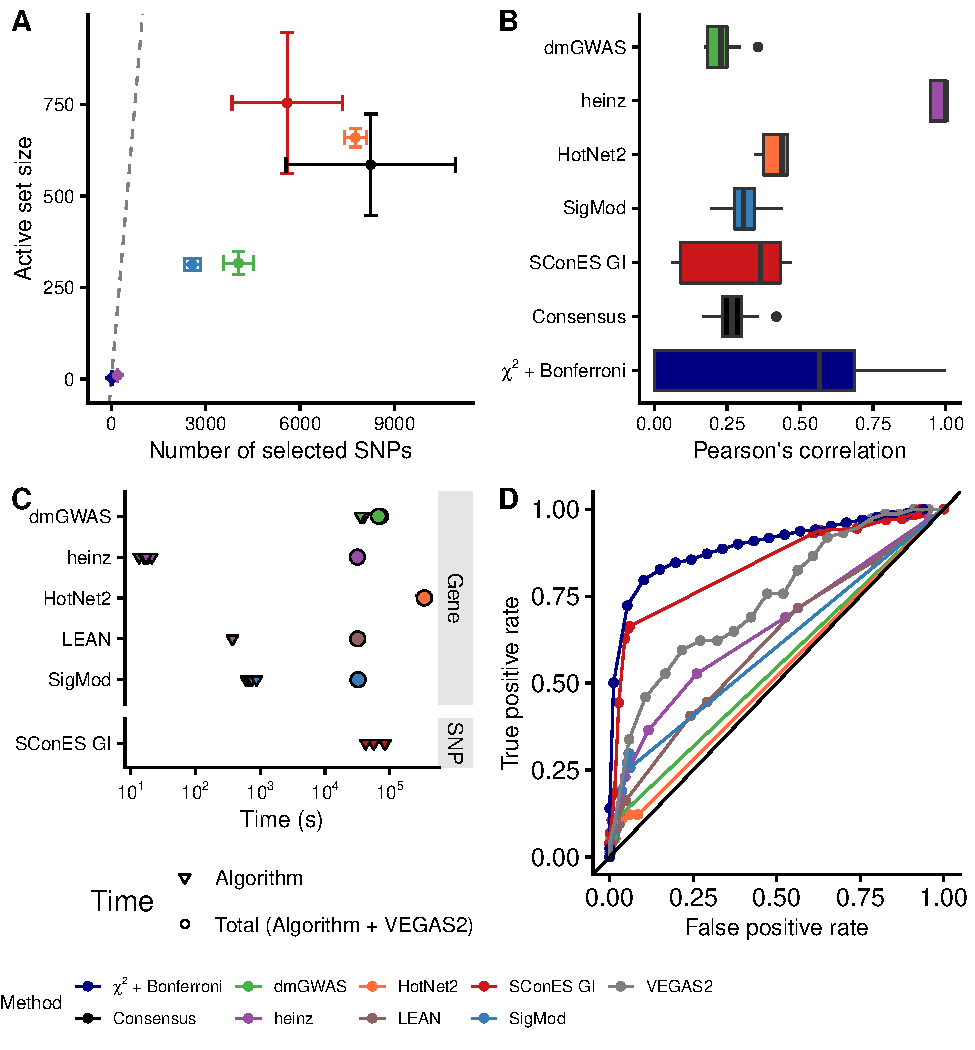
\includegraphics[width=.7\linewidth]{./figures/figure_3.pdf}
  \caption{ {\bf Consensus \DIFdelbeginFL \DIFdelFL{subnetwork }\DIFdelendFL \DIFaddbeginFL \DIFaddFL{solution }\DIFaddendFL on GENESIS (Section~\ref{methods:methods}) }. Each node is represented by a pie chart, which shows the methods that selected it. We labeled (and enlarged) the two most central genes (\emph{COPS5} and \emph{OFD1}) and those genes that are known breast cancer susceptibility genes and/or significantly associated with breast cancer susceptibility in the BCAC dataset \DIFaddbeginFL \DIFaddFL{(Section~\ref{methods:bcac})}\DIFaddendFL . The latter ones are also colored in pink. All gene names are indicated in \nameref{sfig:consensus-names}.}
  \label{fig:consensus}
\end{figure}

A pathway enrichment analysis of the genes in the consensus \DIFdelbegin \DIFdel{network }\DIFdelend \DIFaddbegin \DIFadd{solution }\DIFaddend also shows similar pathways as the individual solutions \DIFaddbegin \DIFadd{(}\nameref{stab:consensus_pwy}\DIFadd{)}\DIFaddend . We found two involved mechanisms: \emph{mitochondrial translation} and \emph{attenuation phase}. The former is supported by genes like \emph{MRPS30} (VEGAS2 P\=/value~=~0.001), which encode a mitochondrial ribosomal protein and was also linked to breast cancer susceptibility \cite{quigley_5p12_2014}. Interestingly, increased mitochondrial translation has been found in cancer cells \cite{Yu2016Repositioning}, and its inhibition proposed as a therapeutic target. With regards to \DIFaddbegin \DIFadd{the }\DIFaddend attenuation phase of heat shock response, it involves three Hsp70 chaperones: HSPA1A, HSPA1B, and HSPA1L. The genes encoding these proteins are all near each other at 6p21, in the region known as HLA. In fact, out of the 22 SNPs that map to any of these three genes, 9 map to all of them, and 4 to two, making \DIFaddbegin \DIFadd{it }\DIFaddend hard to disentangle their effects. \emph{HSPA1A} was the most strongly associated gene (VEGAS2 P\=/value~=~8.37~\texttimes{}~10\textsuperscript{-4}).  

Topologically the consensus consists of a connected component composed of 49 genes, and multiple smaller subnetworks. Among the latter, 19 genes are in subnetworks containing a single gene or two connected nodes, implying that they do not have a consistently altered neighborhood, but are strongly associated themselves and hence picked by at least two methods. \DIFdelbegin \DIFdel{The opposite would be the case of highly central genes }\DIFdelend \DIFaddbegin \DIFadd{In the former we find some genes that are highly central }\DIFaddend in the PPIN, a property which is weakly anti-correlated with the P\=/value of association to the disease (Pearson correlation coefficient~=~-0.26, \nameref{sfig:consensus_stats}\DIFdelbegin \DIFdel{D}\DIFdelend ). This suggests that \DIFdelbegin \DIFdel{they }\DIFdelend \DIFaddbegin \DIFadd{these genes }\DIFaddend were selected because they were on the shortest path between \DIFaddbegin \DIFadd{another }\DIFaddend two highly associated genes. In view of this, we hypothesize that highly central genes might contribute to the heritability through alterations of their neighborhood, consistently with the omnigenic model of disease \cite{boyle_expanded_2017}. For instance, the most central node in the consensus \DIFdelbegin \DIFdel{network }\DIFdelend \DIFaddbegin \DIFadd{solution }\DIFaddend is COPS5, a component of the COP9 signalosome which regulates multiple \DIFdelbegin \DIFdel{signalling }\DIFdelend \DIFaddbegin \DIFadd{signaling }\DIFaddend pathways. \emph{COPS5} is related to multiple hallmarks of cancer and is overexpressed in multiple tumors, including breast and ovarian cancer \cite{liu_jab1_cops5_2018}. Despite its lack of association in GENESIS or BCAC (VEGAS2 P\=/value of 0.22 and 0.14 respectively), its neighbors in the consensus \DIFdelbegin \DIFdel{subnetwork }\DIFdelend \DIFaddbegin \DIFadd{solution }\DIFaddend have consistently low P\=/values (median VEGAS2 P\=/value~=~0.006).

\subsection{Network methods boost \DIFdelbegin \DIFdel{biomarker }\DIFdelend discovery}
\DIFaddbegin \label{results:boost}

\DIFaddend 

We compared the results of different network methods to the European sample of the Breast Cancer Association Consortium (BCAC) \cite{Michailidou2017}, the largest GWAS to date on breast cancer (Section~\ref{methods:bcac}). Although BCAC case-control studies do not necessarily target cases with a family history of breast cancer, this comparison is pertinent since we expect a shared genetic architecture at the gene level, at which most network \DIFdelbegin \DIFdel{metods }\DIFdelend \DIFaddbegin \DIFadd{methods }\DIFaddend operate. This shared genetic architecture, together with BCAC's scale (90 times more samples than GENESIS) provides a reasonable counterfactual of what we would expect if GENESIS had a larger sample size. We computed a gene association score on BCAC \DIFdelbegin \DIFdel{, in an equivalent way to the one described in Section~\ref{methods:node_score}}\DIFdelend \DIFaddbegin \DIFadd{(Section~\ref{methods:bcac})}\DIFaddend . The solutions provided by the different  network \DIFdelbegin \DIFdel{approaches }\DIFdelend \DIFaddbegin \DIFadd{methods }\DIFaddend overlap significantly with BCAC findings (Fisher's exact test P\=/value \textless~0.019). The gene-based \DIFdelbegin \DIFdel{network }\DIFdelend methods achieve comparable precision (2\%-25\%) and recall (1.3-12.1\%) at recovering BCAC-significant genes (\DIFdelbegin \DIFdel{Fig~\ref{fig:solution_overview}C). Interestingly, while SConES GI at the SNP-level }\DIFdelend \DIFaddbegin \nameref{sfig:additional-benchmarks}\DIFadd{A). interestingly, while scones gi at the snp-level }\DIFaddend achieves a similar recall (8.6\%), it shows a much higher precision (47.3\%).

\subsection{Network methods share limitations}
\DIFaddbegin \label{results:benchmark}

\DIFaddend 

We compared the six network methods in a 5-fold subsampling setting (Section \DIFdelbegin \DIFdel{\ref{methods:comparison}}\DIFdelend \DIFaddbegin \DIFadd{\ref{methods:benchmark}}\DIFaddend ). Specifically, we measured five properties (Fig~\ref{fig:benchmark}): size of the solution\DIFdelbegin \DIFdel{subnetwork}\DIFdelend ; sensitivity and specificity of an L1-penalized logistic regression classifier on the selected SNPs; stability; and computational runtime. The solution size varies greatly between the different methods (Fig~\ref{fig:benchmark}A). Heinz produced the smallest solutions, with an average of 182 selected SNPs \DIFaddbegin \DIFadd{(Section~\ref{methods:snp2gene})}\DIFaddend . The largest solutions came from SConES GI (6\,256.6 SNPs), and dmGWAS (4\,255.0 SNPs). \DIFaddbegin \DIFadd{LEAN did not produce any solution in any of the subsamples. }\DIFaddend To determine whether the selected \DIFdelbegin \DIFdel{SNPs }\DIFdelend \DIFaddbegin \DIFadd{snps }\DIFaddend could be used for patient classification, we computed the performance of the classifier on the \emph{test dataset} (\DIFdelbegin \DIFdel{Fig~\ref{fig:benchmark}}\DIFdelend \DIFaddbegin \nameref{sfig:additional-benchmarks}\DIFaddend B). The different classifiers displayed similarly poor sensitivities and specificities, all in the 0.52 -- 0.56 range. Interestingly, the classifier trained on all the SNPs had a similar performance, despite being the only method aiming only at minimizing prediction error. It should be considered that, although these performances are low, we do not expect to separate cases from controls well using exclusively genetic data \DIFaddbegin \DIFadd{\mbox{%DIFAUXCMD
\cite{deloscamposComplexTraitPredictionEra2018}}\hspace{0pt}%DIFAUXCMD
}\DIFaddend .

\begin{figure}[!ht]
  \centering
  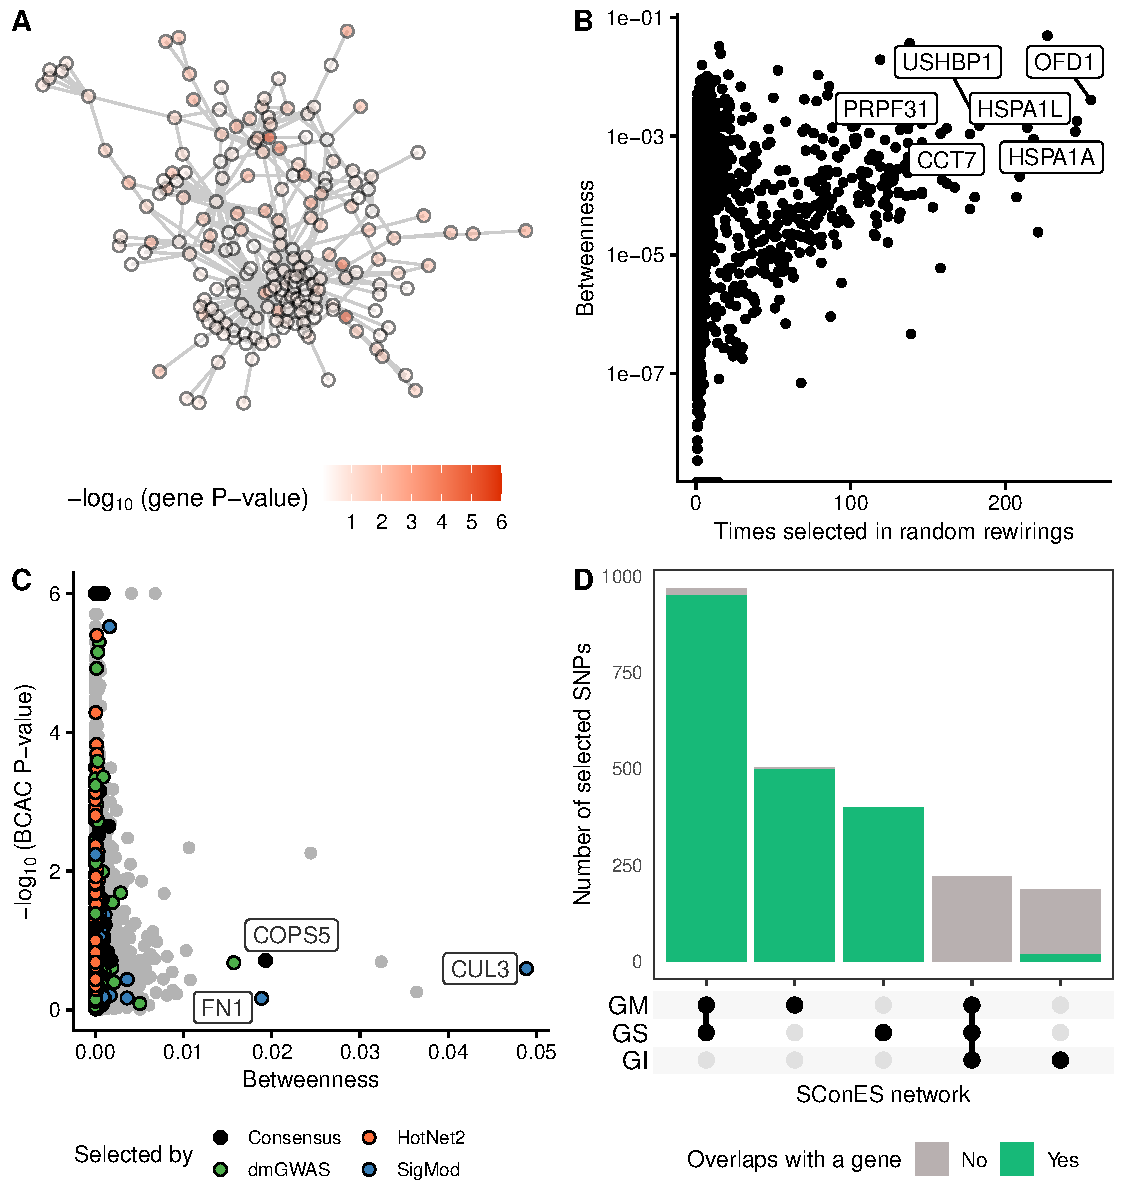
\includegraphics[width=\linewidth]{./figures/figure_4.pdf}
  \caption{{ \bf Comparison of network-based GWAS methods on GENESIS. } Each method was run 5 times on a random subset containing 80\% of the samples, and tested on the remaining samples (Section \DIFdelbeginFL \DIFdelFL{\ref{methods:comparison}}\DIFdelendFL \DIFaddbeginFL \DIFaddFL{\ref{methods:benchmark}}\DIFaddendFL ). As LEAN did not select any gene, it was excluded from all panels except \textbf{D}. \textbf{(A)}\DIFaddbeginFL \DIFaddFL{~}\DIFaddendFL Number of SNPs selected by each method and number of SNPs in the active set found by the classifier\DIFaddbeginFL \DIFaddFL{(Section~\ref{methods:classifier})}\DIFaddendFL . Points are the average over the 5 runs; \DIFdelbeginFL \DIFdelFL{lines }\DIFdelendFL \DIFaddbeginFL \DIFaddFL{the error bars }\DIFaddendFL represent the standard error of the mean. A grey diagonal line with slope 1 is added for comparison\DIFaddbeginFL \DIFaddFL{, indicating the upper bound of the active set (i}\DIFaddendFL .\DIFaddbeginFL \DIFaddFL{e. the number of SNPs in the solution). }\DIFaddendFL For reference, the active set of Lasso using all the SNPs included, on average, 154\,117.4 SNPs. \DIFdelbeginFL \textbf{\DIFdelFL{(B)}} %DIFAUXCMD
\DIFdelFL{Sensitivity and specificity on test set of the L1-penalized logistic regression trained on the features selected by each of the methods. In addition, the performance of the classifier trained on all SNPs is displayed. Points are the average over the 5 runs; lines represent the standard error of the mean. }\DIFdelendFL \textbf{(C)}\DIFaddbeginFL \DIFaddFL{~}\DIFaddendFL Pairwise Pearson correlations of the solutions \DIFdelbeginFL \DIFdelFL{used }\DIFdelendFL \DIFaddbeginFL \DIFaddFL{produced }\DIFaddendFL by different methods. A Pearson correlation of 1 means the two solutions are the same. A Pearson correlation of 0 means that there is no SNP in common between the two solutions. \textbf{(D)}\DIFaddbeginFL \DIFaddFL{~}\DIFaddendFL Runtime of the evaluated methods, by type of network used (\DIFdelbeginFL \DIFdelFL{gene }\DIFdelendFL \DIFaddbeginFL \DIFaddFL{PPIN }\DIFaddendFL or SNP). For \DIFdelbeginFL \DIFdelFL{gene network-based }\DIFdelendFL \DIFaddbeginFL \DIFaddFL{gene-based }\DIFaddendFL methods, inverted triangles represent the runtime of the algorithm itself, and circles the total time, which includes the algorithm themselves and the additional 119\,980 seconds (1 day and 9.33 hours) that VEGAS2 took on average to compute the gene scores from SNP summary statistics.}
  \label{fig:benchmark}
  \end{figure}

Another desirable quality of an algorithm is the stability of the solution with regards to small changes in the input (Section~\ref{methods:algorithm_comparison}). \DIFdelbegin \DIFdel{Both heinz and LEAN displayed a high stability }\DIFdelend \DIFaddbegin \DIFadd{Heinz was high stabile }\DIFaddend in our benchmark, \DIFdelbegin \DIFdel{consistently selecting the same genes and no genes over the 5 subsamples, respectively }\DIFdelend \DIFaddbegin \DIFadd{while the other methods displayed similarly low stabilities }\DIFaddend (Fig~\ref{fig:benchmark}C).\DIFdelbegin \DIFdel{Conversely, the other methods displayed similarly low stabilities. }\DIFdelend 

In terms of computational runtime, the fastest method was heinz (Fig~\ref{fig:benchmark}D), which returned a solution in a few seconds. HotNet2 was the slowest (3 days and 14 hours on average). Including the time required to compute the gene scores, however, slows down considerably gene-based methods; on this benchmark, that step took on average 1 day and 9.33 hours. Considering that, it took 5 days on average for HotNet2 to produce a result.

\subsection{Network topology matters, and might lead to ambiguous results}
\label{results:drawbacks}

As shown above, and despite their similarities, the network methods produced remarkably different solutions. This is due to the \DIFdelbegin \DIFdel{particularities of each methods, and directly or indirectly provide information about the dataset }\DIFdelend \DIFaddbegin \DIFadd{fact that each of them models the optimal solution differently. Importantly, understanding which assumptions they make allows to understand the dataset more deeply}\DIFaddend . For instance, the fact that LEAN did not return any \DIFdelbegin \DIFdel{biomarker }\DIFdelend \DIFaddbegin \DIFadd{gene }\DIFaddend implies that there is no gene such that both itself and its environment are on average strongly associated with the disease.

In \DIFdelbegin \DIFdel{this }\DIFdelend \DIFaddbegin \DIFadd{the GENESIS }\DIFaddend dataset, heinz's solution is very conservative, providing a small solution with the lowest median P\=/value \DIFdelbegin \DIFdel{for the subnetwork }\DIFdelend (Table~\ref{tab:gene_solutions}). \DIFdelbegin \DIFdel{Due to this parsimonious and highly associated solution, it was the best method to stably select a set of biomarkers }\DIFdelend \DIFaddbegin \DIFadd{By repeatedly selecting this compact solution, heinz was the most stable method }\DIFaddend (Fig~\ref{fig:benchmark}C). Its conservativeness stems from its preprocessing step, which models the gene P\=/values as a mixture model of a beta distribution and a uniform distribution, controlled by an FDR parameter. Due to the limited signal at the gene level in this dataset (\nameref{sfig:snp_gene_manhattan}B), only 36 of all the genes retain a positive score after that transformation. Yet, this small solution does not provide much insight into the susceptibility mechanisms to cancer. Importantly, it ignores genes that are associated to cancer in this dataset like \emph{FGFR2}. 

On the other end of the spectrum, dmGWAS, HotNet2, and SigMod produced large solutions. dmGWAS' \DIFdelbegin \DIFdel{subnetwork is the least associated subnetwork }\DIFdelend \DIFaddbegin \DIFadd{solution is the lowest scoring solution }\DIFaddend on average. This is due to the greedy framework it uses, which has a bias for larger solutions \cite{nikolayeva_network_2018}. It considered all nodes at distance 2 of the examined subnetwork, and accepted a weakly associated \DIFdelbegin \DIFdel{genes }\DIFdelend \DIFaddbegin \DIFadd{gene }\DIFaddend if it was linked to another, \DIFdelbegin \DIFdel{strongly associated }\DIFdelend \DIFaddbegin \DIFadd{high scoring }\DIFaddend one. This is exacerbated when the results of successive greedy searches are aggregated, leading to a large, tightly connected cluster of unassociated genes (Fig~\ref{fig:issues}A). This relatively low signal-to-noise ratio combined with the large solution requires additional analyses to draw conclusions, such as enrichment analyses. In the same line, HotNet2's \DIFdelbegin \DIFdel{subnetwork }\DIFdelend \DIFaddbegin \DIFadd{solution }\DIFaddend is even harder to interpret, being composed of 440 genes divided into 135 subnetworks. Lastly, SigMod misses some of the \DIFdelbegin \DIFdel{most strongly associated}\DIFdelend \DIFaddbegin \DIFadd{highest scoring}\DIFaddend , breast cancer susceptibility genes in the dataset, like \emph{FGFR2} and \emph{TOX3}.

\begin{figure}[!ht]
  \centering
  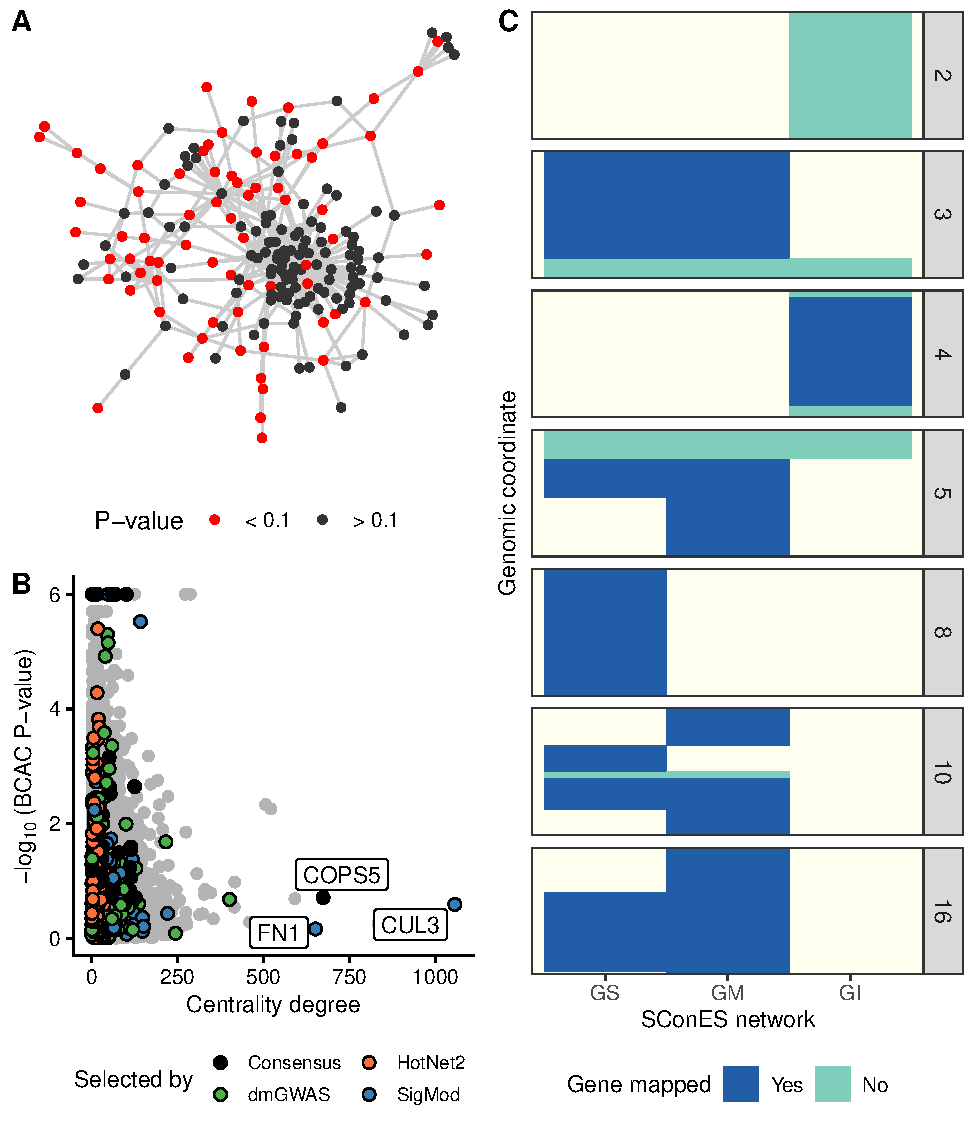
\includegraphics[width=\linewidth]{./figures/figure_2.pdf}
  \caption{{\bf Drawbacks encountered when using network \DIFdelbeginFL \DIFdelFL{guided }\DIFdelendFL methods.} \textbf{(A)}~DmGWAS solution\DIFdelbeginFL \DIFdelFL{subnetwork. Genes }\DIFdelendFL \DIFaddbeginFL \DIFaddFL{, }\DIFaddendFL with \DIFdelbeginFL \DIFdelFL{a }\DIFdelendFL \DIFaddbeginFL \DIFaddFL{the genes colored according to the -log$_{10}$ of their }\DIFaddendFL P\=/value\DIFdelbeginFL \DIFdelFL{< 0.1 are highlighted in red}\DIFdelendFL . \textbf{(B)}~Centrality degree and -log\textsubscript{10} of the VEGAS2 P\=/value in BCAC for each of the nodes in the PPIN. We highlighted the genes selected by each method, and the ones selected by more than one (``Consensus''). We labeled the three most central genes that were picked by any method. \textbf{(C)}~\DIFaddbeginFL \DIFaddFL{Number of times a gene was selected by either dmGWAS, heinz, LEAN, or SigMod in 100 rewirings of the PPIN (Section~\ref{methods:pathway_enrichment}) and its centrality degree. }\textbf{\DIFaddFL{(D)}}\DIFaddFL{~}\DIFaddendFL Overlap between the solutions of SConES GS, GM or GI in the different genomic regions. SNPs that were not selected in the studied network, but were selected in another one, are displayed in background color. }
  \label{fig:issues}
  \end{figure}

Another peculiarity of network methods is their relationship to degree centrality. \DIFdelbegin \DIFdel{On the one hand we observed that highly central genes often had no association to disease (Fig~\ref{fig:issues}B). On the other}\DIFdelend \DIFaddbegin \DIFadd{We studied randomly rewirings of the PPIN while preserving node centrality (Section~\ref{methods:rewiring}). In this setting}\DIFaddend , network methods \DIFdelbegin \DIFdel{favor }\DIFdelend \DIFaddbegin \DIFadd{favored }\DIFaddend central genes, as they often connect high scoring nodes \DIFdelbegin \DIFdel{. This }\DIFdelend \DIFaddbegin \DIFadd{(Fig~\ref{fig:issues}B). This is despite the fact that highly central genes often had no association to breast cancer susceptibility (Fig~\ref{fig:issues}C). This }\DIFaddend was specially the case of SigMod, which selected three highly central, unassociated genes: \emph{COPS5}, \emph{CUL3} and \emph{FN1}. As we showed in Section \ref{results:consensus}, and will show in \ref{results:stable-consensus}, there is evidence in the literature of the contribution of the first two to breast cancer susceptibility. With regards to \emph{FN1}, it encodes a fibronectin, a protein of the extracellular matrix involved in cell adhesion and migration. Overexpression of \emph{FN1} has been observed in breast cancer \cite{Ioachim2002}, and it is negatively correlated with poor prognosis in other cancer types \cite{Yi2016,Sponziello2016}.

By virtue of using a SNP subnetwork, SConES analyzes each SNP in their functional context. It therefore can select SNPs in genes without any associated interactor, as well as SNPs in non-coding regions or in non-interacting genes. \DIFdelbegin \DIFdel{In fact, due to linkage disequilibrium, SConES favors such genes, as selecting SNPs in an LD-block which overlaps with a gene favors selecting the rest of the gene. This might explain why }\DIFdelend \DIFaddbegin \DIFadd{We compared the solution of SConES in the GI network (using PPIN information), to the one using only positional information (GS network), or positional and gene annotations (GM network). Importantly, }\DIFaddend SConES produces similar results on the GS and GM networks \DIFdelbegin \DIFdel{, heavily affected by linkage disequilibrium }\DIFdelend (\nameref{sfig:pearson_methods}). \DIFdelbegin \DIFdel{On the other hand, SConES penalizes selecting SNPs and not their neighbors. This makes it conservative regarding SNPs with many interactions, like those mapped to hub genes in the PPIN. For this reason, SConES GIdid not select any protein coding gene, despite selecting similar regions as SConES GS }\DIFdelend \DIFaddbegin \DIFadd{While the solutions on those two greatly overlap with SConES GI's, they contain additional gene-coding segments }\DIFaddend (Fig~\ref{fig:issues}C). In fact \DIFdelbegin \DIFdel{SConES GS and SConES GM select }\DIFdelend \DIFaddbegin \DIFadd{the formers' solutions are chromosome }\DIFaddend regions related to breast cancer, like 3p24 (\emph{SLC4A7}/\emph{NEK10} \cite{ahmed_newly_2009}), 5p12 (\emph{FGF10}, \emph{MRPS30} \cite{quigley_5p12_2014}), 10q26 (\emph{FGFR2}), and 16q12 (\emph{TOX3}). On top of those SConES GS selects region 8q24 (\emph{POU5F1B} \cite{breyer_expressed_2014}). 

\DIFdelbegin \DIFdel{We hypothesize that the lack of results on the PPIN network of SConES GI and LEAN are due to the same cause: the absence of joint association of a gene and a majority of its neighbors. Although in the case of SConES other hyperparameters could lead to a more informative solution (e.g. a lower \(\lambda\) in Equation~\ref{eq:scones}), it is unclear what the best strategy to find them is. In addition, due to the design of the iCOGS array, the genome of GENESIS participants has not been unbiasedly surveyed: some regions are fine-mapped --- which might distort gene structure in GM and GI networks --- while others are under studied --- hindering the accuracy with which the GS network captures the genome structure.}\DIFdelend 

 
\subsection{Adjusting for instability preserves global network properties}
\label{results:stable-consensus}

Most of the network methods, including the consensus, were highly unstable, raising questions about the reliability of the results. We built a new, stable consensus \DIFdelbegin \DIFdel{network }\DIFdelend \DIFaddbegin \DIFadd{solution }\DIFaddend using the genes selected most often across the 30 solutions obtained by running the 6 methods on 5 different splits of the data (Section \DIFdelbegin \DIFdel{\ref{methods:comparison}}\DIFdelend \DIFaddbegin \DIFadd{\ref{methods:benchmark}}\DIFaddend ). Such a network is expected to capture the subnetworks more often found altered, and hence should be more resistant to noise. We used only genes selected in at least 7 of the solutions, which corresponded to 1\% of all genes selected at least once. The resulting \DIFdelbegin \DIFdel{stablility-based }\DIFdelend \DIFaddbegin \DIFadd{stability-based }\DIFaddend consensus was composed of 68 genes (Fig \ref{fig:stable-consensus}). This network shares most of the \DIFdelbegin \DIFdel{proterties }\DIFdelend \DIFaddbegin \DIFadd{properties }\DIFaddend of the consensus: breast cancer susceptibility genes are overrepresented (P\=/value = 3 \texttimes{} 10\textsuperscript{-4}), as well as genes involved in mitochondrial translation and the attenuation phase (adjusted P\=/values 0.001 and 3 \texttimes{} 10\textsuperscript{-5} respectively); the selected genes are more central than average (P\=/value = 1.1 \texttimes{} 10\textsuperscript{-14}); and a considerable number of nodes (19) are isolated.

\begin{figure}[!ht]
  \centering
  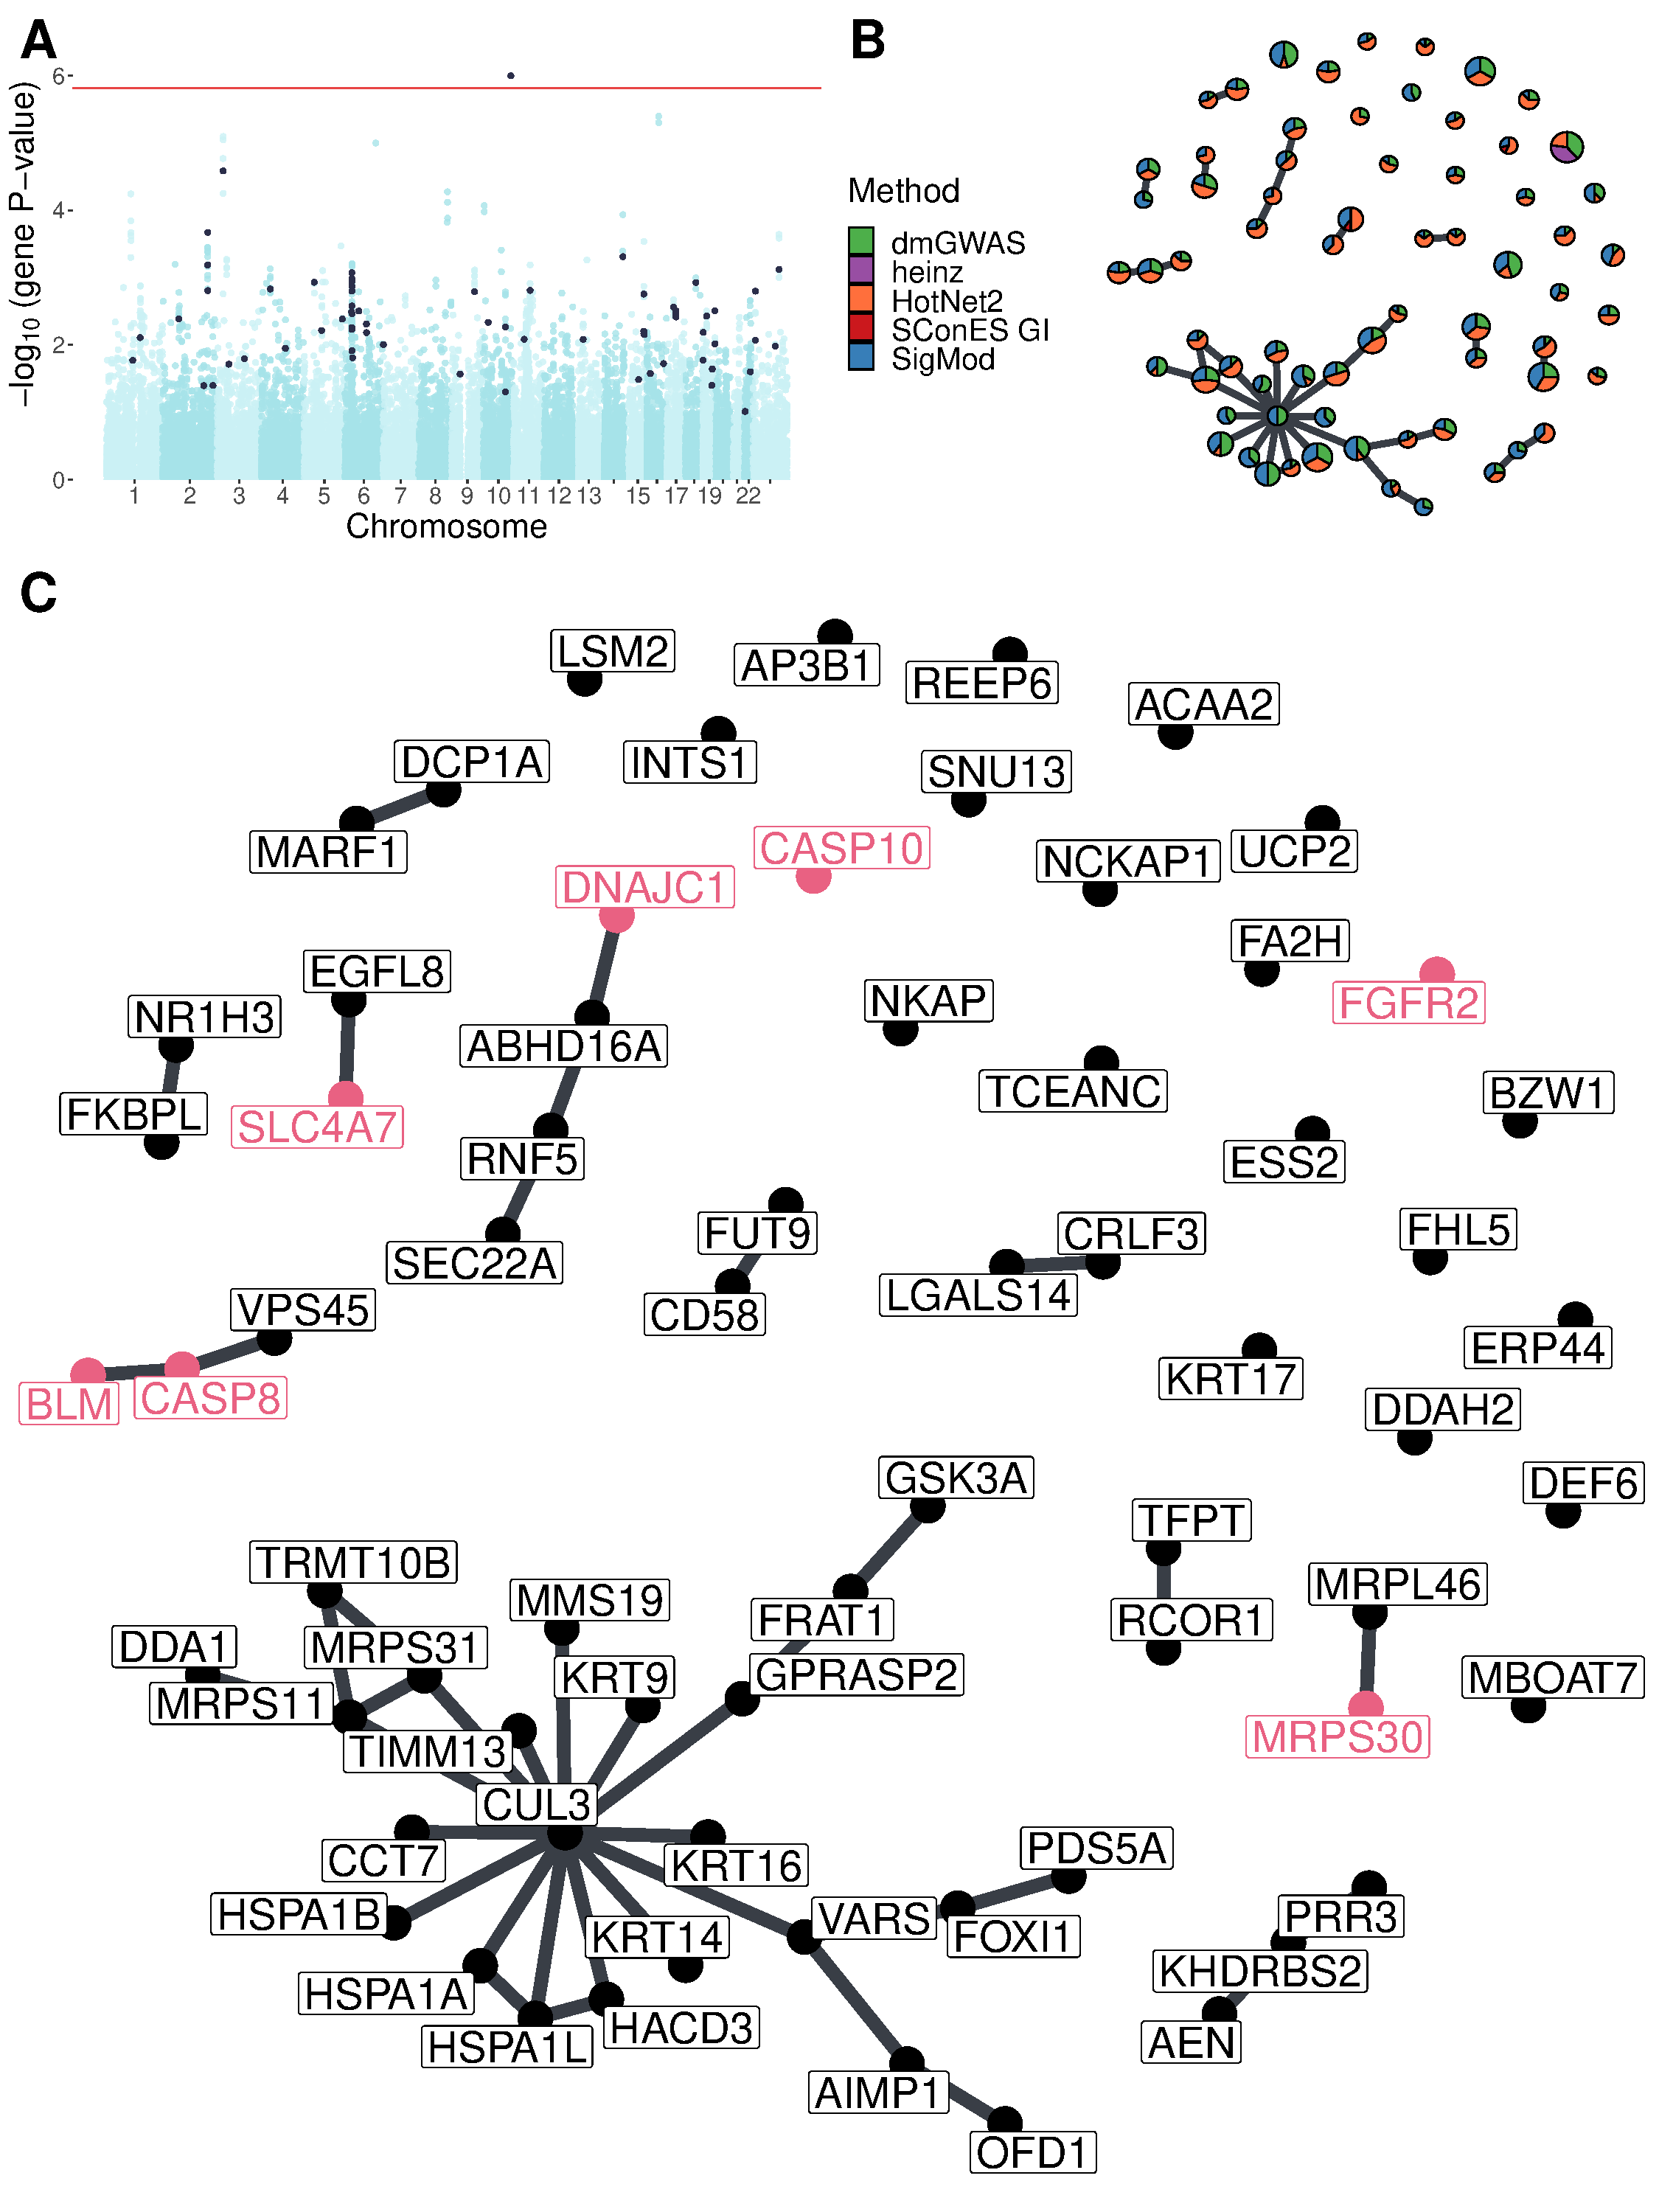
\includegraphics[width=.7\linewidth]{./figures/figure_5.pdf}
  \caption{{\bf Stable consensus \DIFdelbeginFL \DIFdelFL{subnetwork }\DIFdelendFL \DIFaddbeginFL \DIFaddFL{solution }\DIFaddendFL on GENESIS (Section~\ref{results:stable-consensus}).} Each node is represented by a pie chart, which shows the methods that selected it. We labeled (and enlarged) the most central genes (\emph{CUL3}) and those genes that are known breast cancer susceptibility genes and/or significantly associated with breast cancer susceptibility in the BCAC dataset \DIFaddbeginFL \DIFaddFL{(Section~\ref{methods:bcac})}\DIFaddendFL . The latter ones are also colored in pink. All gene names are indicated in \nameref{sfig:stable-consensus-names}.}
  \label{fig:stable-consensus}
  \end{figure}

\DIFdelbegin \DIFdel{However, although this new network exhibits similar global properties as the previous one, the lack of stability results in different genesbeing selected}\DIFdelend \DIFaddbegin \DIFadd{Despite these similarities, the consensus and the stable consensus solutions include different genes}\DIFaddend . In this case, the most central gene is \emph{CUL3}, which is absent from the previous consensus \DIFdelbegin \DIFdel{network }\DIFdelend \DIFaddbegin \DIFadd{solution }\DIFaddend and has a low association score in both GENESIS and BCAC (P\=/values of 0.04 and 0.26, respectively). This gene is a component of Cullin-RING ubiquitin ligases. Encouragingly, it impacts the protein levels of multiple genes relevant for cancer progression \cite{Chen2016}, and its overexpression was also linked to increased sensitivity to carcinogens \cite{Loignon2009}.

\section{Discussion}

In recent years, the ability of GWAS to unravel the mechanisms leading to complex diseases has been called into question \cite{boyle_expanded_2017}. On the one hand, the omnigenic model proposes that gene functions are interwoven with each other in a dense co-function network. The practical consequence is that larger and larger GWAS will lead to the discovery of an uninformative wide-spread pleiotropy. On the other hand, discovery in GWAS is hindered by a conservative statistical framework. Network methods tackle these two issues by using both the association score and an interaction network to take into consideration the biological context of each of the genes and SNPs. Based on what could be considered diverse interpretations of the omnigenic model, several methods for network-guided \DIFdelbegin \DIFdel{biomarker }\DIFdelend discovery have been proposed in recent years. In this article we evaluated the relevance of six of them by examining \DIFaddbegin \DIFadd{GENESIS, }\DIFaddend a GWAS dataset on familial breast cancer.

\DIFdelbegin \DIFdel{Most of the network methods produced a relevant subset of biomarkers, recapitulating }\DIFdelend \DIFaddbegin \DIFadd{DmGWAS, Heinz, HotNet2, SConES and SigMod relevant solutions, which recapitulate }\DIFaddend known breast cancer susceptibility genes. In general, the selected genes and SNPs were more central than average, in accordance with the observation that disease genes are more relatively central \cite{pinero_uncovering_2016}. However, very central nodes are also more likely to be connecting any given random pair of nodes, making them more likely to be selected by \DIFdelbegin \DIFdel{these network methods . Across }\DIFdelend \DIFaddbegin \DIFadd{network methods (Section \ref{results:drawbacks}). Yet, across }\DIFaddend this article we show that highly central genes that were selected (\emph{COPS5}, \emph{CUL3} and \emph{FN1}) could plausibly be involved in breast cancer susceptibility. \DIFdelbegin \DIFdel{Yet, further work is needed to characterize the impact of centrality on network methods' outputs. }\DIFdelend Despite these similarities, the solutions \DIFaddbegin \DIFadd{of the methods }\DIFaddend were notably different. At one end of the spectrum, SConES and heinz preferred small, highly associated solutions, \DIFdelbegin \DIFdel{providing a conveniently short list of biomarkers, }\DIFdelend at the expense of not shedding much light on the etiology of the disease. On the other end, SigMod and dmGWAS gravitate towards larger, less associated solutions which provide a wide overview of the biological context. While this deepens our understanding of the disease and \DIFdelbegin \DIFdel{provide }\DIFdelend \DIFaddbegin \DIFadd{provides }\DIFaddend biological hypotheses, they require further analyses, which might deter unexperienced practitioners. \DIFaddbegin \DIFadd{For instance, examining the network properties of the genes in the solution (e.g. centrality and neighbors). Those might drive the selection of genes, especially of those with low association scores. }\DIFaddend HotNet2 balances both approaches at the expense of producing the largest solution: a constellation of many, highly associated, small subnetworks. Additionally, all solutions share two drawbacks. First, they are all equally bad at discriminating cases from controls. Yet, the classification accuracy of network methods is similar to that of a machine learning classifier, which suggests that cases and controls are difficult to separate in \DIFdelbegin \DIFdel{this }\DIFdelend \DIFaddbegin \DIFadd{the GENESIS }\DIFaddend dataset. This might be due to unaccounted for environmental factors, and limited statistical power, which reduces the ability to identify relevant SNPs. Second, all methods are remarkably unstable, yielding different solutions for slightly different inputs. This might partly be caused by the instability of the P\=/values themselves in low statistical power settings \cite{halseyFickleValueGenerates2015}. Hence, heinz's conservative transformation of P\=/values, which favors only the most extreme ones, leads to improved stability. Another source of instability might be the redundancy inherent to biological networks\DIFdelbegin \DIFdel{.}\DIFdelend \DIFaddbegin \DIFadd{, since they are subject to an evolutionary pressure to avoid single points of failure \mbox{%DIFAUXCMD
\cite{wagnerAlternativeRoutesMutational2007}}\hspace{0pt}%DIFAUXCMD
. Hence, often network methods will have multiple paths connecting two high-scoring nodes.}\DIFaddend 

To overcome the limitations of the individual methods while exploiting their strengths, we proposed combining them into a consensus \DIFdelbegin \DIFdel{subnetwork}\DIFdelend \DIFaddbegin \DIFadd{solution}\DIFaddend . We use a straightforward strategy of including any node that was recovered by multiple methods. We proposed two networks: a consensus \DIFdelbegin \DIFdel{network }\DIFdelend \DIFaddbegin \DIFadd{solution }\DIFaddend that tackled the heterogeneity of the solutions in the full dataset, and a stable consensus \DIFdelbegin \DIFdel{network}\DIFdelend \DIFaddbegin \DIFadd{solution}\DIFaddend , that addressed the instability of the methods. They both synthesized the altered mechanisms: they both included the majority of the strongly associated smaller solutions and captured genes and broader mechanisms related to cancer. Thanks to their smaller size and their network structure, they provided compelling hypotheses on genes like \emph{COPS5} and \emph{CUL3}, which lack genome-wide association with the disease, but who are related to cancer at the expression level and whose neighborhood has consistent high association scores. \DIFdelbegin \DIFdel{Crucially, the consensus }\DIFdelend \DIFaddbegin \DIFadd{Importantly, while the consensus approach }\DIFaddend was as unstable as the \DIFdelbegin \DIFdel{tested methods, while }\DIFdelend \DIFaddbegin \DIFadd{individual network-guided methods, }\DIFaddend the stable consensus \DIFdelbegin \DIFdel{shared these properties while accounting for instability}\DIFdelend \DIFaddbegin \DIFadd{network retained the ability to provide compelling hypotheses and had better stability}\DIFaddend . This supports that instability might be caused by redundant but equivalent biological mechanisms, and hence validates the conclusions obtained on the individual solutions and the consensus.

\DIFaddbegin \DIFadd{Across this article, we have compared our results to significant genes and SNPs in the BCAC study \mbox{%DIFAUXCMD
\cite{Michailidou2017}}\hspace{0pt}%DIFAUXCMD
. Network methods show modest precision, but much higher recall at recovering BCAC biomarkers (Section \ref{results:boost}). While precision might be desirable when a subset of good markers is required (for instance, for diagnosis), higher recall is desirable in explotatory settings. Nonetheless, BCAC is not an ideal counterfactual in which GENESIS had more samples. Yet, there are caveats which make it a non-optimal comparison. First, the studied populations are non-overlapping: BCAC focuses on a pan-European cohort, while GENESIS targets the French population specifically. Second, the study designs differ: a high proportion of breast cancer cases investigated in BCAC are sporadic (not selected according to family history), while GENESIS is a homogeneous dataset not included in BCAC and which focuses on the French high-risk population attending the family cancer clinics. Despite these differences, we expect some degree of shared genetic architecture, especially at the gene level. Lastly GWAS are unlikely to identify all genes relevant for the disease: some might only show up in rare-variant studies; others might have too low effect sizes. Network methods account for this by including genes with low association scores but with relevant topological properties. Hence, network methods and GWAS are unlikely to capture exactly the same sets of genes. This might partly excuse the low precisions displayed in Section \ref{results:boost} and the low AUC displayed in Section \ref{results:benchmark}.}

\DIFaddend The strength of network-based analyses comes from leveraging prior knowledge to boost discovery. In consequence, they show their shortcomings \DIFdelbegin \DIFdel{with respect to }\DIFdelend \DIFaddbegin \DIFadd{on }\DIFaddend understudied genes, especially those not in the network. Out of the 32\,767 genes that we can map the genotyped SNPs to, 60.7\% (19\,887) are not in the \DIFdelbegin \DIFdel{protein-protein interaction network}\DIFdelend \DIFaddbegin \DIFadd{PPIN}\DIFaddend . The majority of those (14\,660) are non-coding genes, mainly lncRNA, miRNA, and snRNA (\nameref{sfig:biotypes_excluded}). Yet, RNA genes like \emph{CASC16} are associated to breast cancer (Section~\ref{results:conventional}), reminding us of the importance of using networks beyond coding genes. In addition, even protein-coding genes linked to breast cancer susceptibility \cite{ahmed_newly_2009}, like \emph{NEK10} (P\=/value 1.6 \texttimes{} 10\textsuperscript{-5}, \DIFdelbegin \DIFdel{located near }\DIFdelend \DIFaddbegin \DIFadd{overlapping with }\DIFaddend \emph{SLC4A7}) or \emph{POU5F1B}, were absent from the \DIFdelbegin \DIFdel{network}\DIFdelend \DIFaddbegin \DIFadd{PPIN}\DIFaddend . However, on average protein-coding genes absent from the PPIN are less associated with \DIFdelbegin \DIFdel{this phenotype }\DIFdelend \DIFaddbegin \DIFadd{breast cancer susceptibility }\DIFaddend (Wilcoxon rank-sum P\=/value~=~2.79 \texttimes{} 10\textsuperscript{-8}, median P\=/values of 0.43 and 0.47). \DIFdelbegin \DIFdel{As we are using interactions from high-throughput experiments, such difference }\DIFdelend \DIFaddbegin \DIFadd{This }\DIFaddend cannot be due to well-known genes having more known interactions \DIFaddbegin \DIFadd{because we are only using interactions from high-throughput experiments}\DIFaddend . As disease genes tend to be more central \cite{pinero_uncovering_2016}, we hypothesize that it is due to interactions between central genes being more likely. It is worth noting that  network \DIFdelbegin \DIFdel{approaches }\DIFdelend \DIFaddbegin \DIFadd{methods }\DIFaddend that do not use PPIs, like SConES GS and GM, did recover SNPs in \emph{NEK10} and \emph{CASC16}. Moreover, both SConES GM and GI recovered intergenic regions, which might contain key regulatory elements \cite{gallagherPostGWASEraAssociation2018} and, yet, are excluded from gene-centric approaches. This shows the potential of SNP networks, in which SNPs are linked when there is evidence of co-function, to perform network-guided GWAS even in the absence of gene-level interactions. Lastly, all the methods are heavily affected by how SNPs are mapped to genes\DIFdelbegin \DIFdel{. In Section~\ref{results:consensus} we highlight ambiguities that appear when genes overlap or are in linkage disequilibrium. In fact, the presented case is paradigmatic, since the genes are in the most gene-dense region of the genome \mbox{%DIFAUXCMD
\cite{Xie2003}}\hspace{0pt}%DIFAUXCMD
. Network methods are prone to selecting such genes when they are functionally related, and hence interconnected in the network, but might be more resilient to them when the overlapping genes are unrelated. Making use of more targeted mappings of SNPs to genes }\DIFdelend \DIFaddbegin \DIFadd{, and other strategies }\DIFaddend (e.g. eQTLs, SNPs associated to the expression of a gene) \DIFdelbegin \DIFdel{, altogether with a stringent LD pruning, might address such problems}\DIFdelend \DIFaddbegin \DIFadd{might lead to different results}\DIFaddend . 

As not all databases compile the same interactions, the choice of the PPIN determines the final output. In this work we used exclusively interactions from HINT from high-throughput experiments. This responds to concerns about adding interactions identified in targeted studies and prone to a ``rich getting richer'' phenomenon: popular genes have a higher proportion of their interactions described \cite{cai_broker_2010,das_hint:_2012}, and they might bias discovery by reducing the average shortest path length between two random nodes. On the other hand, Huang et al. \cite{huang_systematic_2018} found that \DIFdelbegin \DIFdel{the best predictor of the performance of a network for disease gene discovery is the size of the network, which supports }\DIFdelend \DIFaddbegin \DIFadd{network methods performed better on larger methods than in smaller networks at identifying disease genes. This would support }\DIFaddend using the largest \DIFdelbegin \DIFdel{amount of interactions}\DIFdelend \DIFaddbegin \DIFadd{networks in our experiments}\DIFaddend . When we compared the impact of using a larger \DIFdelbegin \DIFdel{network }\DIFdelend \DIFaddbegin \DIFadd{PPIN }\DIFaddend containing interactions from both high-throughput experiments and the literature (Section~\ref{methods:networks}), we found that for most of the methods it did not greatly change the size or the stability of the solution, the classification accuracy, or the runtime (\nameref{sfig:lc_ht_comparison}). This supports using only interactions from high-throughput experiments, which produces apparently similar solutions and avoids falling into ``circular reasonings'', where the \DIFdelbegin \DIFdel{best known }\DIFdelend \DIFaddbegin \DIFadd{best-known }\DIFaddend genes are artificially pushed into the solutions. 

A crucial step for the \DIFdelbegin \DIFdel{gene based }\DIFdelend \DIFaddbegin \DIFadd{gene-based }\DIFaddend methods is the computation of the gene score. In this work we used VEGAS2 \cite{mishra_vegas2:_2015} due to the flexibility it offers to use user-specified gene annotations. However, it presents known problems (selection of an appropriate percentage of top SNPs, long runtimes and P\=/value precision limited to the number of permutations \cite{nakka_gene_2016}), and other algorithms \DIFdelbegin \DIFdel{\mbox{%DIFAUXCMD
\cite{nakka_gene_2016,ionita-laza_sequence_2013,wang_combat:_2017} }\hspace{0pt}%DIFAUXCMD
}\DIFdelend \DIFaddbegin \DIFadd{(e.g. PEGASUS \mbox{%DIFAUXCMD
\cite{nakka_gene_2016}}\hspace{0pt}%DIFAUXCMD
, SKAT \mbox{%DIFAUXCMD
\cite{ionita-laza_sequence_2013} }\hspace{0pt}%DIFAUXCMD
or COMBAT \mbox{%DIFAUXCMD
\cite{wang_combat:_2017}}\hspace{0pt}%DIFAUXCMD
) }\DIFaddend might have more statistical power. Another important decision is how to handle LD in a GWAS. VEGAS2 accounts for LD patterns, and hence an LD pruning step would not impact gene-based network methods, although it would speed up VEGAS2's computation time. With regards to SConES, fewer SNPs would lead to simpler SNP networks and, possibly, shorter runtimes. However, as mentioned in Section~\ref{results:drawbacks}, LD patterns seem paramount to SConES' solutions, and an LD pruning step could potentially alter them. 

\DIFdelbegin \DIFdel{In order to produce the consensus networks}\DIFdelend \DIFaddbegin \DIFadd{How to handle linkage disequilibrium (LD) is often a concern among GWAS practitioners. In Section~\ref{results:consensus} we highlight ambiguities that appear when genes overlap or are in linkage disequilibrium. In fact, the presented case is paradigmatic, since all three genes are located in the HLA region, the most gene-dense region of the genome \mbox{%DIFAUXCMD
\cite{Xie2003}}\hspace{0pt}%DIFAUXCMD
. Network methods are prone to selecting such genes when they are functionally related, and hence interconnected in the PPIN. But the opposite case is also true: when nearby genes are not functionally related (and hence disconnected in the PPIN), network methods might disregard them even if they have high association scores. LD also affects SConES, since it penalizes selecting a SNP and not its neighbors, via a nonzero parameter $\eta$ in Equation~\ref{eq:scones}. Due to linkage disequilibrium, nearby SNPs' P-values are be correlated; and since SNP networks are determined by positional information, nearby SNPs are likely to be linked. Hence, SConES will tend to select LD-blocks formed by low P-value SNPs. This might explain why SConES produces similar results on the GS and GM networks, heavily affected by linkage disequilibrium (Section \ref{results:drawbacks}). However, this same behavior raises the burden of proof required to select SNPs with many interactions, like those mapped to hub genes in the PPIN. For this reason, SConES GI did not select any protein coding gene. We hypothesize that this is caused by the absence of joint association of a gene and a majority of its neighbors. This is supported by the lack of results from LEAN as well. Yet, a different combination of parameters could lead to a more informative SConES' solution (e.g. a lower \(\lambda\) in Equation~\ref{eq:scones}), although it is unclear how to find it. In addition, due to the design of the iCOGS array (Section~\ref{methods:data}), the genome of GENESIS participants has not been unbiasedly surveyed: some regions are fine-mapped --- which might distort gene structure in GM and GI networks --- while others are under studied --- hindering the accuracy with which the GS network captures the genome structure. A stringent LD pruning might address such problems.}

\DIFadd{To produce the two consensus solutions}\DIFaddend , we faced the different interfaces, preprocessing steps, and unexpected behaviors of the various methods. To facilitate that other authors apply them to new datasets and aggregate their solutions, we built six nextflow pipelines \cite{di_tommaso_nextflow_2017} with a consistent interface and, whenever possible, parallelized computation. They are available on GitHub: \url{https://github.com/hclimente/gwas-tools} \DIFaddbegin \DIFadd{(Section \ref{methods:data})}\DIFaddend . Importantly, those methods that had a permissive license were compiled into a Docker image for easier use, which is available on Docker Hub \href{https://hub.docker.com/r/hclimente/gwas-tools}{hclimente/gwas-tools}.

\section{Materials and methods}

\subsection{GENESIS \DIFaddbegin \DIFadd{dataset, preprocessing and quality control}\DIFaddend }
\DIFaddbegin \label{methods:data}

\DIFaddend 

The GENE Sisters (GENESIS) study was designed to investigate risk factors for familial breast cancer in the French population \cite{sinilnikova_genesis:_2016}. Index cases are patients with infiltrating mammary or ductal adenocarcinoma, who had a sister with breast cancer, and who have been tested negative for \emph{BRCA1} and \emph{BRCA2} pathogenic variants. Controls are unaffected colleagues and/or friends of the cases, born around the year of birth of their corresponding case (\textpm{} 3 years). We focused on the 2\,577 samples of European ancestry, of which 1\,279 \DIFdelbegin \DIFdel{are }\DIFdelend \DIFaddbegin \DIFadd{were }\DIFaddend controls and 1\,298 \DIFdelbegin \DIFdel{are }\DIFdelend \DIFaddbegin \DIFadd{were }\DIFaddend cases. The genotyping was performed using the iCOGS array, a custom Illumina array designed to study \DIFdelbegin \DIFdel{genetic susceptibility of }\DIFdelend \DIFaddbegin \DIFadd{the genetic susceptibility to }\DIFaddend hormone-related cancers \cite{sakoda_turning_2013}. It contains 211\,155 SNPs, including SNPs putatively associated with breast, ovarian, and prostate cancers, SNPs associated with survival after diagnosis, and SNPs associated to other cancer-related traits, as well as candidate functional variants in selected genes and pathways.

\DIFdelbegin \subsection{\DIFdel{Preprocessing and quality control}}

%DIFAUXCMD
\addtocounter{subsection}{-1}%DIFAUXCMD
%DIFDELCMD < 

%DIFDELCMD < %%%
\DIFdelend We discarded SNPs with a minor allele frequency lower than 0.1\%, those not in Hardy--Weinberg equilibrium in controls (P\=/value \textless~0.001), and those with genotyping data missing on more than 10\% of the samples. A subset of 20 duplicated SNPs in \emph{FGFR2} were also removed. In addition, we removed the samples with more than 10\% missing genotypes. After controlling for relatedness, 17 additional samples were removed (6 for sample identity error, 6 controls related to other samples, 2 cases being related to an index case, and 3 additional controls having a high relatedness score). Lastly, based on study selection criteria, 11 other samples were removed (1 control having cancer, 4 index cases with no affected sister, 3 half-sisters, 1 sister with lobular carcinoma \emph{in situ}, 1 with a \emph{BRCA1} or \emph{BRCA2} pathogenic variant detected in the family, 1 with unknown molecular diagnosis). The final dataset included 1\,271 controls and 1\,280 cases, genotyped over 197\,083 SNPs. 

We looked for population structure that could produce spurious associations. A principal component analysis revealed no visual differential population structure between cases and controls (\nameref{sfig:pcs}). Independently, we did not find evidence of genomic inflation (\(\lambda\)~=~1.05) either, further confirming the absence of confounding population structure.

\subsection{\DIFdelbegin \DIFdel{High-score subnetwork search algorithms}\DIFdelend \DIFaddbegin \DIFadd{SNP- and gene-based GWAS}\DIFaddend }
\DIFdelbegin \subsubsection{\DIFdel{SNP and gene association}}
%DIFAUXCMD
\addtocounter{subsubsection}{-1}%DIFAUXCMD
%DIFDELCMD < \label{methods:node_score}
%DIFDELCMD < %%%
\DIFdelend \DIFaddbegin \label{methods:conventional}

\DIFaddend To measure association between a genotype and \DIFdelbegin \DIFdel{the phenotype}\DIFdelend \DIFaddbegin \DIFadd{susceptibility to breast cancer}\DIFaddend , we performed a per-SNP 1~d.f.~\DIFdelbegin \DIFdel{\(\chi\)\textsuperscript{2} }\DIFdelend \DIFaddbegin \DIFadd{$\chi^2$ }\DIFaddend allelic test using PLINK v1.90 \cite{chang_second-generation_2015}. \DIFaddbegin \DIFadd{In order to obtain significant SNPs, we performed Bonferroni correction, to keep family-wise error rate below 5\%. The threshold used was }[\DIFadd{$]\frac{0.05}{197083} = 2.54 \times 10^{-7}[/$}]\DIFadd{.}

\DIFaddend Then, we used VEGAS2 \cite{mishra_vegas2:_2015} to compute the gene-level association score from the P\=/values of the SNPs mapped to them. Specifically, for each gene we only used the 10\% of SNPs mapped to it with lowest P\=/values. We mapped SNPs to genes through their genomic coordinates: all SNPs located within the boundaries of a gene, \textpm 50 kb, were mapped to that gene. We used the 62\,193 genes described in GENCODE 31 \cite{frankish_gencode_2019}, although only 54\,612 could be mapped to at least one SNP. Out of those, we focused exclusively on the 32\,767 that had a gene symbol. Out of the 197\,083 SNPs remaining after quality control, 164\,037 were mapped to at least one of these genes. \DIFdelbegin %DIFDELCMD < 

%DIFDELCMD < %%%
\DIFdel{We used such mapping to compare the outputs of methods that produce SNP-lists to those that produce gene-lists, and vice versa. For the former, we considered any gene that can be mapped to any of the selected SNPs as selected as well. For the latter, we considered all the SNPs that can be mapped to that gene as selected by the method.}\DIFdelend \DIFaddbegin \DIFadd{We also used Bonferroni correction to obtain significant genes; in this case, the threshold of signigicance was }[\DIFadd{$]\frac{0.05}{32767} = 1.53 \times 10^{-6}[/$}]\DIFadd{.}\DIFaddend 

\DIFaddbegin \subsection{\DIFadd{High-score subnetwork search algorithms}}

\DIFaddend \subsubsection{Mathematical notations}
\label{methods:notation}
In this article, we use undirected, vertex-weighted networks, or graphs, $G = (V,E,w)$. $V = \{v_{1}, \dots{}, v_{n}\}$ refers to the vertices, with weights $w: V \rightarrow \mathbb{R}$. Equivalently, $E \subseteq \{\{x,y\} | x,y \in V \wedge x \neq y\}$ refers to the edges. When referring to a subnetwork $S$, $V_{S}$ is the set of nodes in $S$ and $E_{S}$ is the set of edges in $S$. A special case of subgraphs are \emph{connected} subgraphs, which occur when every node in the subgraph can be reached from any other node.

In addition to \DIFdelbegin \DIFdel{a weight}\DIFdelend \DIFaddbegin \DIFadd{weights}\DIFaddend , nodes have other properties, provided by the topology of the graph. \DIFdelbegin \DIFdel{In this article we }\DIFdelend \DIFaddbegin \DIFadd{We }\DIFaddend focus on two of those: degree centrality, and betweenness centrality. The degree centrality, or degree, is the number of edges that a node has. The betweenness centrality, or betweenness, is the number of times a node participates in the shortest paths between two other nodes.

\DIFdelbegin \DIFdel{In addition, we }\DIFdelend \DIFaddbegin \DIFadd{We also }\DIFaddend use two matrices that describe \DIFaddbegin \DIFadd{two }\DIFaddend different properties of a graph. The described matrices are square, and have as many rows and columns as nodes are in the network. The element $(i,j)$ represents a  selected relationship between $v_i$ and $v_j$. The \emph{adjacency matrix} $W_G$ contains a 1 when the corresponding nodes are connected, and 0 otherwise; the diagonal is zero. The \emph{degree matrix} $D_G$ is a diagonal matrix which contains the degree of the different nodes.

\subsubsection{Networks}
\label{methods:networks}

\paragraph{Gene network}
The statistical frameworks of the different network methods are compatible with any type of network (protein interactions, gene coexpression, regulatory, etc.). Yet, we used protein-protein interaction networks (PPIN) for all \DIFdelbegin \DIFdel{of }\DIFdelend them except SConES, as \DIFdelbegin \DIFdel{they }\DIFdelend \DIFaddbegin \DIFadd{PPINs }\DIFaddend are interpretable, \DIFdelbegin \DIFdel{well characterized, and they }\DIFdelend \DIFaddbegin \DIFadd{well-characterized, and the methods }\DIFaddend were designed to run efficiently on \DIFdelbegin \DIFdel{networks of their size}\DIFdelend \DIFaddbegin \DIFadd{them}\DIFaddend . We built our PPIN from both binary and co-complex interactions stored in the HINT database (release April 2019) \cite{das_hint:_2012}. Unless otherwise specified, we used only interactions coming from high-throughput experiments, leaving out targeted studies that might bias the topology of the \DIFdelbegin \DIFdel{network}\DIFdelend \DIFaddbegin \DIFadd{PPIN}\DIFaddend . Out of the 146\,722 interactions from high-throughput experiments that HINT stores, we were able to map 142\,541 to a pair of gene symbols, involving 13\,619 genes. 12\,880 of those mapped to a genotyped SNP after quality control, involving 127\,604 interactions. The scoring function for the nodes changed from method to method (Section~\ref{methods:methods}).

Additionally, we compared the results of the aforementioned PPIN with those obtained on another PPIN built using interactions coming from both high-throughput and targeted studies. In that case, out of the 179\,332 interactions in HINT, 173\,797 mapped to a pair of gene symbols. Out of those, 13\,735 mapped to a genotyped SNP after quality control, involving 156\,190 interactions.

\paragraph{SNP networks}
SConES \cite{azencott_efficient_2013} is the only network method designed to handle SNP networks. As in gene networks, two SNPs are connected in a SNP network when there is evidence of shared functionality between two SNPs. Azencott et al. \cite{azencott_efficient_2013} proposed three ways of building these networks: connecting the SNPs consecutive in the genomic sequence (``GS network''); interconnecting all the SNPs mapped to the same gene, on top of GS (``GM network''); and interconnecting all SNPs mapped to two genes for which a protein-protein interaction exists, on top of GM (``GI network''). We focused on the GI network, as it fits the scope of this work better, using the PPIN described above. However, at different stages \DIFdelbegin \DIFdel{of this work }\DIFdelend we also used GS and GM for comparison. For the GM network, we used the mapping described in Section~\DIFdelbegin \DIFdel{\ref{methods:node_score}}\DIFdelend \DIFaddbegin \DIFadd{\ref{methods:snp2gene}}\DIFaddend . In all three the node scores are the association scores of the individual SNPs with the phenotype (1~d.f.~\(\chi\)\textsuperscript{2}). The properties of these three subnetworks are available in \nameref{stab:snp_solutions}.

\subsubsection{Network methods}
\label{methods:methods}

Genes that contribute to the same function are nearby in the PPIN, and can be topologically related to each other in diverse ways (densely interconnected modules, nodes around a hub, a path, etc.). But this is not the only aspect to model when developing a network method: how to score the nodes, whether the affected mechanisms form a single connected component or several, how to frame the problem in a computationally efficient fashion, which network to use, etc. Unsurprisingly, multiple solutions have been proposed. We examined six of them: five that explore the PPIN, and one which explores SNP networks. We selected methods that were \DIFdelbegin \DIFdel{open source, }\DIFdelend \DIFaddbegin \DIFadd{open-source, and }\DIFaddend had an implementation available \DIFdelbegin \DIFdel{, and an }\DIFdelend \DIFaddbegin \DIFadd{and }\DIFaddend accessible documentation. Their main differences are summarized in Table~\ref{tab:method_comparison}. \DIFaddbegin \DIFadd{We scored both SNPs and genes with the P-values (or transformations of them) computed in Section~\ref{methods:conventional}.}\DIFaddend 

\begin{table}[!ht]
  \begin{adjustwidth}{-2.25in}{0in} % Comment out/remove adjustwidth environment if table fits in text column.
  \centering
  \caption{
  {\bf Summary of the differences between the network methods.}}
  \begin{tabular}{l|llllllll}
  {\bf Method} & {\bf Field } & {\bf Nodes} & {\bf Exhaustive} & {\bf Solution} & {\bf Comp.} & {\bf Input} & {\bf Scoring} & {\bf Ref.}\\ \thickhline
  dmGWAS & GWAS & Genes & No & - & 1 & Summary & -log\textsubscript{10}(P) & \cite{jia_dmgwas:_2011}\\
  heinz & Omics & Genes & Yes & - & 1 & Summary & BUM & \cite{dittrich_identifying_2008}\\
  HotNet2 & Omics & Genes & Yes & Module & \(\ge\) 1 & Summary & Local FDR & \cite{leiserson_pan-cancer_2015}\\
  LEAN & Omics & Genes & Yes & Star & \(\ge\) 1 & Summary & -log\textsubscript{10}(P) & \cite{gwinner_network-based_2016}\\
  SConES & GWAS & SNPs & Yes & Module & \(\ge\) 1 & Genotypes & 1 d.f. \(\chi\)\textsuperscript{2} & \cite{azencott_efficient_2013}\\
  SigMod & GWAS & Genes & Yes & Module & \(\ge\) 1 & Summary & $\Phi$\textsuperscript{-1}(1 - P) & \cite{liu_sigmod:_2017}\\
  \end{tabular}
  \begin{flushleft} \textbf{\emph{Field}}: field in which the algorithm was developed. \textbf{\emph{Nodes}}: the type of nodes in the network, either genes (PPIN) or SNPs. \textbf{\emph{Exhaustive}}: whether all the possible solutions given the selected hyperparameters are explored. \textbf{\emph{Solution}}: additional properties are enforced on the solution\DIFdelbeginFL \DIFdelFL{subnetwork}\DIFdelendFL , other than containing high scoring, connected nodes. \textbf{\emph{Comp.}}: number of connected components in the solution. \textbf{\emph{Input}}: genotype data or GWAS summary statistics. \textbf{\emph{Scoring}}: how SNP/gene P\=/values are transformed into node scores. In the case of heinz, BUM stands for beta-uniform model, used to transform the P-values; for SigMod, $\Phi$\textsuperscript{-1} represents the inverse of the cumulative distribution function of the standard Normal distribution. \textbf{\emph{Ref.}}: original publication featuring the algorithm.
  \end{flushleft}
  \label{tab:method_comparison}
  \end{adjustwidth}
\end{table}

\begin{description}
\item[{dmGWAS}] dmGWAS seeks the subgraph with the highest local density in low P\=/values \cite{jia_dmgwas:_2011}. To that end it searches candidate \DIFdelbegin \DIFdel{subnetwork }\DIFdelend solutions using a greedy, ``seed and extend'', heuristic:

\begin{enumerate}
\item Select a seed node $i$ and form the subnetwork $S_i=\{i\}$.
\item Compute Stouffer's Z-score Z\textsubscript{m} for $S_i$ as

\begin{eqnarray} 
Z_m = \frac{1}{\sqrt{k}} \sum_{j \in S_i} z_j,
\end{eqnarray}

where \emph{k} is the number of genes in $S_i$; z\textsubscript{j} is the Z score of gene $j$, computed as \(\phi\)\textsuperscript{-1}(1 - P\=/value\textsubscript{j}); and \(\phi\)\textsuperscript{-1} is the inverse normal distribution function.
\item Identify neighboring nodes of $S_i$,  i.e. nodes at distance \(\le\) d.
\item Add the neighboring nodes whose inclusion increases the Z\textsubscript{m+1} more than a threshold Z\textsubscript{m}~\texttimes{}~(1 + r).
\item Repeat 2-4 until no further enlargement is possible.
\item Add $S_i$ to the list of subnetworks to return. Its Z-score is normalized as

\begin{eqnarray}
Z_{N}=\frac{Z_{m}-\operatorname{mean}\left(Z_{m}(\pi)\right)}{\operatorname{SD}\left(Z_{m}(\pi)\right)},
\end{eqnarray} 

where Z\textsubscript{m}(\(\pi\)) represents a vector containing 100\,000 random subsets of the same number of genes.
\end{enumerate}

DmGWAS carries out this process on every gene in the \DIFdelbegin \DIFdel{network}\DIFdelend \DIFaddbegin \DIFadd{PPIN}\DIFaddend . We used the implementation of dmGWAS in the dmGWAS 3.0 R package \cite{dmgwas}. We used the suggested hyperparameters $d = 2$ and $r = 0.1$. We used the function \DIFdelbegin \emph{\DIFdel{simpleChoose}} %DIFAUXCMD
\DIFdelend \DIFaddbegin \texttt{\DIFadd{simpleChoose}} \DIFaddend to select the solution\DIFdelbegin \DIFdel{subnetwork}\DIFdelend , which aggregates the top 1\% subnetworks.

\item[{heinz}] The goal of heinz is to identify the highest-scored connected subnetwork \cite{dittrich_identifying_2008}. The authors propose a transformation of the genes' P\=\DIFdelbegin \DIFdel{/}\DIFdelend value into a score that is negative under \DIFdelbegin \DIFdel{no }\DIFdelend \DIFaddbegin \DIFadd{weak }\DIFaddend association with the phenotype, and positive \DIFdelbegin \DIFdel{when there is}\DIFdelend \DIFaddbegin \DIFadd{under a strong one}\DIFaddend . This transformation is achieved by \DIFdelbegin \DIFdel{modelling }\DIFdelend \DIFaddbegin \DIFadd{modeling }\DIFaddend the distribution of P\=/values by a beta-uniform model (BUM) parameterized by the desired false discovery rate (FDR). Thus formulated, the problem is NP-complete, and hence solving it would require a prohibitively long computational time. To solve it efficiently it is re-cast as the Prize-Collecting Steiner Tree Problem (PCST), which seeks to select the connected subnetwork S that maximizes the \emph{profit} p(S), defined as:

\begin{eqnarray}
p(S) = \sum_{v \in V_S} p(v) - \sum_{e \in E_S} c(e). 
\end{eqnarray}

were $p(v)~=~w(v) - w'$ is the \emph{profit} of adding a node, $c(e)~=~w'$ is the \emph{cost} of adding an edge, and $w' = min_{v \in V_{G}} w(v)$ is the smallest node weight of $G$. All three are positive quantities. Heinz implements the algorithm from Ljubić et al. \cite{ljubic_algorithmic_2006} which, in practice is often fast and optimal, although neither is guaranteed. We used BioNet's implementation of heinz \cite{beisser_bionet:_2010,heinz}.

\item[{HotNet2}] HotNet2 was developed to find connected subgraphs of genes frequently mutated in cancer \cite{leiserson_pan-cancer_2015}. To that end, it considers both the local topology of the \DIFdelbegin \DIFdel{network }\DIFdelend \DIFaddbegin \DIFadd{PPIN }\DIFaddend and the scores of the nodes. The former is captured by an insulated heat diffusion process: at initialization, the score of the node determines its initial heat; iteratively each node yields heat to its ``colder'' neighbors, and receives heat from its ``hotter'' neighbors \DIFdelbegin \DIFdel{, }\DIFdelend while retaining part of its own (hence, \emph{insulated}). This process continues until \DIFdelbegin \DIFdel{equilibrium }\DIFdelend \DIFaddbegin \DIFadd{a stationary state }\DIFaddend is reached, \DIFaddbegin \DIFadd{in which the temperature of nodes does not change anymore, }\DIFaddend and results in a diffusion matrix $F$. $F$ is used to compute the similarity matrix $E$ that models exchanged heat as
\begin{eqnarray} 
E = F \operatorname{diag}(w(V)), 
\end{eqnarray}
where $\operatorname{diag}(w(V))$ is a diagonal matrix with the node scores in its diagonal. For any two nodes $i$ and $j$, $E_{ij}$ models the amount of heat that diffuses from node $j$ to node $i$, which can be interpreted as a (non-symmetric) similarity between those two nodes. To obtain densely connected \DIFdelbegin \DIFdel{subnetworks}\DIFdelend \DIFaddbegin \DIFadd{solutions}\DIFaddend , HotNet2 prunes $E$, only preserving edges such that $w(E) > \delta$. Lastly, HotNet2 evaluates the statistical significance of the \DIFdelbegin \DIFdel{subnetworks }\DIFdelend \DIFaddbegin \DIFadd{solutions }\DIFaddend by comparing their size to the size of \DIFdelbegin \DIFdel{networks }\DIFdelend \DIFaddbegin \DIFadd{PPINs }\DIFaddend obtained by permuting the node scores. We assigned initial node scores as in Nakka et al. \cite{nakka_gene_2016}, assigning a score of 0 for the genes with \DIFaddbegin \DIFadd{a }\DIFaddend low probability of being associated to the disease, and -log\textsubscript{10}(P\=/value) to those likely to be. In \DIFdelbegin \DIFdel{this }\DIFdelend \DIFaddbegin \DIFadd{the GENESIS }\DIFaddend dataset, the threshold separating both was a P\=/value of 0.125, which was obtained using a local FDR approach \cite{scheid_twilight;_2005}. HotNet2 has two parameters: the restart probability \(\beta\), and the threshold heat \(\delta\). Both parameters are set automatically by the algorithm, which is robust to their values \cite{leiserson_pan-cancer_2015}. HotNet2 is implemented in Python \cite{hotnet2}.

\item[{LEAN}] LEAN searches altered ``star'' subnetworks, that is, subnetworks composed by one central node and all its interactors \cite{gwinner_network-based_2016}. By imposing this restriction, LEAN \DIFdelbegin \DIFdel{is able to }\DIFdelend \DIFaddbegin \DIFadd{can }\DIFaddend exhaustively test all such subnetworks (one per node). For a particular subnetwork of size \emph{m}, the P\=/values corresponding to the involved nodes are ranked as p\textsubscript{1} \(\le\) \dots{} \(\le\) p\textsubscript{m}. Then, \emph{k} binomial tests are conducted, to compute the probability of having \emph{k} out of \emph{m} P\=/values lower or equal to p\textsubscript{k} under the null hypothesis. The minimum of these \emph{k} P\=/values is the score of the subnetwork. This score is transformed into a P\=/value through an empirical distribution obtained via a subsampling scheme, where gene sets of the same size are selected randomly, and their score computed. Lastly, P\=/values are corrected for multiple testing through a Benjamini-Hochberg correction. We used the implementation of LEAN from the LEANR R package \cite{leanr}.
\item[{SConES}] SConES searches the minimal, modular, and maximally associated subnetwork in a SNP graph \cite{azencott_efficient_2013}. Specifically, it solves the problem

\begin{eqnarray}
\label{eq:scones}
\underset{S \subseteq G}{\arg \max } \underbrace{\sum_{v \in V_S} w(v)}_{\text { association }} - \underbrace{\lambda \sum_{v \in V_S} \sum_{u \not\in V_S} {W}_{vu} }_{\text { connectivity }}-\underbrace{\eta \lvert V_S \rvert }_{\text { sparsity }}
\end{eqnarray}

where \(\lambda\) and \(\eta\) are hyperparameters that control the sparsity and the connectivity of the model. The connectivity term penalizes disconnected solutions, with many edges between nodes that are selected and nodes that are not. Given a $\lambda$ and an $\eta$, the aforementioned problem has a unique solution, that SConES finds using a graph min-cut procedure. As in Azencott et al. \cite{azencott_efficient_2013}, we selected \(\lambda\) and \(\eta\) by cross-validation, choosing the values that produce the most stable solution across folds. In this case, the selected hyperparameters were \(\eta\)~=~3.51, \(\lambda\)~=~210.29 for SConES GS; \(\eta\)~=~3.51, \(\lambda\)~=~97.61 for SConES GM; and \(\eta\)~=~3.51, \(\lambda\)~=~45.31 for SConES GI. We used the version on SConES implemented in the R package martini \cite{martini}.

\item[{SigMod}] SigMod aims at identifying the highest-scoring, most densely connected \DIFdelbegin \DIFdel{gene }\DIFdelend subnetwork \cite{liu_sigmod:_2017}. It addresses an optimization problem similar to that of SConES (Equation \ref{eq:scones}), but the connectivity term encourages connected solutions by favoring solutions where many edges connect two selected nodes, rather than penalizing disconnected ones.  

\begin{eqnarray}
\underset{S \in G}{\arg \max } \underbrace{\sum_{v \in V_S} w(v)}_{\text { association }} + \underbrace{\lambda \sum_{v \in V_S} \sum_{u \in V_S} W_{vu} }_{\text { connectivity }} -\underbrace{\eta \lvert V_S \rvert }_{\text { sparsity }}.
\end{eqnarray}

As SConES, this optimization problem can also be solved by a graph min-cut approach. 

SigMod presents three important differences with SConES. First it is designed for \DIFdelbegin \DIFdel{gene-gene networks}\DIFdelend \DIFaddbegin \DIFadd{PPINs}\DIFaddend . Second, it favors \DIFdelbegin \DIFdel{subnetworks }\DIFdelend \DIFaddbegin \DIFadd{solutions }\DIFaddend containing many edges. SConES, instead, penalizes connections between the selected and unselected nodes. Third, it explores the grid of hyperparameters differently, and processes their respective solutions. Specifically, for the range of \(\lambda\)~=~\(\lambda\)\textsubscript{min}, \dots{}, \(\lambda\)\textsubscript{max} for the same \(\eta\), it prioritizes the solution with the largest change in size from \(\lambda\)\textsubscript{n} to \(\lambda\)\textsubscript{n+1}. Such a large change implies that the network is densely interconnected. This results in one candidate solution for each \(\eta\), which are processed by removing any node not connected to any other. A score is assigned to each candidate solution by summing their node scores and normalizing by size. The candidate solution with the highest standardized score is the chosen solution. SigMod is implemented in an R package \cite{sigmod}.

\item[{Consensus}] We built a consensus \DIFdelbegin \DIFdel{network }\DIFdelend \DIFaddbegin \DIFadd{solution }\DIFaddend by retaining the \DIFdelbegin \DIFdel{nodes }\DIFdelend \DIFaddbegin \DIFadd{genes }\DIFaddend that were selected by at least two of the six methods (using SConES GI for SConES). \DIFaddbegin \DIFadd{Any edge between the selected genes in the PPIN was included.
}\DIFaddend \end{description}

\DIFaddbegin \DIFadd{We performed all the computations in the cluster described in Section \ref{methods:computation}.}

\subsubsection{\DIFadd{Parameter space}}
\label{methods:parameters}

\DIFadd{We used the network methods with the parameters recommended by their authors, or with the default parameters in their absence. Additionally, we explored the parameter space of the different methods to study how they alter the output.}

\begin{description}
\item[{\DIFadd{dmGWAS}}] \DIFadd{We essayed multiple values for $r$ (0.0001, 0.001, 0.01, 0.05, 0.1, 0.25, 0.5, and 1) and $d$ (1, 2, and 3). 
}\item[{\DIFadd{heinz}}] \DIFadd{We essayed multiple FDR thresholds (0.05, 0.1, 0.15, 0.2, 0.25, 0.3, 0.35, 0.4, 0.45, 0.5, 0.55, 0.6, 0.65, 0.7, 0.75, 0.8, 0.85, 0.9, 0.95, 1).
}\item[{\DIFadd{HotNet2}}] \DIFadd{We essayed different thresholds to decide which genes would receive a score of 0, and which ones a score of $-log_{10}$(P-value): 0.001, 0.01, 0.05, 0.125, 0.25, and 0.5.
}\item[{\DIFadd{LEAN}}] \DIFadd{We used the following significance cutoffs for LEAN's P-values (0.05, 0.1, 0.15, 0.2, 0.25, 0.3, 0.35, 0.4, 0.45, 0.5, 0.55, 0.6, 0.65, 0.7, 0.75, 0.8, 0.85, 0.9, 0.95, and 1).
}\item[{\DIFadd{SConES}}] \DIFadd{We used the values of $\lambda$ and $\eta$ that }\texttt{\DIFadd{martini}} \DIFadd{explores (35.54, 5.40, 0.82, 0.12, 0.02, 0.01, 4.39e-4, 6.68e-5, 1.02e-5, and 1.55e-6 in both cases)
}\item[{\DIFadd{SigMod}}] \DIFadd{We used essayed multiple values for the parameters }\texttt{\DIFadd{nmax}} \DIFadd{(10, 50, 100, 300, 700, 1000, and 10\,000) and }\texttt{\DIFadd{maxjump}} \DIFadd{(5, 10, 20, 30, and 50).
}\end{description}

\subsubsection{\DIFadd{Comparing SNP-methods to gene-methods, and vice versa}}
\label{methods:snp2gene}

\DIFadd{In multiple steps of this article, we needed to compare the outcome of a methods that works on genes with the outcome of another methods that works on SNPs, or vice versa. For this purpose, we used the SNP-gene correspondance described in Section \ref{methods:conventional}. To convert a list of SNPs into a list of genes, we included all the genes that can be mapped to any of the SNPs. Conversely, to convert a list of genes into a list of SNPs, we included all the SNPs that can be mapped to any of the genes.}

\DIFaddend \subsection{Pathway enrichment analysis}
\label{methods:pathway_enrichment}

We searched for pathways enriched in the gene \DIFdelbegin \DIFdel{subnetworks }\DIFdelend \DIFaddbegin \DIFadd{solutions }\DIFaddend produced by the above methods. We conducted \DIFdelbegin \DIFdel{an }\DIFdelend \DIFaddbegin \DIFadd{a }\DIFaddend hypergeometric test on pathways from Reactome \cite{Jassal2019} using the \DIFdelbegin \DIFdel{R package ReactomePA }\DIFdelend \DIFaddbegin \DIFadd{function }\texttt{\DIFadd{enrichPathway}} \DIFadd{from the ReactomePA R package }\DIFaddend \cite{Yu2016}. The universe of genes included any gene that we could map to a SNP in the iCOGS array (Section \DIFdelbegin \DIFdel{\ref{methods:node_score}}\DIFdelend \DIFaddbegin \DIFadd{\ref{methods:conventional}}\DIFaddend ). We adjusted the P-values for multiple testing as in Benjamini and Hochberg \cite{Benjamini1995} (BH). Pathways with \DIFdelbegin \DIFdel{an }\DIFdelend \DIFaddbegin \DIFadd{a }\DIFaddend BH adjusted P\=/value \textless~0.05 were deemed significant.

\DIFdelbegin \DIFdel{As the significant pathways are often overlapping and redundant, the results were manually curated afterwards.}\DIFdelend 

\subsection{\DIFdelbegin \DIFdel{Evaluation }\DIFdelend \DIFaddbegin \DIFadd{Benchmark }\DIFaddend of methods}
\DIFdelbegin %DIFDELCMD < \label{methods:comparison}
%DIFDELCMD < 
%%%
\DIFdelend \DIFaddbegin \label{methods:benchmark}

\DIFaddend 

We evaluated multiple properties (described below) of the different methods through a 5-fold subsampling setting. We applied each method to 5 random subsets of the original \DIFaddbegin \DIFadd{GENESIS }\DIFaddend dataset containing 80\% of the samples (\emph{train set}). When pertinent, we evaluated the solution on the remaining 20\% (\emph{test set}). We used the 5 repetitions to estimate the average and the standard deviation of the different measures. \DIFaddbegin \DIFadd{Every method and repetition ran on the same computational settings (Section \ref{methods:computation}).}\DIFaddend 

\subsubsection{Properties \DIFdelbegin \DIFdel{ot }\DIFdelend \DIFaddbegin \DIFadd{of }\DIFaddend the solution}
\label{methods:algorithm_comparison}

We compared the runtime, the number of selected \DIFdelbegin \DIFdel{genes/SNPs}\DIFdelend \DIFaddbegin \DIFadd{features (genes or SNPs)}\DIFaddend , and the stability (sensitivity of the result to small changes in the input, here, using different \emph{train} sets) of the different network methods. \DIFdelbegin \DIFdel{The stability was quantified }\DIFdelend \DIFaddbegin \DIFadd{Nogueira and Brown \mbox{%DIFAUXCMD
\cite{nogueira_measuring_2016} }\hspace{0pt}%DIFAUXCMD
proposed quantifying the stability of a method }\DIFaddend using the Pearson correlation \DIFdelbegin \DIFdel{to measure the overlap between different runs as suggested by Nogueira and Brown \mbox{%DIFAUXCMD
\cite{nogueira_measuring_2016}}\hspace{0pt}%DIFAUXCMD
}\DIFdelend \DIFaddbegin \DIFadd{between the genes selected on different subsamples. This correlation was calculated between vectors with the length of the total number of features, containing a 0 at position $i$ if feature $i$ was not selected, and 1 if it was}\DIFaddend .

\subsubsection{Classification accuracy of selected SNPs}
\label{methods:classifier}

A desirable solution offers good predictive power on unseen \emph{test} samples. We evaluated the predicting power of the SNPs selected by the different methods through the performance of an L1-penalized logistic regression classifier, a machine learning algorithm that searches a small subset of SNPs which \DIFdelbegin \DIFdel{provide }\DIFdelend \DIFaddbegin \DIFadd{provides }\DIFaddend good classification accuracy. We trained the classifier exclusively on those selected SNPs to predict the outcome (case/control). The L1 penalty helps to account for linkage disequilibrium by reducing the number of SNPs included in the model (\emph{active set}) \DIFdelbegin \DIFdel{, }\DIFdelend while improving the generalization of the classifier. This penalty was set by cross-validation, choosing the value that minimized misclassification error. We applied each network method to each \emph{train} set, and trained the classifier on it as well using only on the selected SNPs. When the method retrieved a list of genes (all of them except SConES), we considered as selected all the SNPs mapped to any of those genes. Then we evaluated the sensitivity and the specificity on the \emph{test set}. The active set gave an estimate of a plausible, more sparse solution with \DIFdelbegin \DIFdel{a }\DIFdelend comparable predictive power to the original solution. To obtain a baseline, we also trained the classifier on all the SNPs. We do not expect a linear model on selected SNPs to be able to separate cases from controls well. Indeed, the lifetime incidence of breast cancer among women with a family history of breast or ovarian cancer, and no \emph{BRCA1/2} mutations, is only 3.9 times more than in the general population \cite{Metcalfe2008}. However, classification accuracy may be one additional informative criterion on which to evaluate solutions.

\subsubsection{Comparison to state-of-the-art}
\label{methods:bcac}

An alternative way to evaluate the results is \DIFaddbegin \DIFadd{by }\DIFaddend comparing our results to an external dataset. For that purpose, we \DIFdelbegin \DIFdel{recovered a list of }\DIFdelend \DIFaddbegin \DIFadd{used the }\DIFaddend 153 genes associated to familial breast cancer \DIFdelbegin \DIFdel{from }\DIFdelend \DIFaddbegin \DIFadd{on }\DIFaddend DisGeNET \cite{pinero_disgenet:_2017}. Across this article we refer to these genes as \emph{breast cancer susceptibility genes}.

Additionally, we used the summary statistics from the Breast Cancer Association Consortium (BCAC), a meta-analysis of case-control studies conducted in multiple countries which included 13\,250\,\DIFdelbegin \DIFdel{642 }\DIFdelend \DIFaddbegin \DIFadd{641 }\DIFaddend SNPs genotyped or imputed on 228\,951 women of European ancestry mostly from the general population \cite{Michailidou2017}. \DIFdelbegin \DIFdel{Hence, a high proportion of breast cancer cases investigated in BCAC are sporadic (not selected according to family history), while GENESIS is a homogeneous dataset not included in BCAC and which focus on the French high-risk population attending the family cancer clinics. Despite these differences, we expect some degree of shared genetic architecture, especially at the gene level. For that purpose, we searched associated genes }\DIFdelend \DIFaddbegin \DIFadd{Through imputation, BCAC includes more SNPs than the iCOGS array used for GENESIS (Section~\ref{methods:data}). Yet, in all the comparisons in this paper, we focused on the subset of the GENESIS SNPs that passed quality control (Section~\ref{methods:data}). Hence, we used the same Bonferroni threshold }\DIFaddend as in Section~\DIFdelbegin \DIFdel{\ref{methods:node_score}. We provided }\DIFdelend \DIFaddbegin \DIFadd{\ref{methods:conventional} to determine the significant SNPs in BCAC. We also computed gene-scores in the BCAC data using }\DIFaddend VEGAS2\DIFdelbegin \DIFdel{with both }\DIFdelend \DIFaddbegin \DIFadd{, as in Section~\ref{methods:data}. In this case, we did use }\DIFaddend the summary statistics of all \DIFaddbegin \DIFadd{13\,250\,641 }\DIFaddend available SNPs, and the genotypes from European samples from the 1000 Genomes Project \cite{the_1000_genomes_project_consortium_global_2015} to compute the LD patterns. \DIFaddbegin \DIFadd{Since the these genotypes did not include chromosome X, we excluded that chromosome in this analysis. All comparisons included only the common genes between GENESIS and BCAC, so we used a less  stringent Bonferroni threshold ($1.66 \times 10^{-6}$) to call gene significance.}\DIFaddend 

\DIFdelbegin \subsection{\DIFdel{Code availability}}

%DIFAUXCMD
\addtocounter{subsection}{-1}%DIFAUXCMD
\DIFdelend \DIFaddbegin \subsubsection{\DIFadd{Network rewirings}}
\label{methods:rewiring}

\DIFaddend 

\DIFaddbegin \DIFadd{Rewiring the PPIN while preserving the number of edges of each gene allows to study the impact of the topology on the output of network methods. We produced 100 such rewirings by swapping edges in the PPIN. We scored the genes as described in section \ref{methods:methods}. We only applied only four methods on the rewirings: heinz, dmGWAS, LEAN and SigMod. We excluded HotNet2, since it takes notably longer to run than the other methods, while taking up more computational resources.}

\subsection{\DIFadd{Computational resources}}
\label{methods:computation}

\DIFadd{We ran all the computations on a Slurm cluster, running Ubuntu 16.04.2 on the nodes. The CPU models on the nodes were Intel Xeon CPU E5-2450 v2 at 2.50GHz and Intel Xeon E5-2440 at 2.40GHz. The nodes running heinz and HotNet2 had 20GB of memory; the ones running dmGWAS, LEAN, SConES, and SigMod, 60GB. For the benchmark (Section \ref{methods:benchmark}), we ran each of the methods on the same Ubuntu 16.04.2 node, with a CPU Intel Xeon E5-2450 v2 at 2.50GHz, and 60GB of memory.}

\subsection{\DIFadd{Code and data availability}}
\label{methods:code}

\DIFaddend We developed computational pipelines for several steps of GWAS analyses, such as physically mapping SNPs to genes, computing gene scores, and performing six different network analyses. For each of those processes, we created a pipeline with a clear interface that should work on any GWAS dataset. They are compiled in \url{https://github.com/hclimente/gwas-tools}. Although the GENESIS data is not public, the code to apply the pipelines to this data, as well as the code that reproduces all the analyses in this article are available at \url{https://github.com/hclimente/genewa}. We deposited all the produced gene \DIFdelbegin \DIFdel{subnetworks }\DIFdelend \DIFaddbegin \DIFadd{solutions }\DIFaddend on NDEx (\url{http://www.ndexbio.org}), under the UUID e9b0e22a-e9b0-11e9-bb65-0ac135e8bacf.

\DIFaddbegin \DIFadd{Summary statistics for SNPs and genes are available at }\url{https://github.com/hclimente/genewa}\DIFadd{. We cannot share genotype data publicly for confidentiality reasons, but are available from GENESIS. Interested researchers can contact }\href{mailto:nadine.andrieu@curie.fr}{\DIFadd{nadine.andrieu(at)curie.fr}}\DIFadd{.}

\DIFaddend \section{Supporting information}

% Include only the SI item label in the paragraph heading. Use the \nameref{label} command to cite SI items in the text.
\paragraph*{S1 Table.}
\label{stab:snp_solutions}
{\bf Summary statistics on the results of SConES on the three SNP-SNP interaction networks.} The first row within each block contains the summary statistics on the whole network.

\paragraph*{S2 Table.}
\label{stab:scones_gene_solutions}
{\bf Summary statistics on the results of multiple network methods on the \DIFdelbegin \DIFdel{gene-gene interaction network}\DIFdelend \DIFaddbegin \DIFadd{PPIN}\DIFaddend .} The first row contains the summary statistics on the whole \DIFdelbegin \DIFdel{network}\DIFdelend \DIFaddbegin \DIFadd{PPIN}\DIFaddend .

\DIFaddbegin \paragraph*{\DIFadd{S3 Table.}}
\label{stab:sigmod_pwy}
{\bf \DIFadd{Pathway enrichment analyses of the genes in SigMod solution.}}

\paragraph*{\DIFadd{S4 Table.}}
\label{stab:dmgwas_pwy}
{\bf \DIFadd{Pathway enrichment analyses of the genes in dmGWAS solution.}}

\paragraph*{\DIFadd{S5 Table.}}
\label{stab:hotnet2_pwy}
{\bf \DIFadd{Pathway enrichment analyses of the genes in HotNet2 solution.}}

\paragraph*{\DIFadd{S6 Table.}}
\label{stab:consensus_pwy}
{\bf \DIFadd{Pathway enrichment analyses of the genes in the consensus solution.}}

\DIFaddend \paragraph*{S1 Fig.}
\label{sfig:pcs}
{\bf GENESIS shows no differential population structure between cases and controls.} \textbf{(A,B,C,D)}\DIFaddbegin \DIFadd{~}\DIFaddend Eight main principal components computed on the genotypes of GENESIS. Cases are colored in green, controls in orange.
% 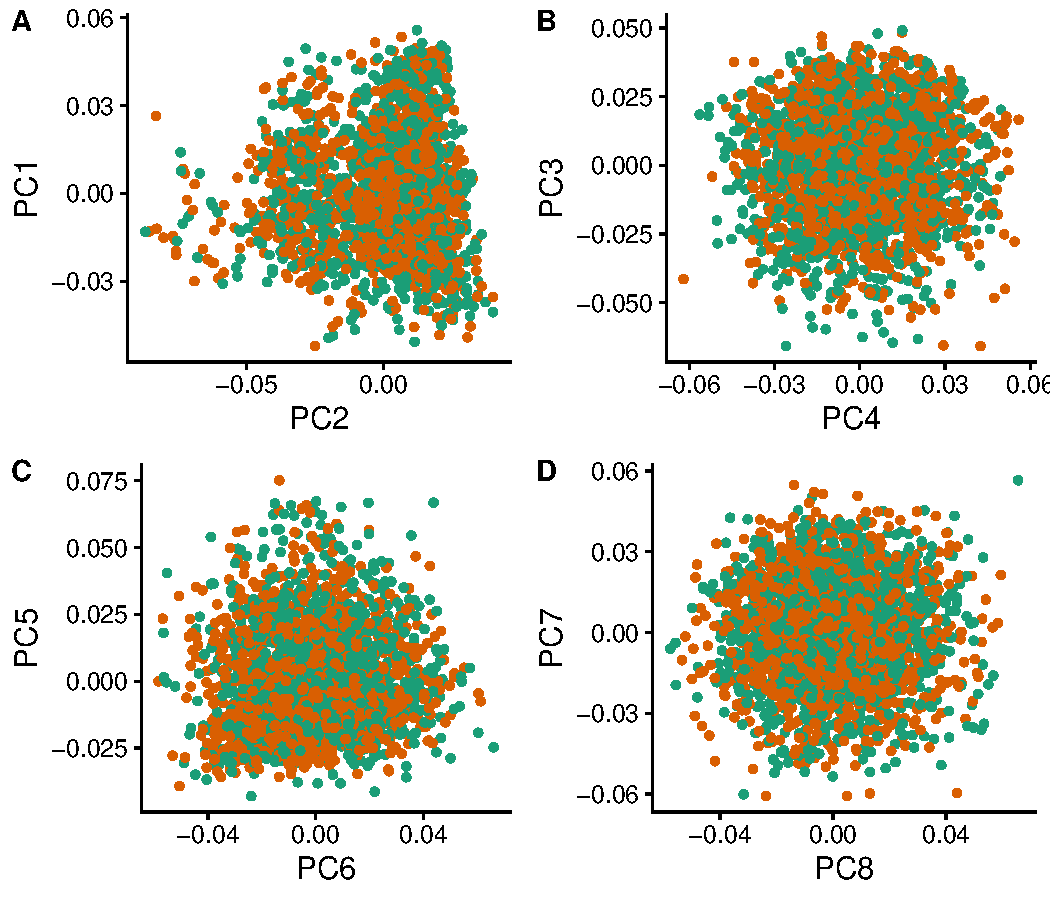
\includegraphics[width=.9\linewidth]{./figures/sfigure_1.pdf}

\paragraph*{S2 Fig.}
\label{sfig:snp_gene_manhattan}
{\bf Association in GENESIS. The red line represents the Bonferroni threshold.} \textbf{(A)}\DIFaddbegin \DIFadd{~}\DIFaddend SNP association, measured from the outcome of a 1 d.f. $\chi^2$ allelic test \DIFaddbegin \DIFadd{(Section~\ref{methods:conventional})}\DIFaddend . Significant SNPs that are within a coding gene, or within 50 kilobases of its boundaries, are annotated. The Bonferroni threshold is 2.54 \texttimes{} 10\textsuperscript{-7}. \textbf{(B)}\DIFaddbegin \DIFadd{~}\DIFaddend Gene association, measured by P\=/value of VEGAS2 \cite{mishra_vegas2:_2015} using the 10\% of SNPs with the lowest P\=/values \DIFaddbegin \DIFadd{(Section~\ref{methods:conventional})}\DIFaddend . The Bonferroni threshold is 1.53 \texttimes{} 10\textsuperscript{-6}. \textbf{(C)}\DIFaddbegin \DIFadd{~}\DIFaddend SNP association as in panel (A). The SNPs in black are selected by a L1-penalized logistic regression (Section~\ref{methods:classifier}, $\lambda = 0.03$).
%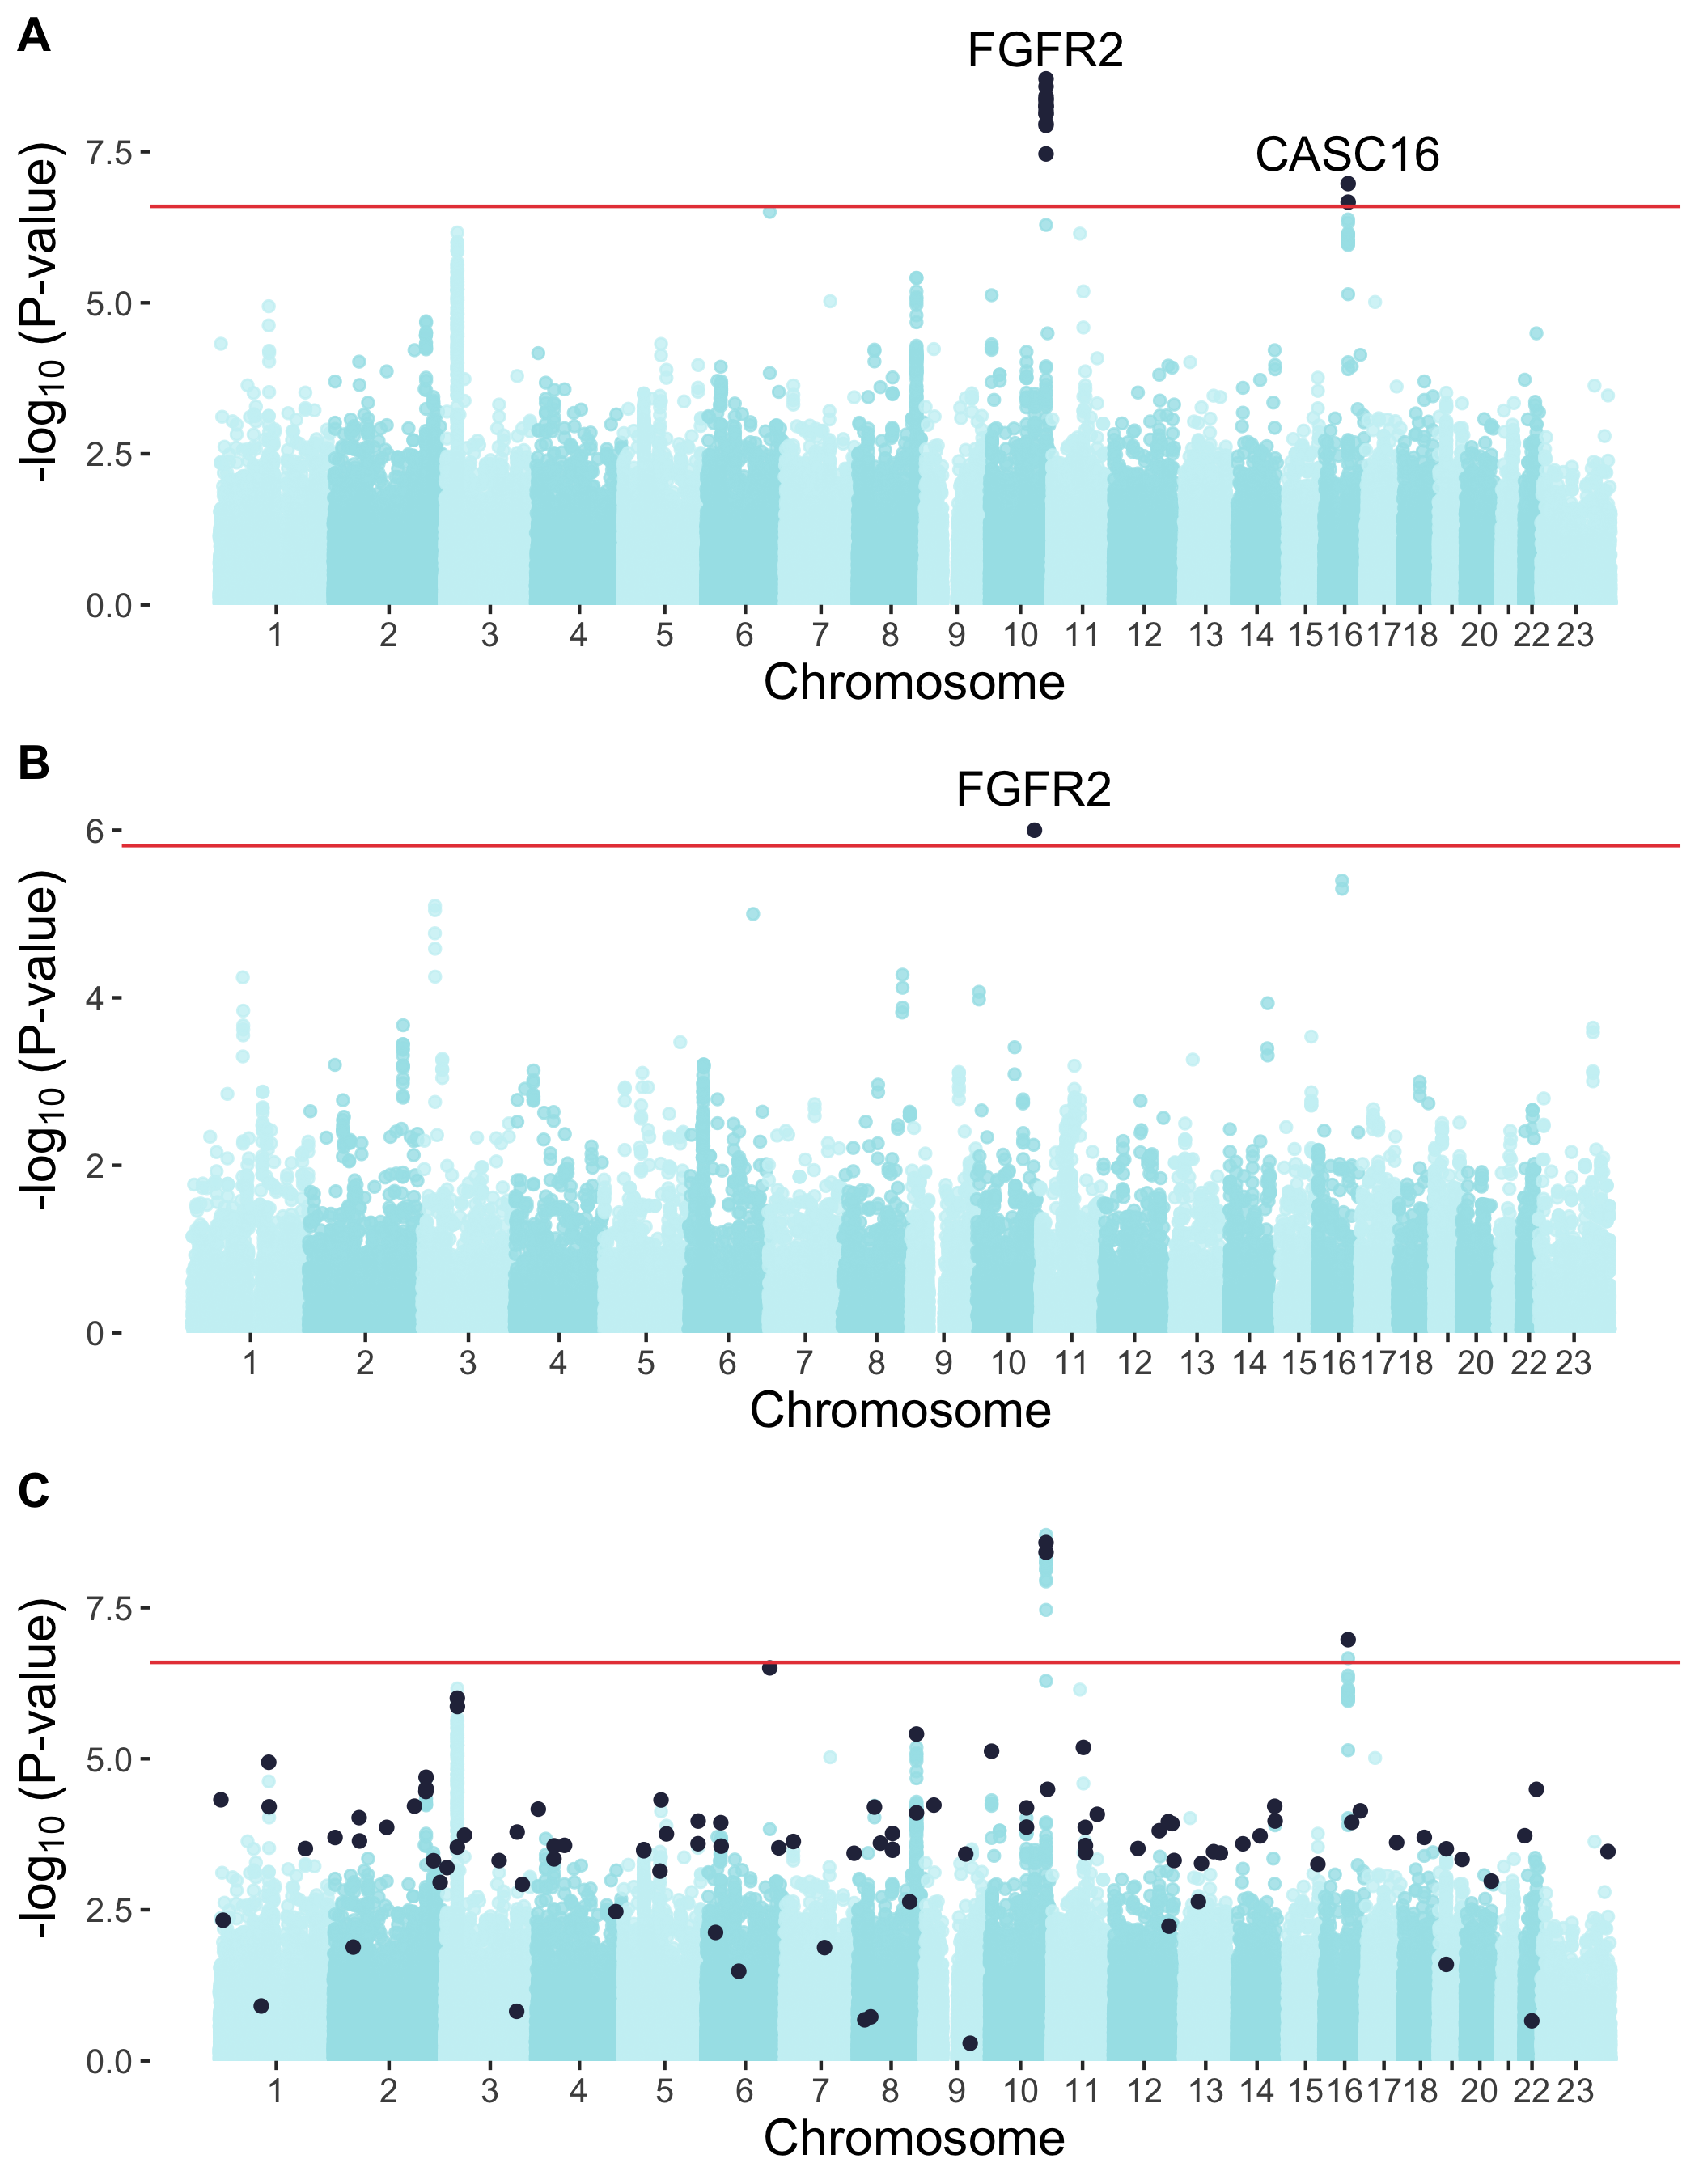
\includegraphics[width=.7\linewidth]{./figures/sfigure_2.png}

\paragraph*{S3 Fig.}
\label{sfig:pearson_methods}
{\bf Pearson correlation between the different \DIFdelbegin \DIFdel{solution subnetworks}\DIFdelend \DIFaddbegin \DIFadd{solutions}\DIFaddend . } \textbf{(A)}\DIFaddbegin \DIFadd{~}\DIFaddend Correlation between selected SNPs. \textbf{(B)}\DIFaddbegin \DIFadd{~}\DIFaddend Correlation between selected genes. In general, the solutions display a very low overlap.
%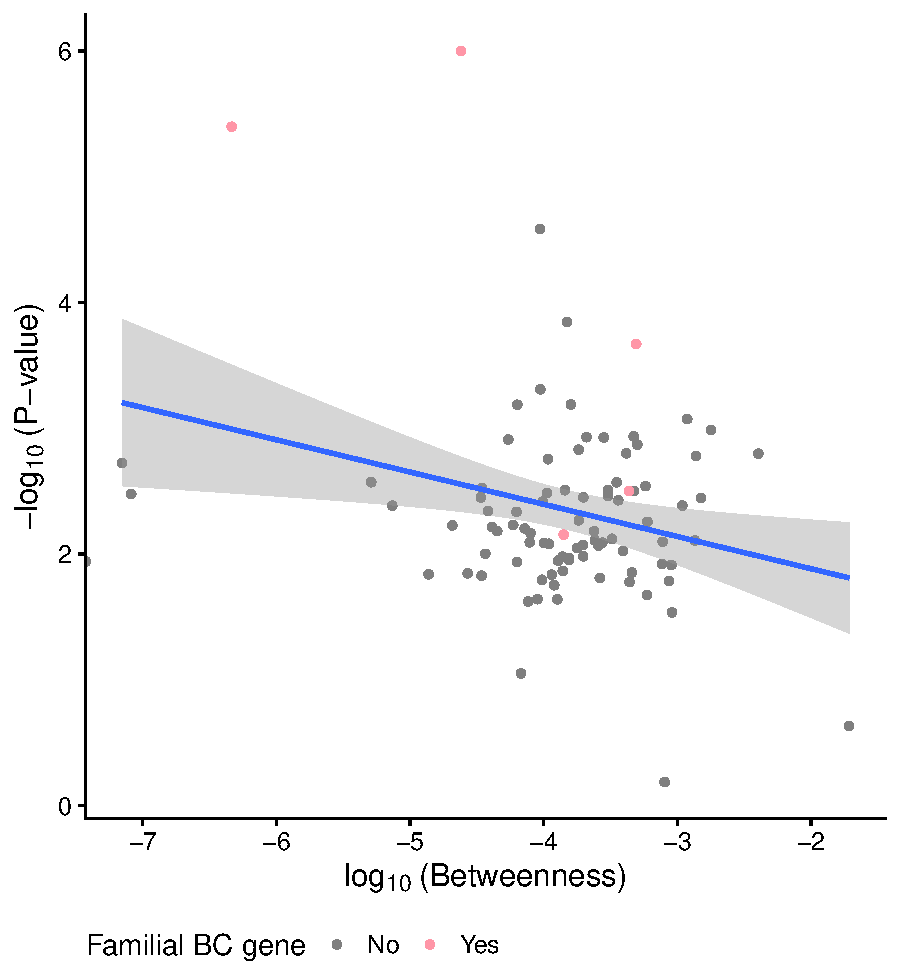
\includegraphics[width=.9\linewidth]{./figures/sfigure_3.pdf}

\paragraph*{S4 Fig.}
\label{sfig:consensus-names}
{\bf Consensus \DIFdelbegin \DIFdel{subnetwork }\DIFdelend \DIFaddbegin \DIFadd{solution }\DIFaddend on GENESIS (Section~\ref{methods:methods}). } \textbf{(A)}\DIFaddbegin \DIFadd{~}\DIFaddend Each node is represented by a pie chart, which shows the methods that selected it. We labeled (and enlarged) the two most central genes (\emph{COPS5} and \emph{OFD1}) and those genes that are known breast cancer susceptibility genes and/or significantly associated with breast cancer susceptibility in the BCAC dataset. The latter ones are also colored in pink. This panel is identical to Fig~\ref{fig:consensus}. \textbf{(B)}\DIFdelbegin \DIFdel{Same }\DIFdelend \DIFaddbegin \DIFadd{~The same }\DIFaddend network, but every gene name is indicated. \DIFaddbegin \DIFadd{We colored in pink the names of genes that are known breast cancer susceptibility genes and/or significantly associated with breast cancer susceptibility in the BCAC dataset.
}\DIFaddend % 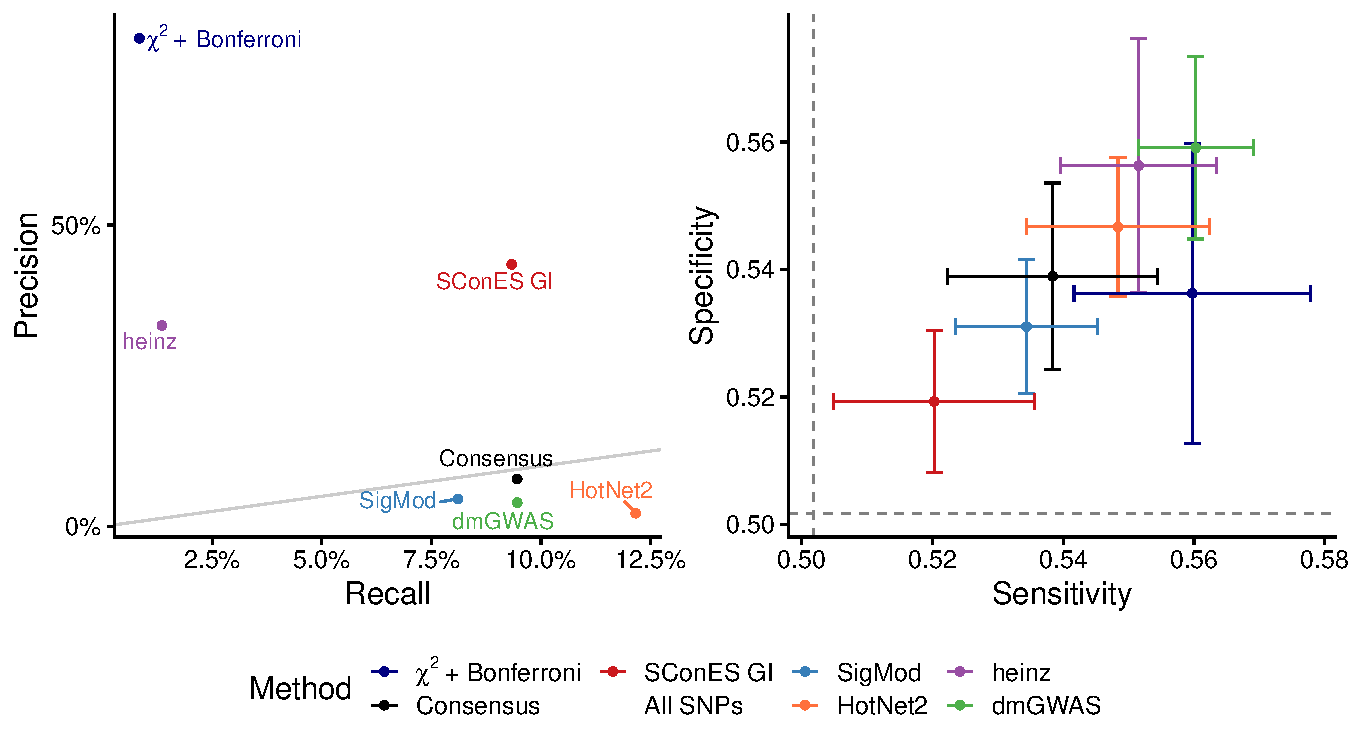
\includegraphics[width=.675\linewidth]{./figures/sfigure_4.pdf}

\paragraph*{S5 Fig.}
\label{sfig:consensus_stats}
{\bf \DIFdelbegin \DIFdel{Genes on the consensus network. Breast cancer susceptibility genes are colored in pink; the rest are colored in grey. }%DIFDELCMD < } %%%
\textbf{\DIFdel{(A)}} %DIFAUXCMD
\DIFdel{Number of methods selecting every gene in the subnetwork. }\textbf{\DIFdel{(B)}} %DIFAUXCMD
\DIFdel{VEGAS2 P\=/values of association of the genes , with regards to the number of methods that selected them. }\textbf{\DIFdel{(C)}} %DIFAUXCMD
\DIFdel{Comparison of betweenness centrality of the genes in the consensus network andthe other genes in the PPIN and not in the consensus network.
To improve visualization, we removed outliers. }\textbf{\DIFdel{(D)}} %DIFAUXCMD
\DIFdelend Relationship between the log\textsubscript{10} of the betweenness centrality and the -log\textsubscript{10} of the VEGAS2 P\=/value of the genes in the consensus \DIFdelbegin \DIFdel{network.}\DIFdelend \DIFaddbegin \DIFadd{solution.}} \DIFaddend The blue line represents a fitted generalized linear model.
% 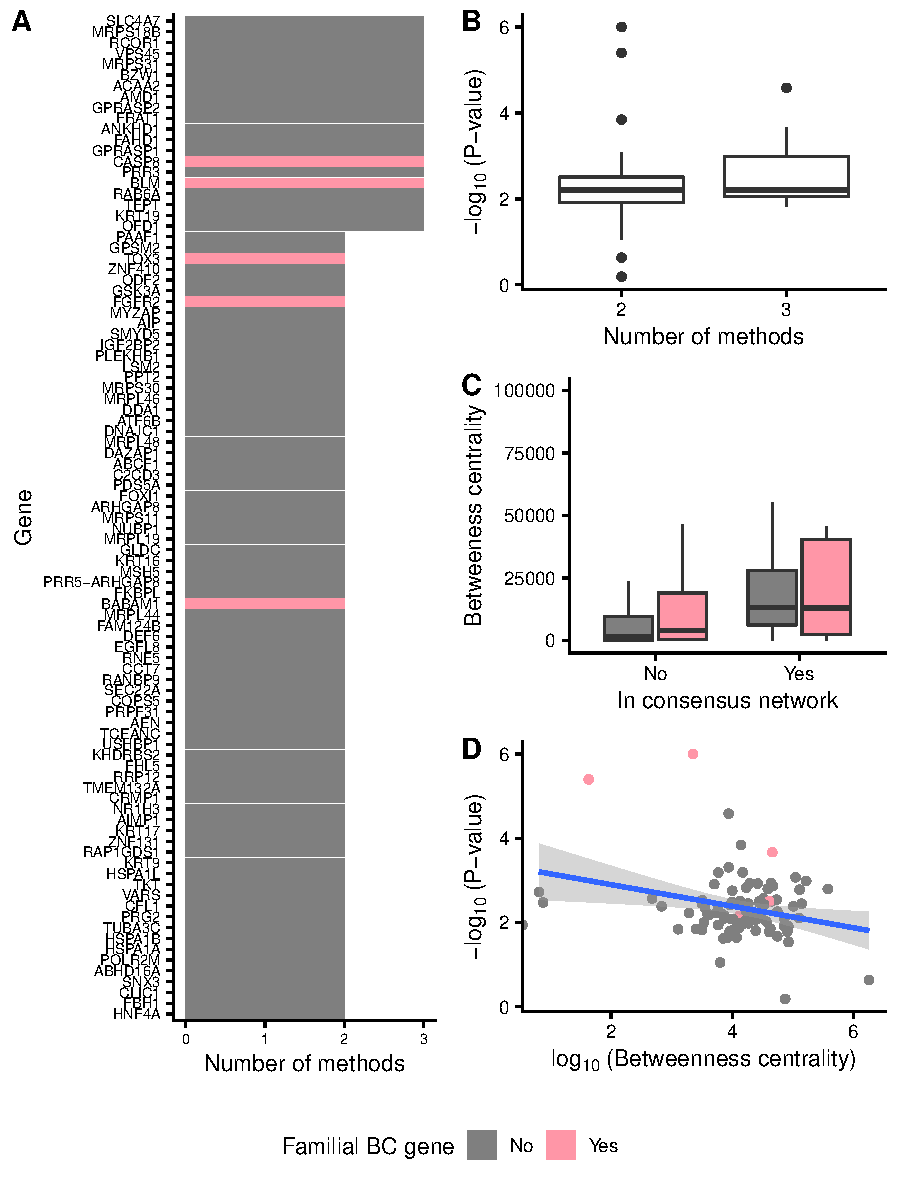
\includegraphics[width=.65\textwidth]{./figures/sfigure_5.pdf}

\paragraph*{S6 Fig.}
\DIFaddbegin \label{sfig:additional-benchmarks}
{\bf \DIFadd{Additional benchmarks of the network methods}} \textbf{\DIFadd{(A)}}\DIFadd{~Precision and recall of the evaluated methods with respect to Bonferroni-significant SNPs/genes in BCAC. For reference, we added a gray line with a slope of 1. This panel is identical to Fig~\ref{fig:consensus}. }\textbf{\DIFadd{(B)}}\DIFadd{~Sensitivity and specificity on the test set of the L1-penalized logistic regression trained on the features selected by each of the methods. The performance of the classifier trained on all SNPs is also displayed. Points are the average over the 5 runs; the error bars represent the standard error of the mean.}
%DIF >  \includegraphics[width=.675\linewidth]{./figures/sfigure_6.pdf

\paragraph*{\DIFadd{S7 Fig.}}
\DIFaddend \label{sfig:stable-consensus-names}
{\bf Stable consensus \DIFdelbegin \DIFdel{subnetwork }\DIFdelend \DIFaddbegin \DIFadd{solution }\DIFaddend on GENESIS (Section~\ref{results:stable-consensus}). } \textbf{(A)}\DIFaddbegin \DIFadd{~}\DIFaddend Each node is represented by a pie chart, which shows the methods that selected it. We labeled (and enlarged) the two most central genes (\emph{CUL3}) and those genes that are known breast cancer susceptibility genes and/or significantly associated with breast cancer susceptibility in the BCAC dataset. The latter ones are also colored in pink. This panel is identical to Fig~\ref{fig:stable-consensus}. \textbf{(B)}\DIFdelbegin \DIFdel{Same }\DIFdelend \DIFaddbegin \DIFadd{~The same }\DIFaddend network, but every gene name is indicated. %DIF <  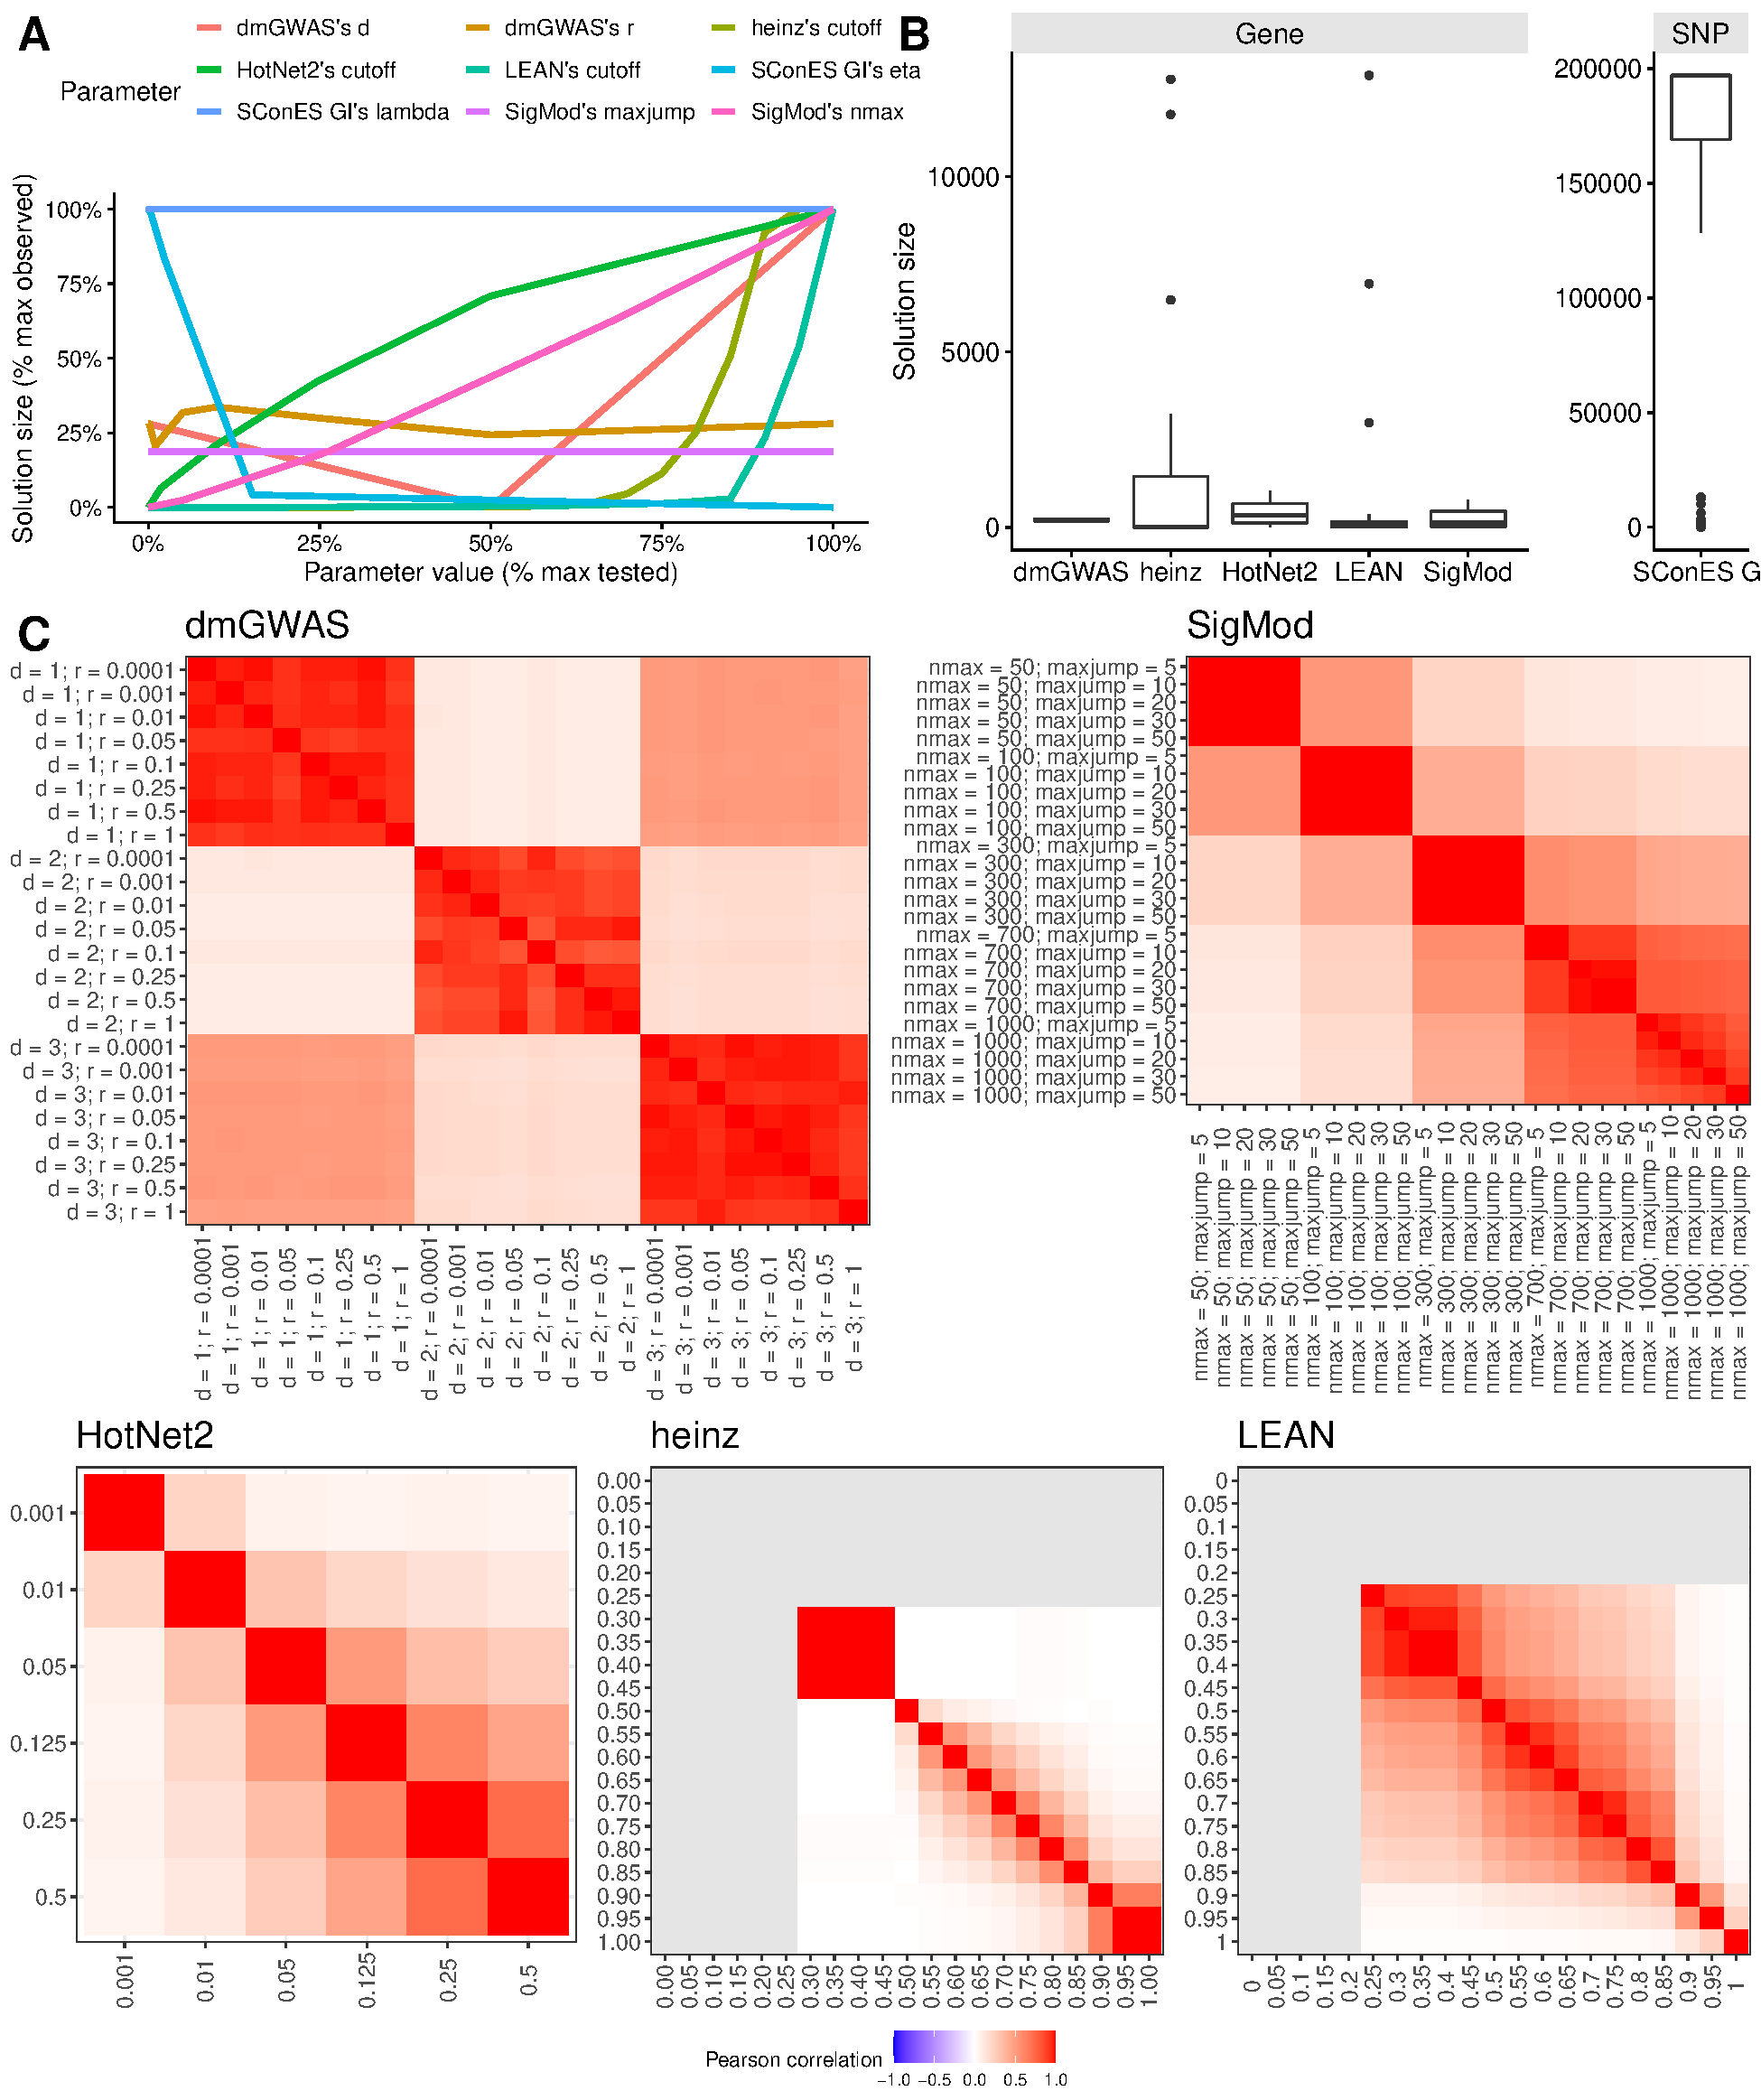
\includegraphics[width=.675\linewidth]{./figures/sfigure_6.pdf}

\DIFaddbegin \DIFadd{We colored in pink the names of genes that are known breast cancer susceptibility genes and/or significantly associated with breast cancer susceptibility in the BCAC dataset.}\DIFaddend
%DIF >  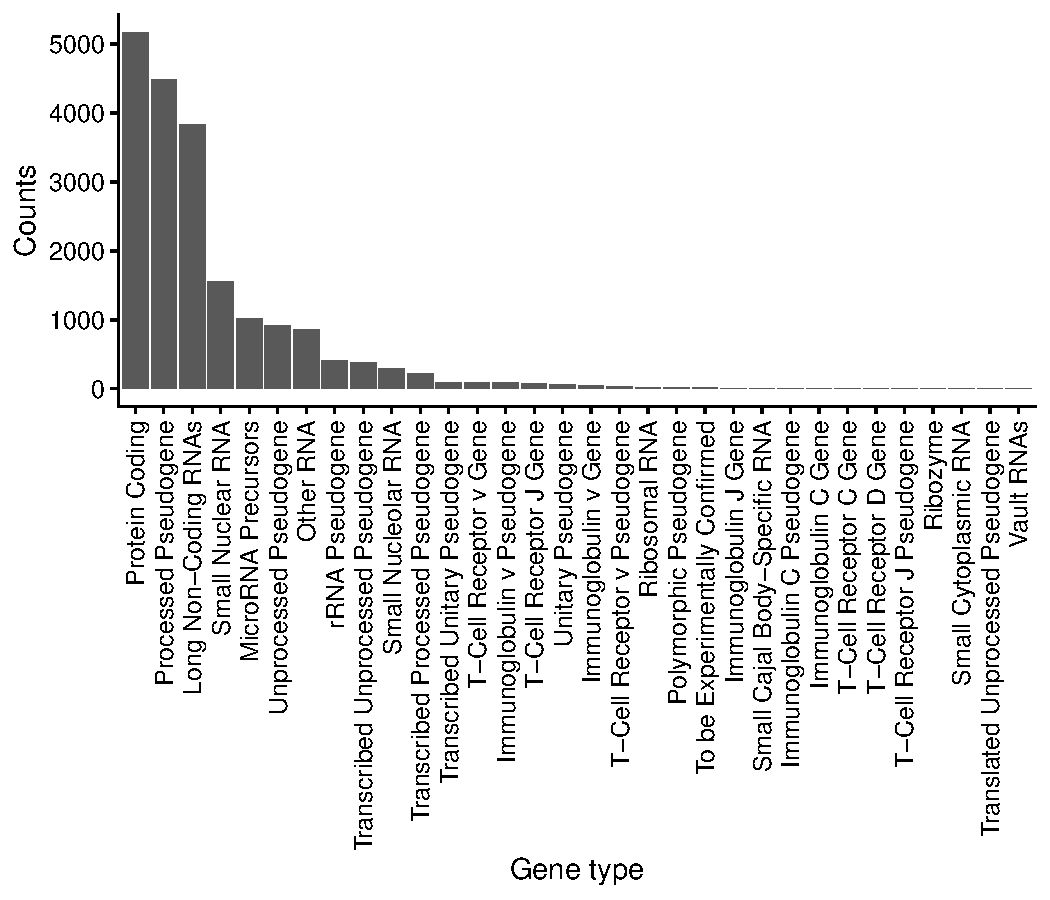
\includegraphics[width=.675\linewidth]{./figures/sfigure_7.pdf}

\paragraph*{\DIFdelbegin \DIFdel{S7 }\DIFdelend \DIFaddbegin \DIFadd{S8 }\DIFaddend Fig.}
\label{sfig:biotypes_excluded}
{\bf Biotypes of genes from the annotation that are not present in the HINT \DIFdelbegin \DIFdel{protein-protein interaction network}\DIFdelend \DIFaddbegin \DIFadd{PPIN}\DIFaddend .}
%DIF <  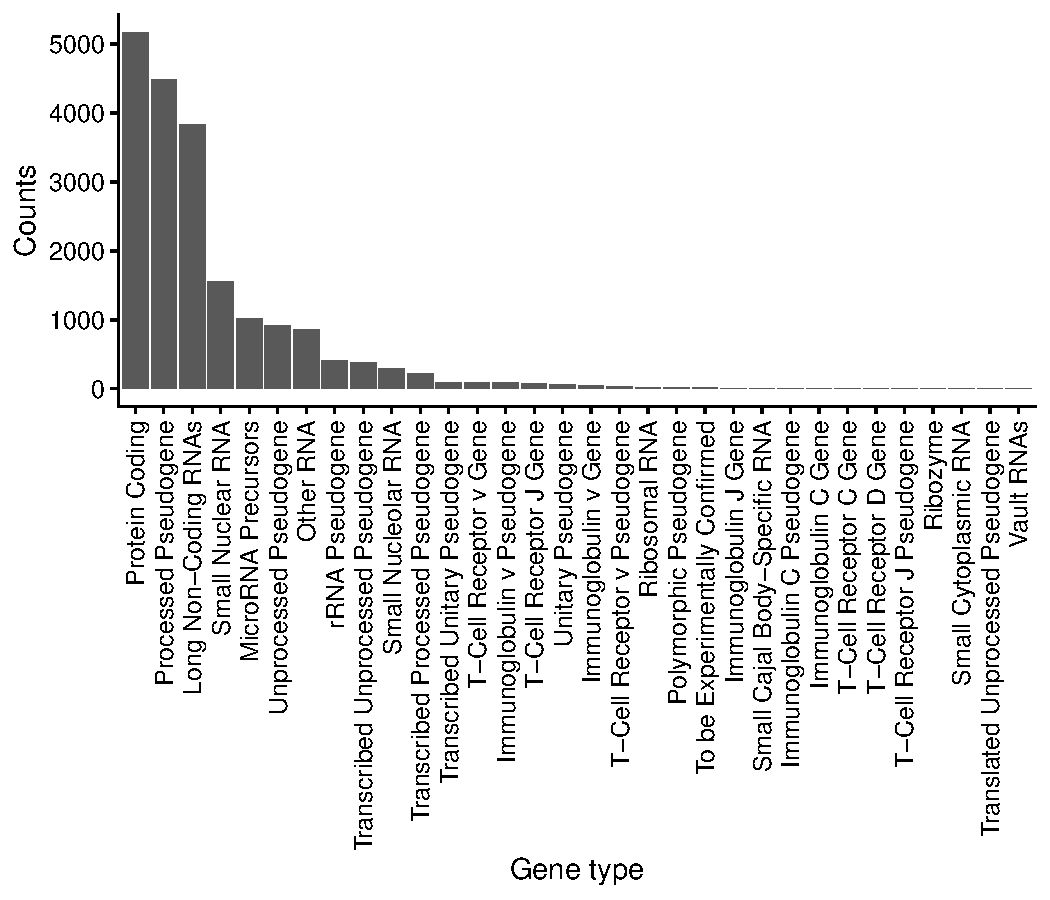
\includegraphics[width=.9\linewidth]{./figures/sfigure_7.pdf}
  
%DIF >  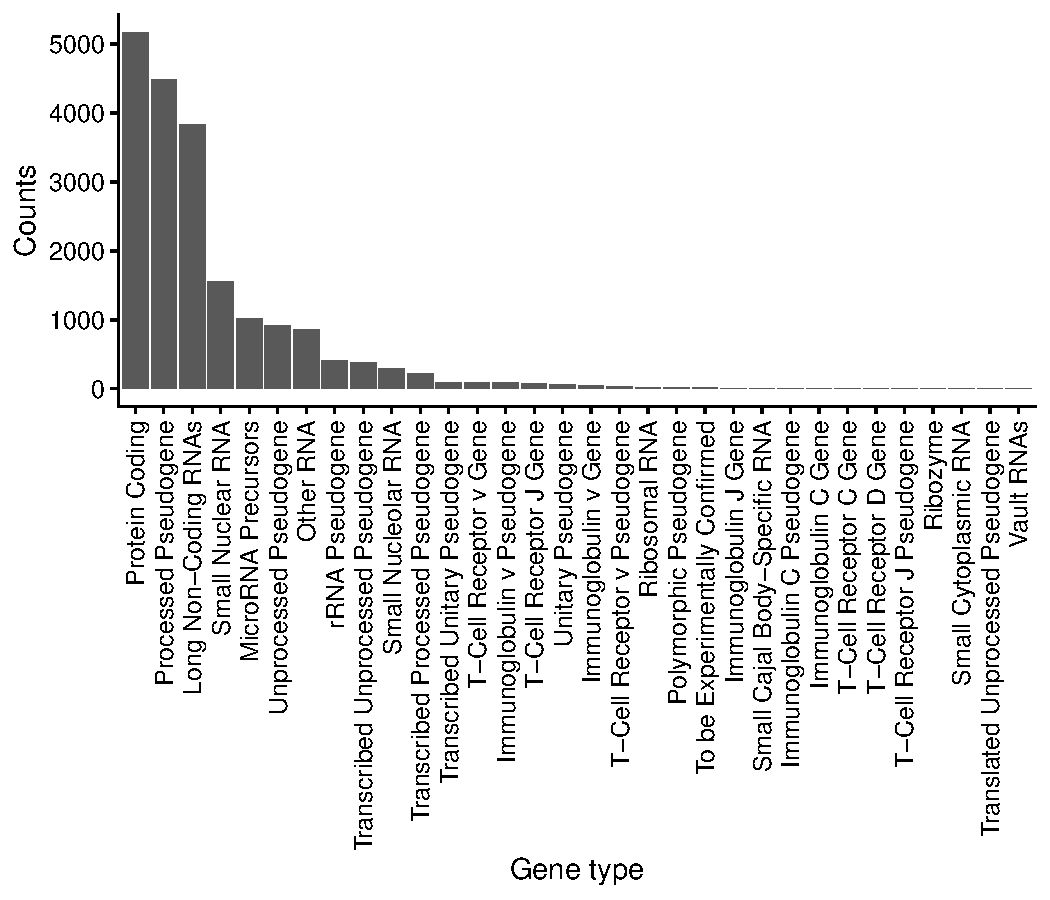
\includegraphics[width=.9\linewidth]{./figures/sfigure_8.pdf}

\paragraph*{\DIFdelbegin \DIFdel{S8 }\DIFdelend \DIFaddbegin \DIFadd{S9 }\DIFaddend Fig.}
\label{sfig:lc_ht_comparison}
{\bf Comparison of \DIFaddbegin \DIFadd{the }\DIFaddend benchmark on high-throughput (HT) interactions to \DIFaddbegin \DIFadd{the }\DIFaddend benchmark on both high-throughput and literature curated interactions (HT+LC). } Grey lines represent no change in the statistic between the benchmarks (1 for ratios mean(HT) / mean(HT + LC), 0 for differences mean(HT) - mean(HT + LC)). \textbf{(A)}\DIFaddbegin \DIFadd{~}\DIFaddend Ratios of the selected features between both benchmarks and of the active set \DIFaddbegin \DIFadd{(Section~\ref{methods:classifier})}\DIFaddend . \textbf{(B)}\DIFaddbegin \DIFadd{~}\DIFaddend Shifts in sensitivity and specificity. \textbf{(C)}\DIFaddbegin \DIFadd{~}\DIFaddend Shift in Pearson correlation between benchmarks. \textbf{(D)}\DIFaddbegin \DIFadd{~}\DIFaddend Ratio between the runtimes of the benchmarks. For \DIFdelbegin \DIFdel{gene network-based }\DIFdelend \DIFaddbegin \DIFadd{gene-based }\DIFaddend methods, inverted triangles represent the ratio of runtimes of the algorithms themselves, and circles the total time, which includes the algorithm themselves and the additional 119\,980 seconds (1 day and 9.33 hours) that VEGAS2 took on average to compute the gene scores from SNP summary statistics. In general, adding additional interactions slightly improves the stability of the solution, but increases the solution size, has mixed effects on the sensitivity and specificity, and impacts negatively the required runtime of the algorithms.
%DIF <  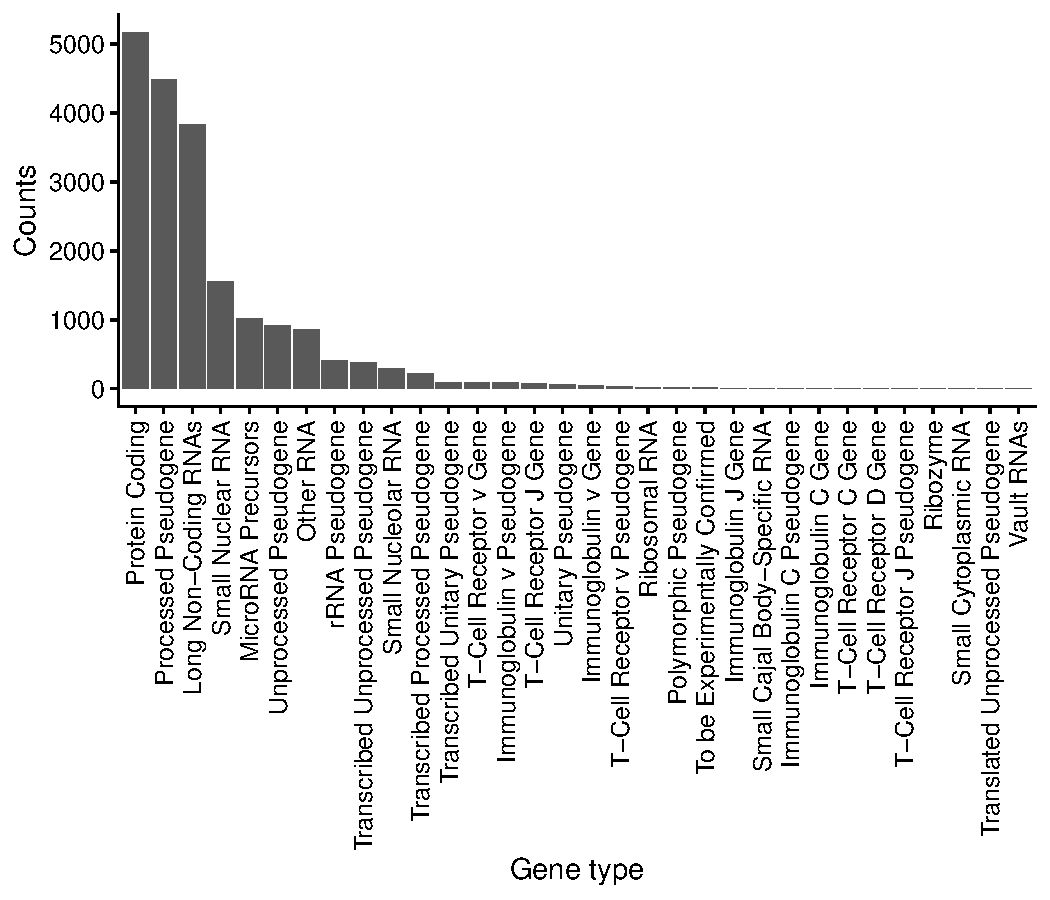
\includegraphics[width=.85\linewidth]{./figures/sfigure_8.pdf}
  
%DIF >  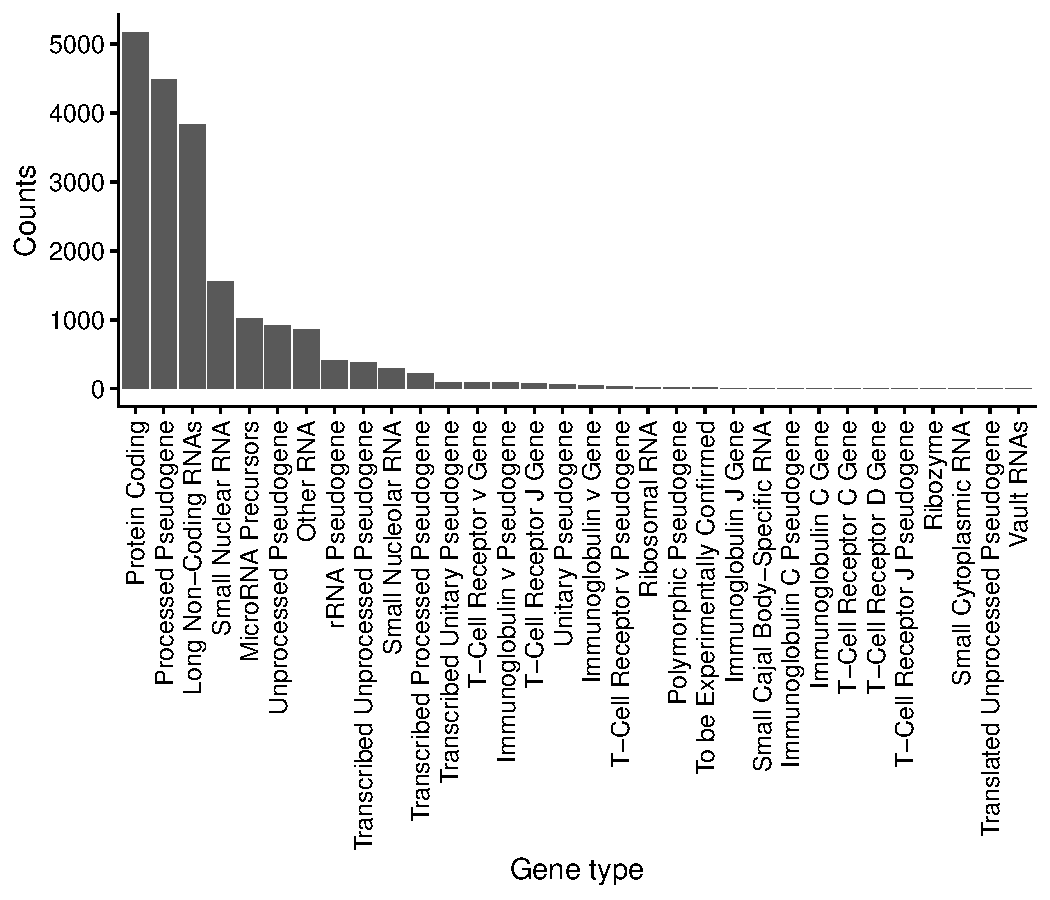
\includegraphics[width=.85\linewidth]{./figures/sfigure_9.pdf}

\paragraph*{\DIFdelbegin \DIFdel{S9 }\DIFdelend \DIFaddbegin \DIFadd{S10 }\DIFaddend Fig.}
\label{sfig:scones_gsm}
{\bf Overview of the solutions produced by the SConES on the GS and GM networks (Section \ref{methods:networks}) on the GENESIS dataset.} \textbf{(A)}\DIFaddbegin \DIFadd{~}\DIFaddend Manhattan plots of SNPs \DIFaddbegin \DIFadd{(Section \ref{methods:conventional})}\DIFaddend ; in black, the method’s solution. The Bonferroni threshold (2.54 \texttimes{} 10\textsuperscript{-7}) is indicated by a red line. \textbf{(B)}\DIFaddbegin \DIFadd{~}\DIFaddend Precision and recall of the evaluated methods with respect to Bonferroni-significant SNPs (SConES) or genes (other methods) in BCAC. For reference, we added a gray line with a slope of 1. \textbf{(C)}\DIFaddbegin \DIFadd{~}\DIFaddend Solution networks.
%DIF <  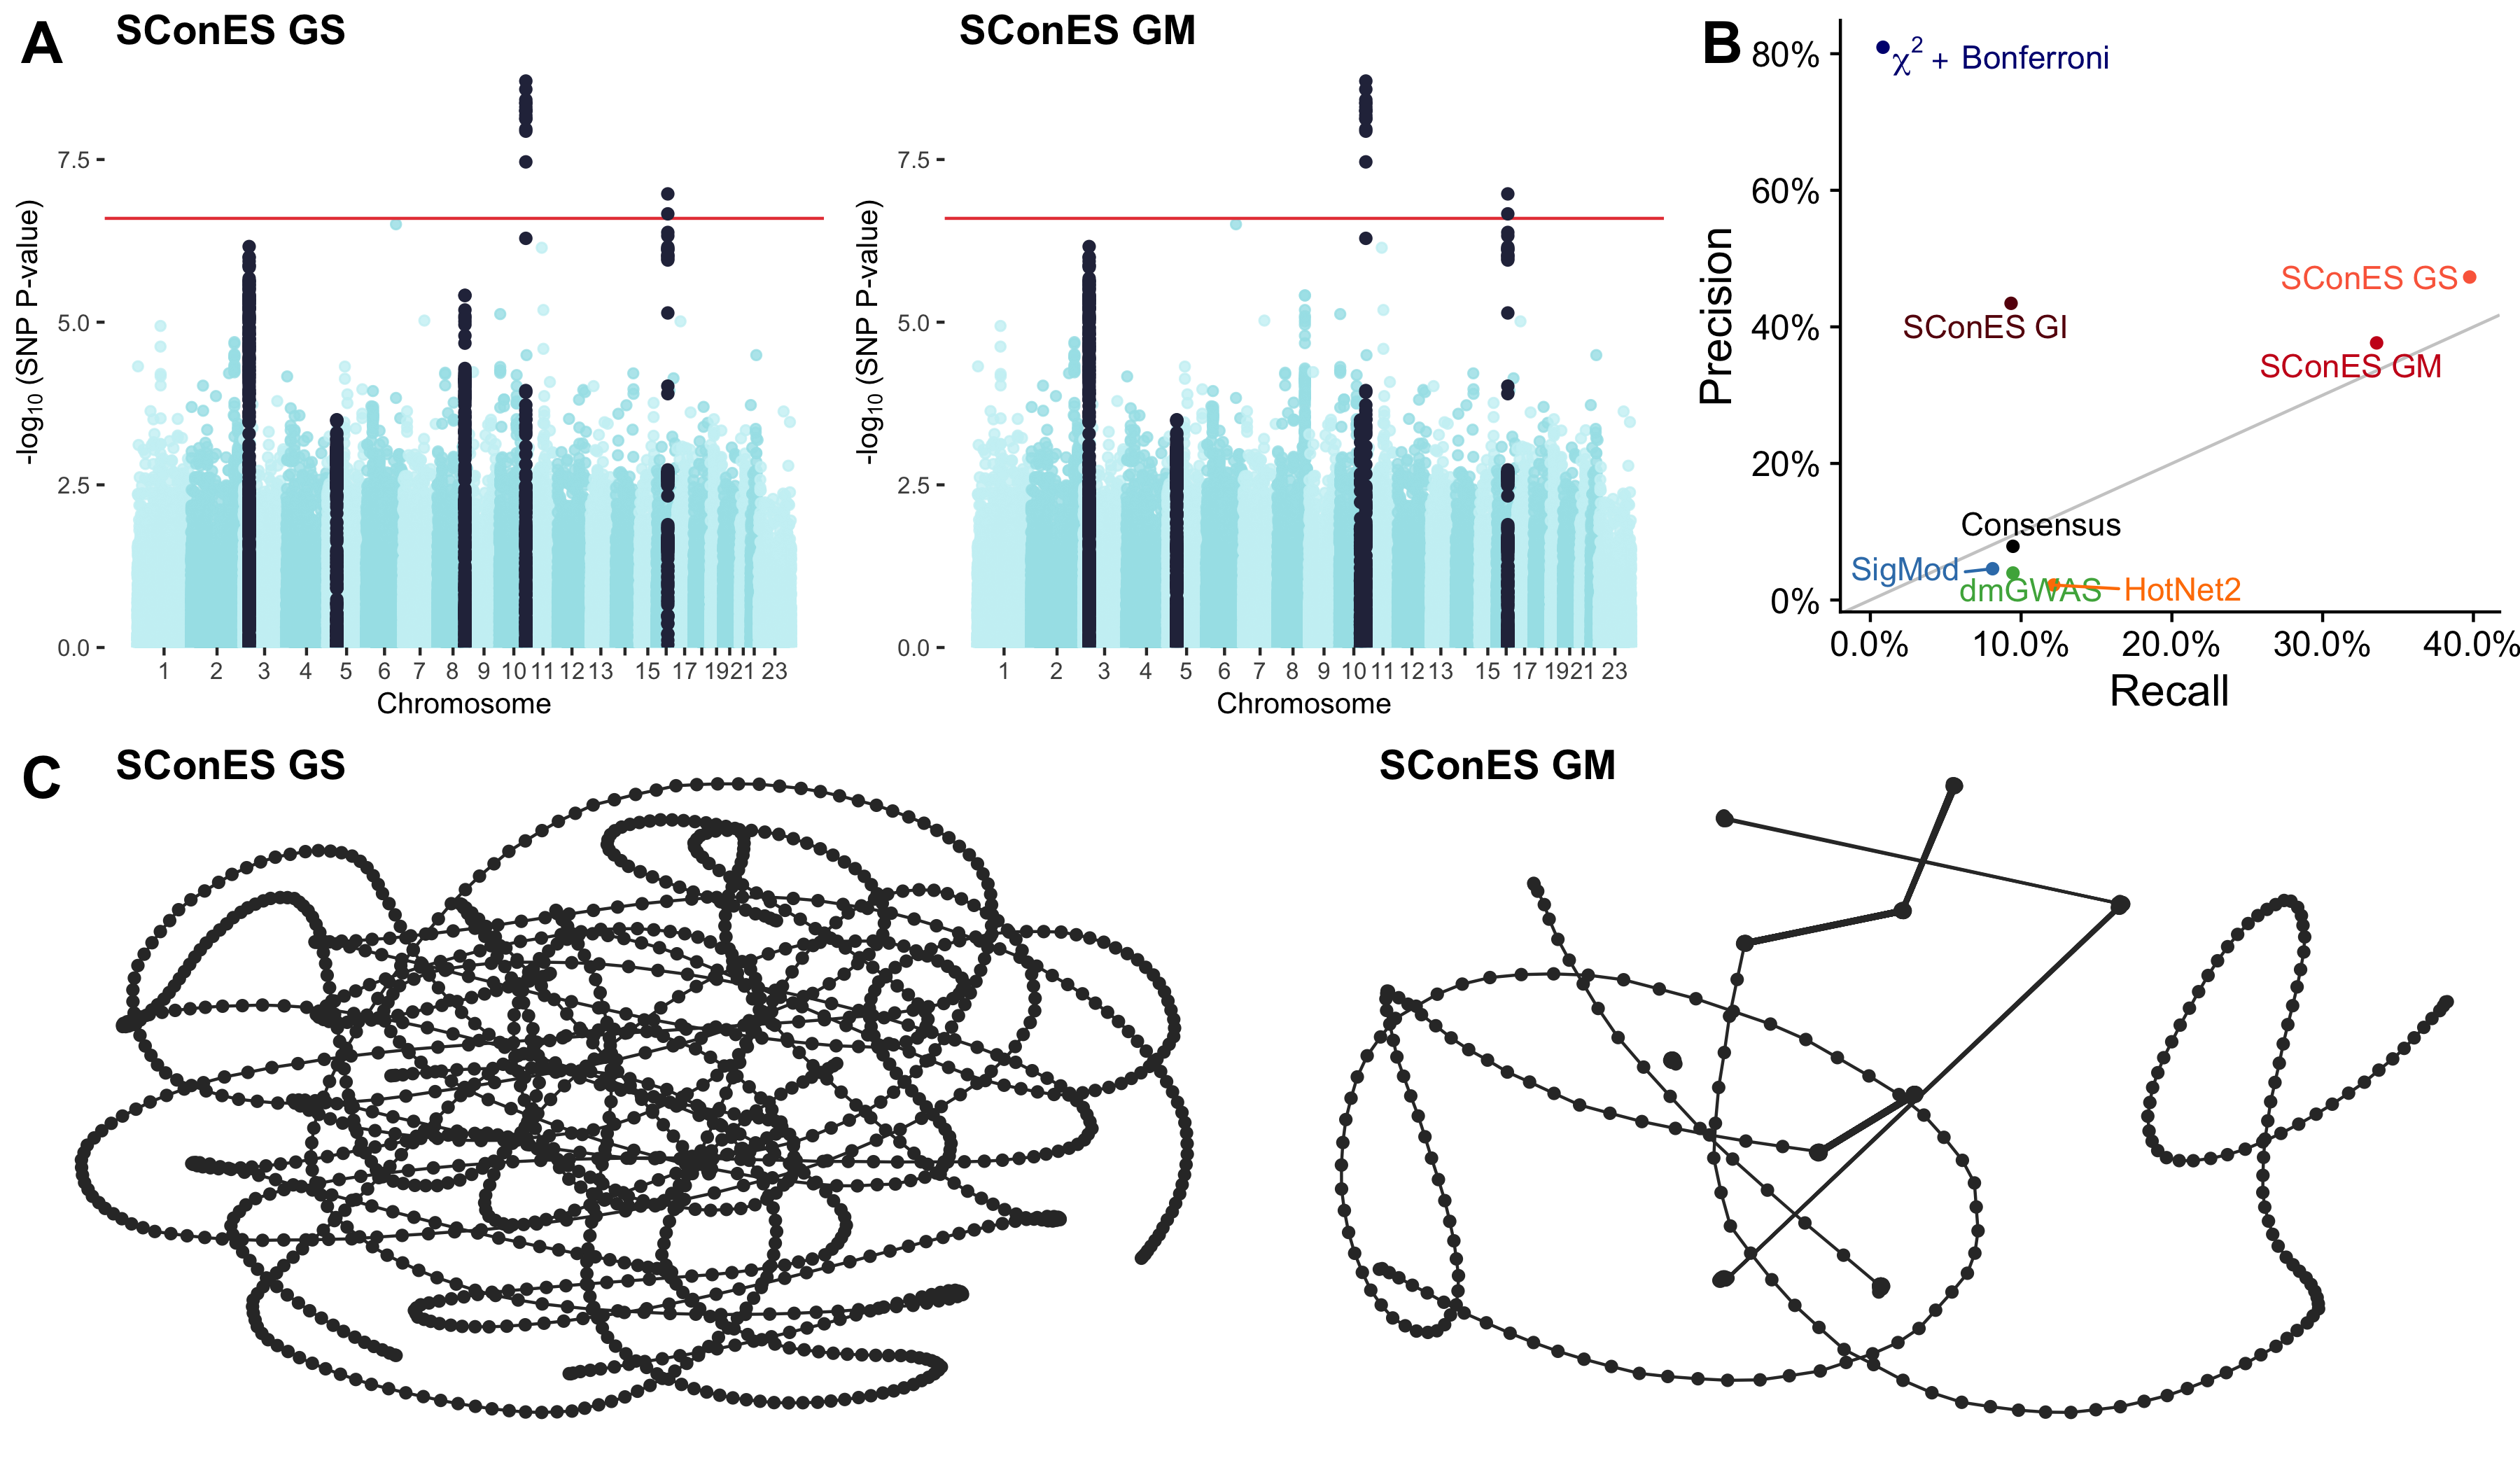
\includegraphics[width=\linewidth]{./figures/sfigure_9.png}

%DIF >  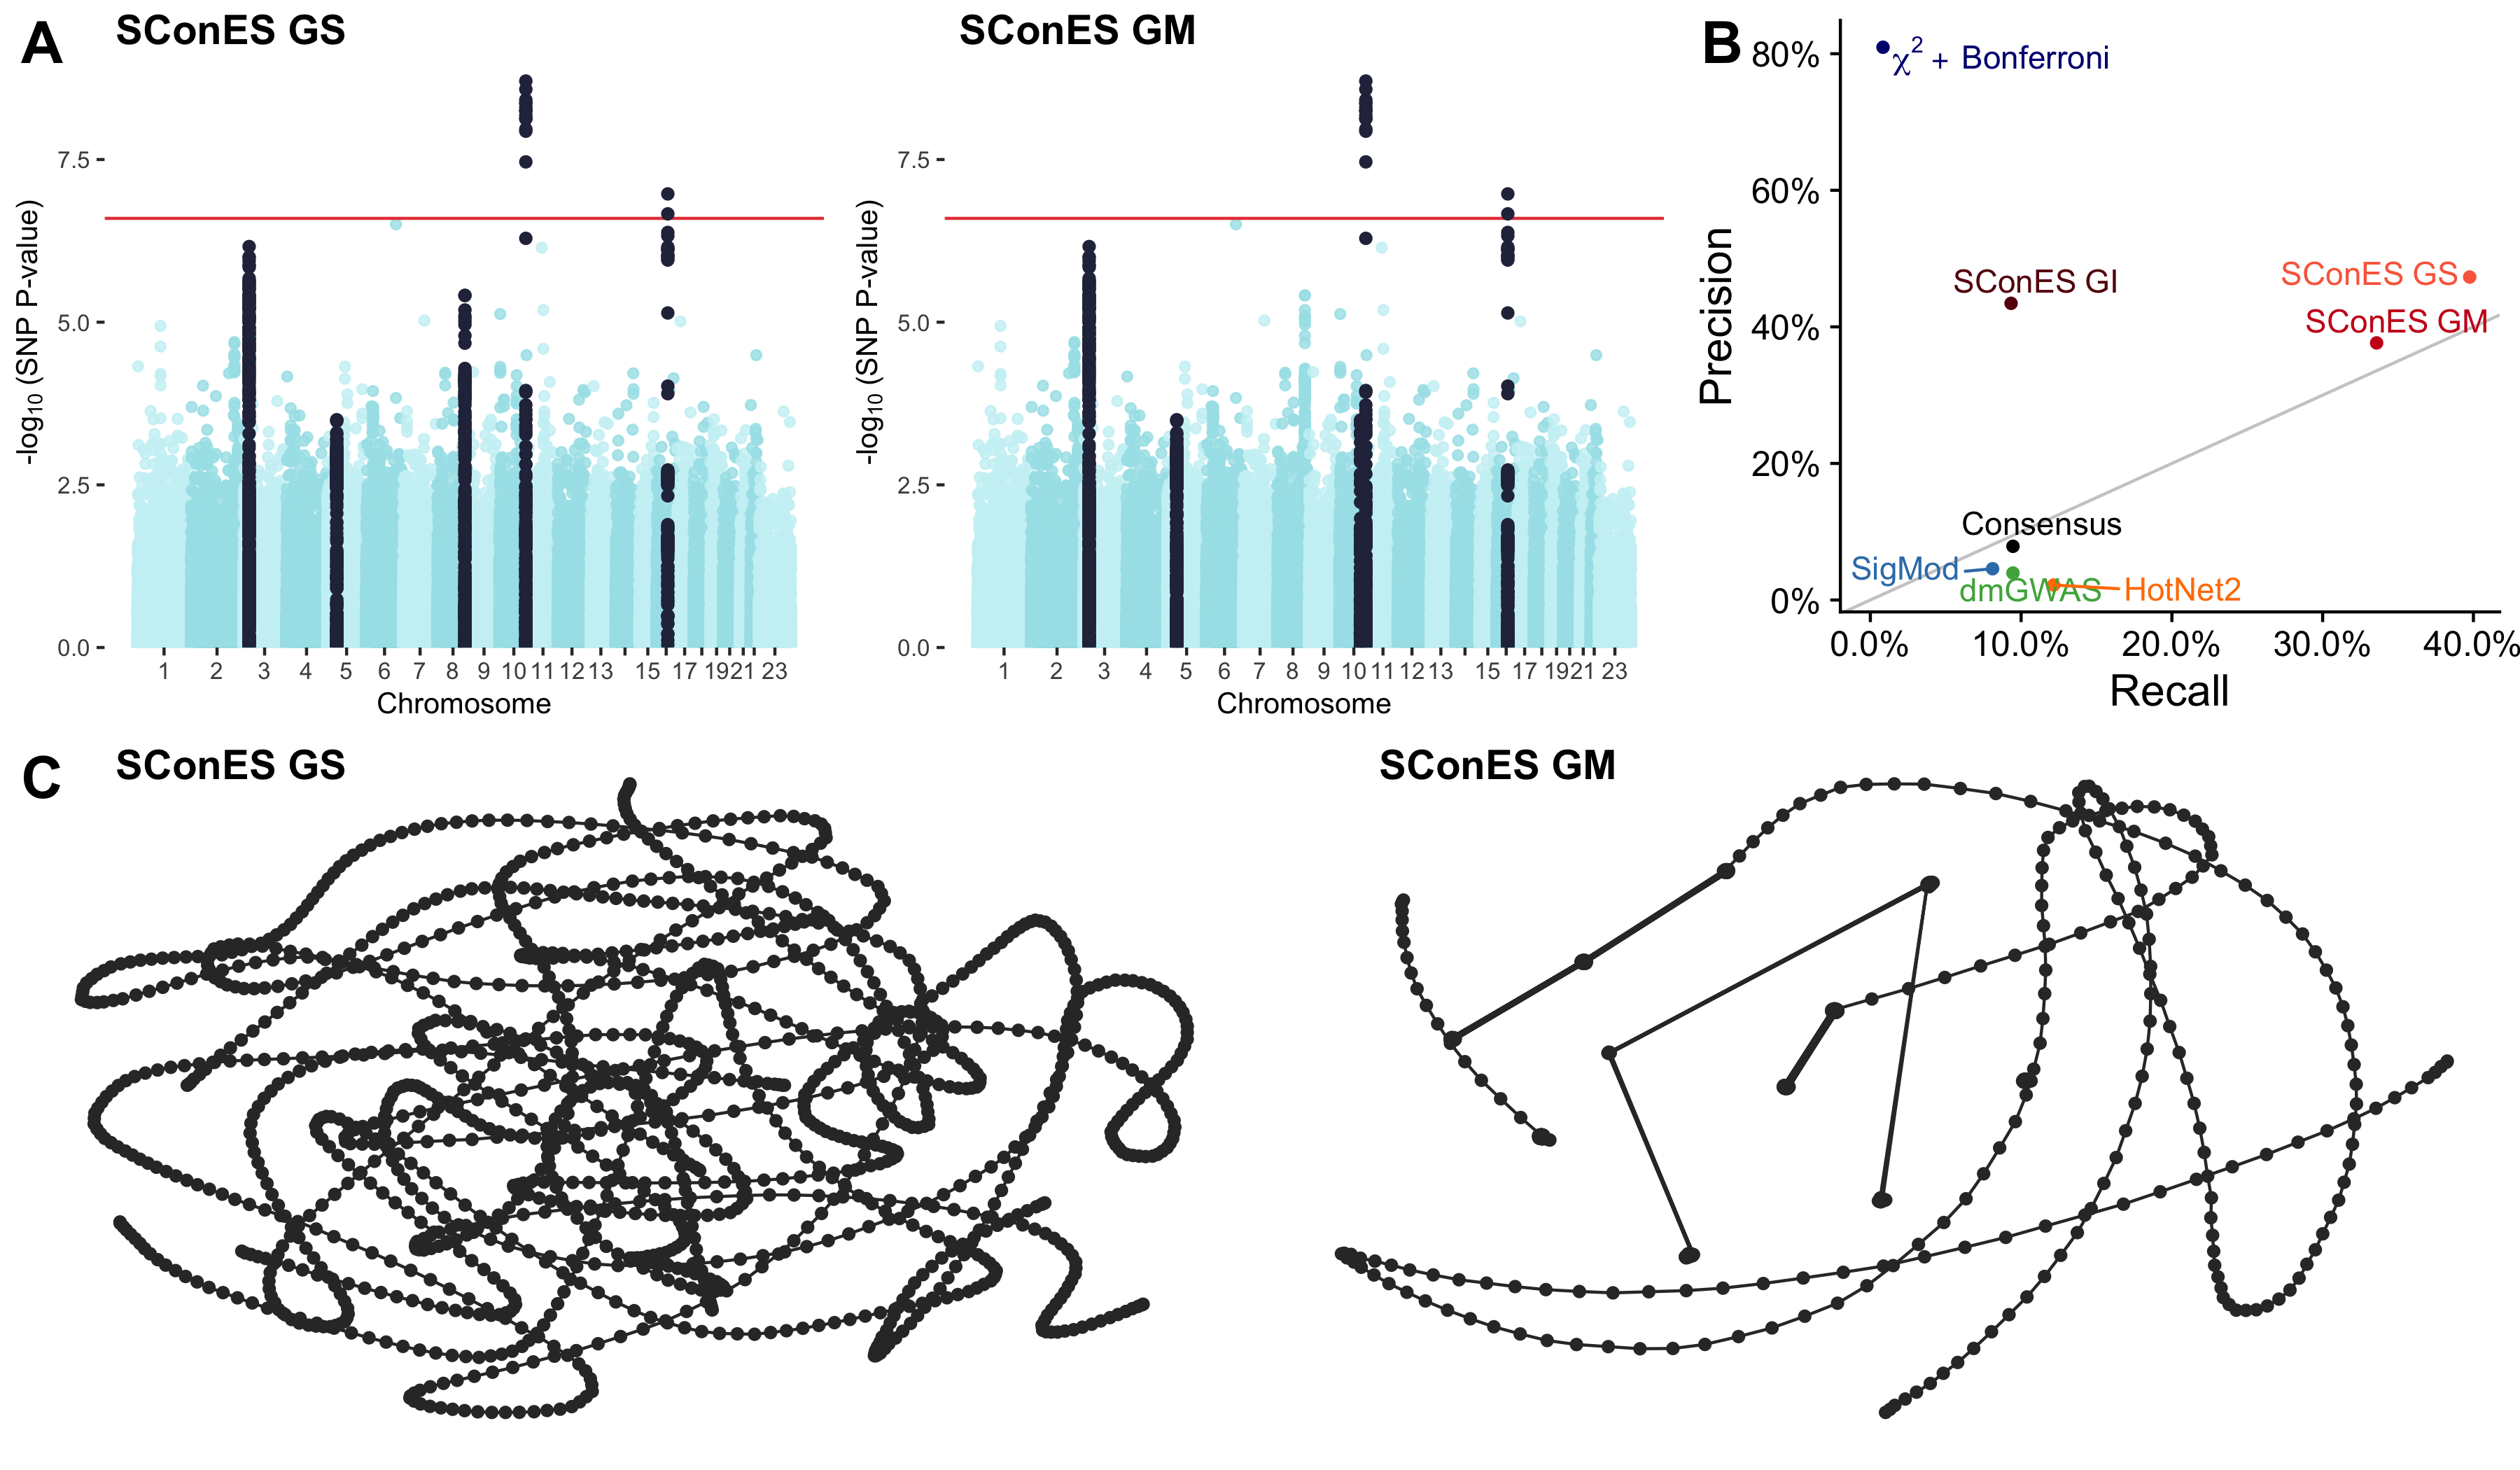
\includegraphics[width=\linewidth]{./figures/sfigure_10.png}

\section*{Acknowledgments}

\DIFaddbegin 

\DIFaddend We wish to thank Om Kulkarni for helpful discussion on gene-based GWAS and PPIN databases, and the genetic epidemiology platform (the PIGE, Plateforme d'Investigation en Génétique et Epidemiologie\DIFaddbegin \DIFadd{: S. Eon-Marchais, M. Marcou, D. Le Gal, L. Toulemonde, J. Beauvallet, N. Mebirouk, E. Cavaciuti}\DIFaddend ), the biological resource centre \DIFdelbegin \DIFdel{and }\DIFdelend \DIFaddbegin \DIFadd{(S. Mazoyer, F. Damiola, L. Barjhoux, C. Verny-Pierre, V. Sornin). We wish to pay a tribute to Olga M. Sinilnikova, who was one of the initiators and principal investigators of GENESIS and who died prematurely on June 30, 2014.}

\DIFadd{We thank }\DIFaddend all the GENESIS collaborating cancer clinics clinics \DIFaddbegin \DIFadd{(Clinique Sainte Catherine, Avignon: H. Dreyfus; Hôpital Saint Jacques, Besançon: M-A}\DIFaddend . \DIFaddbegin \DIFadd{Collonge-Rame; Institut Bergonié, Bordeaux: M.Longy, A. Floquet, E. Barouk-Simonet; CHU, Brest: S. Audebert; Centre François Baclesse, Caen: P. Berthet; Hôpital Dieu, Chambéry: S. Fert-Ferrer; Centre Jean Perrin, Clermont-Ferrand: Y-J. Bignon; Hôpital Pasteur, Colmar: J-M. Limacher; Hôpital d’Enfants CHU – Centre Georges François Leclerc, Dijon: L. Faivre-Olivier; CHU, Fort de France: O. Bera; CHU Albert Michallon, Grenoble: D. Leroux; Hôpital Flaubert, Le Havre: V. Layet; Centre Oscar Lambret, Lille: P. Vennin, C. Adenis; Hôpital Jeanne de Flandre, Lille: S. Lejeune-Dumoulin, S. Manouvier-Hanu; CHRU Dupuytren, Limoges: L. Venat-Bouvet; Centre Léon Bérard, Lyon: C. Lasset, V. Bonadona; Hôpital Edouard Herriot, Lyon: S. Giraud; Institut Paoli-Calmettes, Marseille: F. Eisinger, L. Huiart; Centre Val d’Aurelle – Paul Lamarque, Montpellier: I. Coupier; CHU Arnaud de Villeneuve, Montpellier: I. Coupier, P. Pujol; Centre René Gauducheau, Nantes: C. Delnatte; Centre Catherine de Sienne, Nantes: A. Lortholary; Centre Antoine Lacassagne, Nice: M. Frénay, V. Mari; Hôpital Caremeau, Nîmes: J. Chiesa; Réseau Oncogénétique Poitou Charente, Niort: P. Gesta; Institut Curie, Paris: D. Stoppa-Lyonnet, M. Gauthier-Villars, B. Buecher, A. de Pauw, C. Abadie, M. Belotti; Hôpital Saint-Louis, Paris: O. Cohen-Haguenauer; Centre Viggo-Petersen, Paris: F. Cornélis; Hôpital Tenon, Paris: A. Fajac; GH Pitié Salpétrière et Hôpital Beaujon, Paris: C. Colas, F. Soubrier, P. Hammel, A. Fajac; Institut Jean Godinot, Reims: C. Penet, T. D. Nguyen; Polyclinique Courlancy, Reims: L. Demange*, C. Penet; Centre Eugène Marquis, Rennes: C. Dugast*; Centre Henri Becquerel, Rouen: A. Chevrier, T. Frebourg, J. Tinat, I. Tennevet, A. Rossi; Hôpital René Huguenin/Institut Curie, Saint Cloud: C. Noguès, L. Demange*, E. Mouret-Fourme; CHU, Saint-Etienne: F. Prieur; Centre Paul Strauss, Strasbourg: J-P. Fricker, H. Schuster; Hôpital Civil, Strasbourg: O. Caron, C. Maugard; Institut Claudius Regaud, Toulouse: L. Gladieff, V. Feillel; Hôpital Bretonneau, Tours: I. Mortemousque; Centre Alexis Vautrin, Vandoeuvre-les-Nancy: E. Luporsi; Hôpital de Bravois, Vandoeuvre-les-Nancy: P. Jonveaux; Gustave Roussy, Villejuif: A. Chompret*, O. Caron).
*Deceased prematurely}\DIFaddend 

\section*{Author contributions}

\begin{description}
  \item[Conceptualization] Héctor Climente-González, Christine Lonjou, Chloé-Agathe Azencott.
  \item[Data curation] Christine Lonjou, GENESIS Study collaborators.
  \item[Formal Analysis] Héctor Climente-González, Christine Lonjou.
  \item[Funding acquisition] Dominique Stoppa-Lyonnet, Nadine Andrieu, Chloé-Agathe Azencott.
  \item[Investigation] Héctor Climente-González, Christine Lonjou.
  \item[Methodology] Héctor Climente-González, Christine Lonjou, Chloé-Agathe Azencott.
  \item[Project administration] Chloé-Agathe Azencott.
  \item[Resources] GENESIS Study collaborators, Dominique Stoppa-Lyonnet, Nadine Andrieu.
  \item[Software] Héctor Climente-González, Christine Lonjou.
  \item[Supervision] Christine Lonjou, Fabienne Lesueur, Nadine Andrieu, Chloé-Agathe Azencott.
  \item[Validation] Christine Lonjou, Fabienne Lesueur.
  \item[Visualization] Héctor Climente-González.
  \item[Writing – original draft] Héctor Climente-González.
  \item[Writing – review \& editing] Héctor Climente-González, Christine Lonjou, Fabienne Lesueur, Nadine Andrieu, Chloé-Agathe Azencott.
\end{description}

\nolinenumbers

\bibliography{bibliography.bib}

% Either type in your references using
% \begin{thebibliography}{}
% \bibitem{}
% Text
% \end{thebibliography}
%
% or
%
% Compile your BiBTeX database using our plos2015.bst
% style file and paste the contents of your .bbl file
% here. See http://journals.plos.org/plosone/s/latex for 
% step-by-step instructions.
% 

\end{document}
